% !TeX program = lualatex
% MAKE53の全訳。数式・数値・引用・図表番号は英語版に対応する。
% 再コンパイル：lualatex main_paper_NN53.tex（参照確定まで2回）
\documentclass[11pt,a4paper]{ltjsarticle}
\usepackage[haranoaji]{luatexja-preset}
\usepackage{fix-cm}
\usepackage{amsmath,amsthm,amssymb,mathtools}
\usepackage{graphicx,booktabs,array,multirow,tabularx,here}
\usepackage{enumitem}
\usepackage[margin=23mm]{geometry}
\usepackage[numbers,sort&compress]{natbib}
\usepackage{xurl}
\usepackage[unicode,hidelinks]{hyperref}
\usepackage{caption}
\usepackage{etoolbox}
\setmainfont{TeX Gyre Pagella}
\setsansfont{TeX Gyre Heros}
\setmonofont{Latin Modern Mono}[Scale=MatchLowercase]
\captionsetup{font=small,labelfont=bf}
\setlist[enumerate]{leftmargin=2em,itemsep=2pt,topsep=4pt}
\emergencystretch=2em
\setlength{\tabcolsep}{3.5pt}
\renewcommand{\arraystretch}{1.12}
\newtheorem{Algorithm}{アルゴリズム}
\appto{\appendix}{%
 \renewcommand{\thesection}{\Alph{section}}%
 \setcounter{table}{0}\renewcommand{\thetable}{A\arabic{table}}%
 \renewcommand{\theHtable}{A\arabic{table}}%
 \setcounter{figure}{0}\renewcommand{\thefigure}{A\arabic{figure}}%
 \renewcommand{\theHfigure}{A\arabic{figure}}%
 \setcounter{equation}{0}\renewcommand{\theequation}{A\arabic{equation}}%
 \renewcommand{\theHequation}{A\arabic{equation}}%
 \setcounter{Algorithm}{0}\renewcommand{\theAlgorithm}{A\arabic{Algorithm}}%
 \renewcommand{\theHAlgorithm}{A\arabic{Algorithm}}}
\renewcommand{\refname}{参考文献}
\AtBeginEnvironment{thebibliography}{\interlinepenalty=10000}
\hypersetup{pdftitle={変分自己符号化器の内在次元誘導によるボトルネック選択と活性ユニット診断},
 pdfauthor={小端 千佳，代 美月，神野 健哉},pdflang={ja-JP}}
\title{変分自己符号化器の内在次元誘導による\\ボトルネック選択と活性ユニット診断}
\author{小端 千佳，代 美月，神野 健哉\\
東京都市大学 情報工学部 知能情報工学科\\
{\small 〒158-8557 東京都世田谷区玉堤1-28-1}\\
{\small g2332016@tcu.ac.jp（C.O.），g2591402@tcu.ac.jp（M.D.）}\\
{\small 連絡著者：kjinno@tcu.ac.jp，電話：+81-3-5707-0104（K.J.）}}
\date{}
\begin{document}
\maketitle
\begin{abstract}
内在次元推定と活性ユニット診断は，変分自己符号化器のボトルネック選択の異なる側面を扱う。
4種類の画像データセット，5学習シード，5正則化重みについて，検証品質目標と共通の保存候補費用を用いて探索方策を評価する。
開始次元数のアブレーションでは，信頼性判定，fallback，参照群の費用計上を固定する。
IDが採用されるのはMNISTの25条件だけである。ID由来の開始点と判定付き中点は同じ次元数を選び，
平均要求候補数はそれぞれ8.84件，5.84件である。残る75条件は同じ昇順fallbackを用いる。
100種類の係数・閾値組合せと100種類のデータセット・重み・シード条件からなる10,000件のreplay評価で，
局所探索の155出力が品質を満たす最小次元を逃す。
各データセット3シードの剪定実験では，選択されたnativeモデルの再構成と，通常の変分自己符号化器への次元転用を区別する。
ローカルな関連度事前分布の変種では，非選択軸のマスクによりdSpritesの検証誤差が126.3\%増え，
30 epochsの復号器微調整により，全次元モデルより37.1\%高い水準まで低下する。
全次元モデルを含む4評価条件すべてが，このデータセットの品質目標に届かない。
活性ユニットの予測は，天井に近い課題で追加の利益を確立しない。
これらの知見は選択規則と診断の統制された実証評価を支持するが，一般的な効率改善や剪定の保証を与えない。
\end{abstract}
\noindent\textbf{キーワード：}変分自己符号化器，ボトルネック次元，内在次元，活性ユニット，モデル選択，再構成品質，再現性
\par\smallskip
{\small 本稿は英語版MAKE53の日本語版であり，節・図表・式番号は英語版に対応する。参考文献の書誌情報は原文表記を保持する。}
\par\medskip
\section{はじめに}\label{sec:intro}

変分自己符号化器（VAE）\cite{kingma2014vae}の潜在次元数は，表現に利用できる容量を規定する。
候補グリッド上で検証性能を比較して次元数を選ぶ方法は単純だが，複数のモデルの学習を要する。
代替手段には，内在次元（ID）の推定\cite{facco2017twonn,levina2005mle}，
標本化した潜在表現と事後平均表現の比較\cite{bonheme2022fondue}，
活性度の診断\cite{burda2016iwae,bonheme2023active}，
再構成制約や関連度事前分布を用いる剪定\cite{deboom2020geco,saha2025ardvae}がある。
これらの指標が答える問いは異なり，幾何学的次元，座標の利用状況，再構成品質，ネットワークの幅は必ずしも一致しない。

本研究では，IDの利用が潜在次元探索の判断と学習要求をどのように変えるか，
活性ユニット（AU）の診断が他の記録量に加えて予測上の価値を持つか，
また，これらの測定が品質目標と読み取り設定にどう依存するかを検討する。
共通の候補モデル群と固定したデータ分割のもとで探索方策を比較し，
探索順序，停止規則，品質達成，品質を満たす最小グリッド次元との一致を別々に測定する。

本研究の貢献は，品質と費用の定義を明示したうえで，ID誘導によるボトルネック選択とAU診断を実証的に評価することである。
対象は4種類の画像データセット，候補学習の5シード，5通りの正則化重みである。
開始次元数のアブレーションでは，参照群の取得，信頼性判定，fallbackを固定し，
IDから定める開始次元数の効果を探索規則の効果から切り分ける。
さらに，ID係数と信頼性閾値の全組合せを解析する。

各データセット3シードの追加実験で，確率的ゲートによる剪定と厳密ヤコビアンによる関連度の読み取りを評価する。
ローカルARD変種について，全次元モデル，選択軸によるマスク，固定予算での復号器微調整，通常VAEへの次元転用を比較する。
成分の検証は，原著の剪定手法全体の再現を確立するものではない。
別のMNIST・1シード実験では，証拠下限（ELBO）のMonte Carlo推定値による容量選択を評価する。
\ref{sec:framework}--\ref{sec:setup}節でプロトコルを定義し，
\ref{sec:results}節で結果を示し，\ref{sec:discussion}節で推論の適用範囲を述べる。

\section{関連研究}\label{sec:related}

\subsection{次元，再構成，潜在変数の活性}
PCA\cite{tippingbishop1999ppca}，Isomap\cite{tenenbaum2000isomap}，
局所線形埋め込み\cite{roweis2000lle}は低次元表現を構成する。
一方，ID推定量は標本の幾何から局所的な次元を定量化する。
本研究はTwoNNと照合用のMLEを用いるが，他にもDANCo，期待単体歪度，
測地エントロピーグラフなどがある\cite{ceruti2014danco,johnsson2015ess,costa2004geodesic}。
推定量の制約と標本分布への依存性が，複数推定量による照合の動機となる\cite{camastra2016intrinsic,allegra2020data}。
グラフ系手法は本実験の対象外であり，それらが観測された不一致を解消または再現するとは推論しない。
最小全域木に基づくIsolation Forestも異常度評価にグラフの幾何を用いる\cite{galka2022isolation}が，
その目的は再構成目標のもとでVAEの次元数を選ぶこととは異なる。
深層ネットワークの学習済み表現でIDが低下することも報告されている\cite{ansuini2019intrinsic,pope2021intrinsic}。

FONDUE\cite{bonheme2022fondue}は，標本表現と事後平均表現のID推定値が乖離する直前の容量を探索する。
同論文の付録では，潜在変数の型から個数を選ぶFONDUE-VARも示されている。
AUと変数型は未使用座標への関心を共有するが，統計量としては異なる。
AUはデータ間の事後平均の分散を閾値処理し，型分類器は事後分散のモーメントを用いる\cite{bonheme2023active}。
最終的な個数が一致しても，安定性や情報量が同等であるとは限らない。

$L_0$正則化を伴うGECOは，再構成制約のもとでゲート付きVAEを最適化する\cite{deboom2020geco,rezende2018geco}。
原著はARMを用いるが，従来のローカル変更実装はhard-concrete（HC）ゲートを用いていた\cite{louizos2018l0}。
追加したARM実装ではこの勾配成分を原著に合わせた一方，初期化，制約の適用手順，KLの尺度に相違が残る
（\ref{sec:gpuvalidation}節）。
本研究の検証アンカーは，外部の品質基準を与える。

ARD-VAEは階層的な関連度事前分布を用いる\cite{saha2025ardvae}。
原著は正則化重みを調整し，閉形式のKLにガウス近似を用い，
ヤコビアンで重み付けした分散スコアの99\%を説明する軸を選ぶ。
したがってガウス近似は原著と共通する。
従来の有限刻み幅スコアとその正規化監査を付録\ref{app:adaptations}に示す。
新しい検証では自動微分によるヤコビアンを用いる。
原著のゼロ中心による分散更新と，追加の標本平均を中心とする分散更新を区別し，
学習と標本抽出にはローカルな設定を用いる。

\subsection{先行会議論文および以前の原稿との関係}
著者らのNOLTA2025論文\cite{obata2025manifold}は，入力IDと潜在空間容量の関係を扱った。
比較に利用できる会議原稿には，4種類の全結合構造と2種類の畳み込み構造，4シードによるMNISTクラス別実験が記載されている。
したがってCNNと複数シードの利用自体は，本改訂の新規事項ではない。
利用した会議原稿の作業題名は公表題名と異なるため，参考文献には著者所属機関の業績記録にある題名とページを用いる。
表\ref{tab:history}で先行研究と本比較の範囲を区別する。
MAKE47は以前の学術誌投稿稿を指し，独立した出版物ではない。

本研究の貢献は統制された実証比較であり，元のヒューリスティックの一般的な優越性を主張するものではない。
以前の学習呼出し回数60--80\%削減という主張を，一般的な効率改善の主張としては撤回する。
以前のAU検査V1/V2は最終的な次元選択に用いず，本研究ではそれらの追加的な予測価値も確立しない。
理論的な埋め込みの考察は実験の動機づけであり，IDから次元数を決める数値規則を保証しない。

\begin{table}[H]
\caption{会議論文，以前の学術誌投稿稿，本改訂の対象範囲。}
\label{tab:history}\small
\begin{tabularx}{\textwidth}{lXXX}\toprule
項目 & NOLTA2025 & MAKE47 & 本改訂 \\\midrule
問い & 入力・潜在IDと容量 & ID誘導選択とAU検証 & 選択の品質，費用，診断の限界 \\
モデル & 全結合4構造とCNN 2構造，MNISTクラス別，4シード & 全結合・CNNと合成・画像への拡張 & 画像4データセットの固定候補群，候補学習5シード \\
比較対象 & 構造と容量の比較 & 容量走査と診断 & FONDUEの変種，グリッド基準，探索方策；別途の剪定検証 \\
読み取り & ID推定値 & AUによる運用上の検査 & 同一checkpointでの型・AU推移と対応付き予測解析 \\
証拠 & 会議論文の設定 & 旧損失規約 & 損失修正後の記録，明示的な目標，最終test指標，費用計上の限界 \\
\bottomrule\end{tabularx}
\end{table}

\section{評価の枠組み}\label{sec:framework}

\subsection{モデルと品質目標}\label{sec:quality}
推定用の表現を与える\emph{ID参照AE}，最大候補次元の通常VAEである\emph{品質アンカー}，
次元選択後に評価する通常VAEである\emph{選択モデル}を区別する。
候補グリッドを$\mathcal M$，学習シードを$s$，
決定論的再構成$g(\mu(x))$の検証データにおける画素平均MSEを$D_s(m,\beta)$とする。
実装された目標は次式である。
\begin{align}
 m_a&=\max\mathcal M, &
 T_{D,s}(\beta)&=D_s(m_a,\beta)
 +\max\{0.10D_s(m_a,\beta),\,0.001\operatorname{Var}(X_{\rm val})\}.
 \label{eq:target}
\end{align}
分散は検証配列の全要素にわたって計算する。
記録されたすべての画像条件で相対項が支配的であり，$T_{D,s}=1.10D_s(m_a,\beta)$となる。
当初の設定にはシード間SDの3倍の項もあったが，実行時の目標関数にはアンカーが1個ずつ渡され，その項は省略された。
ここでは実装された規則を報告し，シードをまとめた目標であったかのようには記述しない。
付録\ref{app:targets}に，データセットと$\beta$の全組合せのアンカーと目標を示す。

シードと$\beta$を固定した探索中は，目標も固定する。
$\beta$を変えると別のアンカーから目標を再計算する。
したがって$\beta$の走査は学習表現と品質基準の双方を変えるものであり，品質を固定した介入ではない。
有効な次元数を返した手法が，この外部目標を達成するとは限らない。
各最終モデルの品質達成を別に評価する。

\subsection{再評価用の統一単価と過去の費用記録}\label{sec:cost}
探索の再評価には，変更しない単一の候補記録スナップショットを用いる。
論理キーにはデータセット，次元数，学習シード，指定epoch数，早期停止の有無，$\beta$が含まれる。
構造，尤度，データ分割はデータセット設定で固定する。
品質アンカーを含め，要求した一意なキーごとに，そのスナップショットの所要時間を1回だけ計上する。
したがって異なる方策が同じキーを要求した場合，指標も単価も同じである。
これは保存記録を対応付けて利用したものであり，独立の再学習ではない。

過去の手法別費用記録では，同じ論理キーに異なる所要時間が付いていることがある。
検証・testの集計指標が完全に一致しても，過去の重みと実行識別子が欠けているため，checkpointの同一性は証明できない。
このため，新たな方策比較ではそれらの単価を混在させない。
付録\ref{app:timing}に過去の費用計上を残し，補足CSVでアンカー・最終モデルの各役割をキー，出典，利用可能な2種類の時間に対応付ける。
各再評価での品質アンカーとその単価には同一記録を用いる。

要求候補の統一単価の合計を$C_{\rm cand}$，9個のAEからなる参照モデル群の記録済み学習費用を$C_{\rm ref}$とする。
初回利用（cold）ではID方策に$C_{\rm cand}+C_{\rm ref}$を課し，
参照群が構築済みの再利用（warm）では$C_{\rm cand}$を課す。
1データセットで5シードと5重みを扱う25課題の一括利用では，課題当たり$C_{\rm ref}/25$を配分する。
この配分によって，共有参照群に基づく結果が独立なID反復になるわけではない。
いずれの費用にも，記録のないID計算時間や一部の学習後評価時間は含まれない。
これは帰属させた学習費用の推定であり，新たに測定した一連の処理の実時間ではない。
過去のプローブ評価とFONDUEの校正費用は，探索再評価の方策とは別に報告する。

\subsection{出力と終了状態}\label{sec:outcomes}
各試行では，返された未変換の次元数，評価したモデルの次元数，該当する場合のID信頼性判定，
代替探索への切替（fallback），記録された終了状態，予算フラグ，品質達成，
最終次元がアンカーより小さいかを記録する。
これらの事象は重なり得る。特に，fallbackでも品質目標を満たす小容量モデルを返すことがある。
旧ログの\texttt{SUCCESS}は通常終了を意味し，それ自体は品質目標達成の証拠ではない。

予算超過試行も，消費時間と，モデルが返されていればその次元数・指標を集計に含める。
未変換の次元数が1未満なら退化出力として報告する。
その時間と失敗件数は残すが，最終モデルが存在しないためMSEは欠測とする。
元の実装は呼出しの完了後に予算を確認し，その後も最終モデルを取得し得る。
したがって制限は強制中断ではなく，費用計上上のソフトな上限である。
結果表ではこれらを区別する。

\subsection{参照モデル群と信頼性検査}\label{sec:algorithm}
参照モデル群は3種類の次元数と固定した3参照シードを用い，5候補シード間で共有する。
参照次元$r$におけるTwoNN推定値の平均を$\bar d_r$，
$\hat d=\operatorname{mean}_r\bar d_r$，
同じ参照群にわたるMLE推定値の平均を$\bar d_{\rm MLE}$とする。
検査は次式である。
\begin{equation}
 R=\frac{\max_r\bar d_r-\min_r\bar d_r}{\operatorname{median}_r\bar d_r}
 \le0.15,\qquad
 A=\frac{|\hat d-\bar d_{\rm MLE}|}{\hat d}\le0.25.
 \label{eq:checks}
\end{equation}
$c=2$，$R_{\max}=0.15$，$A_{\max}=0.25$は，9月12--13日の仕様に記録された内部的な経験則である。
係数2には幾何学的な動機があるが，この統計的課題に対して導出された値ではない。
信頼性の許容値も，誤棄却率に対して校正したものではない。
品質許容幅の実験で正当化するのではなく，数値が果たす役割を事後解析で調べる。

\subsection{事後的に定義した探索方策}\label{sec:replay}
以下の再評価手順は，先の結果と査読を受けて9月19日に定義した。
全グリッド参照は$m^*=\min\{m\in\mathcal M:D_s(m,\beta)\le T_{D,s}\}$を返す。
昇順探索はアンカーを取得した後，次元数を小さい順に調べ，最初の合格で停止する。
再構成誤差の単調性を仮定せずに$m^*$を同定できる。
従来のID手順は，IDが採用されれば低次元側の探索窓をすべて評価し，採用されなければ最小MSEを選ぶ粗い探索を行う。
実行された手順全体の疑似コードを付録\ref{app:legacy}に残す。

改訂した\emph{ID-local}は，IDから網羅的な探索窓を作る代わりに，開始次元を選ぶ。
開始点が合格なら小さい側へ進んで最初の不合格で止まり，不合格なら大きい側へ進んで最初の合格で止まる。
多数の候補を省略できる一方，合否列が単調でない場合には，より小さな適格次元を見逃し得る。
ID参照群が棄却された場合は，従来の粗いMSE探索ではなく昇順$Q$探索へ切り替える。
このfallbackの変更も，事後的に定義した方策の一部である。

\medskip\noindent\begin{minipage}{\linewidth}
\begin{Algorithm}[ID-localの再評価と開始次元数の対照]
\label{alg:replay}\normalfont\small\leavevmode\par\noindent
\textbf{入力：}グリッド，シード，重み，検証記録と統一単価，参照群，
$c$，$R_{\max}$，$A_{\max}$。test指標は使用しない。
\begin{enumerate}
\item 最大次元数を1回要求し，式\ref{eq:target}から目標を計算する。
検証MSEがその目標以下なら合格とする。
\item ID-localとID-gated midpointでは，参照群の費用を計上して式\ref{eq:checks}を計算する。
いずれかの閾値を満たさなければ，次元数を昇順に要求し，最初の合格を返す。
参照群を使わない中点方策はこの段階を省く。
\item IDを採用したID-localでは，$c\hat d$以上の最小グリッド次元から開始し，
該当次元がなければ最大次元数に制限する。
どちらの中点方策も，0始まりの添字$\lfloor(|\mathcal M|-1)/2\rfloor$から開始する。

\item 開始点が不合格なら，より大きい次元数を順に要求し，最初の合格を返す。
アンカーがあるため，品質を満たす次元数を必ず返せる。
\item 開始点が合格なら，隣接する小さい次元数を降順に要求し，
最初の不合格または最小次元に達した時点で，最後の合格を返す。
\item 任意の最小性確認付きID方策では，局所解より小さい未照会の次元数を昇順に調べ，
最初の合格で停止する。これにより単調性を仮定せず全グリッド最小値を確認できる。
\item 異なる候補はそれぞれ1回だけ計上する。次元数，要求キー，要求数，
参照群・候補の費用，soft budgetフラグを返す。
選択を固定してからtest指標を付加する。
\end{enumerate}
\end{Algorithm}
\end{minipage}\medskip

全グリッド$Q$，昇順$Q$，従来経路，ID-local，参照群を使わないmidpoint-local，
最小性確認付きID-localを，データセット・重み・シードの全100条件で再評価する。
追加のID-gated midpoint対照で100再評価を加え，合計7方策・700行とする。
経路は保存グリッド内（異なる候補は最大12個）で完了させ，
元の制限時間はこの反実仮想評価を打ち切るためでなくフラグとして記録する。
従来方策の行では，元のfallbackを含め，実行された経路と出力を保持する。
品質，次元差$m-m^*$，完全一致，候補要求数，統一費用を報告する。
参照群を使わない中点方策は信頼性判定とfallbackも除くため，
ID-localとの比較だけでは開始次元数の効果を分離できない。
ID-gated midpointでは，これらの構成要素と費用計上を固定し，
ID採用時の開始次元数だけを変更する。
中点は固定した対照であり，調整済みまたは普遍的に最適な開始点ではない。

係数集合$\{1,1.5,2,3,4\}$は以前の設定を引き継ぐ。
事後解析の信頼性グリッドは$R_{\max}\in\{0.10,0.15,0.25,0.50\}$，
$A_{\max}\in\{0.15,0.25,0.40,0.85,2.00\}$とする。
厳しい設定と，観測されたデータセット判定の両側の設定を含める。
最も緩い値はストレス試験であり，推奨既定値ではない。
これらのパラメータと100記録条件の全10,000組合せを残し，
最も良い閾値で元の既定値を置き換えることはしない。

\section{理論的背景}\label{sec:theory}
理想的な滑らかな$d$次元多様体について，Whitneyの埋め込み定理は$\mathbb R^{2d}$への埋め込みを与える\cite{whitney1944}。
単射の符号器を通じた厳密かつ連続な再構成には埋め込みが必要となる。
しかし，雑音を含む有限標本のID推定や近似的なニューラル再構成が，これらの仮定を自動的に満たすわけではない。
したがって係数2は評価対象の経験則であり，品質保証でも，測定IDから推論した下界でもない。

線形ガウス潜在変数モデルでは，情報を持つ方向は共分散のスペクトルと雑音尺度に依存する。
線形VAEと事後崩壊の解析はこの関係を明確にしている\cite{tippingbishop1999ppca,lucas2019elbo}。
VAEと主成分方向との整合も研究されている\cite{rolinek2019pca}。
これらは正則化が座標利用にどう影響するかを測定する動機となるが，
非線形VAEのAUを内在次元や最小埋め込み次元と同一視するものではない。
AUは潜在座標系と計数用の閾値にも依存する。

\section{実験設定}\label{sec:setup}

\subsection{データ，構造，最適化}
表\ref{tab:data}に，実際の画像データ設定を示す。
MNIST\cite{lecun1998}，Fashion-MNIST\cite{xiao2017fashion}，CIFAR-10\cite{krizhevsky2009learning}では，
公式の学習用・test用データ集合から無作為に部分集合を取り出す。
シード20260912の順列で学習用20,000例を選び，別のシード20260913の順列で90:10に分割する。
testの3000例にはシード20260914を用いる。
公式の学習・test分割がないdSprites\cite{matthey2017dsprites}では，
737,280画像の1つの順列の先頭20,000個と続く3000個を重複しないデータ集合とする。
20,000個を90:10に分け，各添字リストを読み込み前に整列する。
画像は$[0,1]$にスケーリングし，データ拡張は行わない。
学習シードは$42,123,777,2024,31337$であり，分割は学習シードによらず固定する。

\begin{table}[H]
\caption{候補VAEの画像データ設定。すべて18,000学習例，2000検証例，3000 test例を用いる。
G：ガウス，B：ベルヌーイ。予算は記録時間の上限であり，候補学習呼出しの共通上限は12回。ID参照AEは別途加わる。}
\label{tab:data}\small
\begin{tabularx}{\textwidth}{lccXr}\toprule
データセット & 入力 & 尤度 & 候補次元数 & 予算（秒） \\\midrule
MNIST & $1\times28\times28$ & G & 2, 4, 6, 8, 10, 12, 16, 20, 24, 32, 48, 64 & 1470 \\
Fashion-MNIST & $1\times28\times28$ & G & MNISTと同じ & 1470 \\
dSprites & $1\times64\times64$ & B & MNISTと同じ & 5163 \\
CIFAR-10 & $3\times32\times32$ & G & 8, 16, 24, 32, 48, 64, 96, 128, 192, 256 & 2924 \\
\bottomrule\end{tabularx}
\end{table}

MNISTとFashion-MNISTの符号器は，幅512と256の全結合層，ReLU活性化，
平均と対数分散を別々に出力する線形ヘッドを持つ。
復号器は幅256と512の層を持ち，出力は線形とする。
CIFAR-10の符号器のチャネル数は32，64，128であり，dSpritesでは256を追加する。
畳み込みはカーネル4，ストライド2，パディング1，ReLUを用い，$4\times4$の特徴マップの後に線形の事後分布ヘッドを置く。
線形写像とReLU，逆順の転置畳み込み，最後のsigmoidで復号器を構成する。
ID参照AEは入力を平坦化し，幅512--256--$r$の全結合符号器とその逆順の復号器，線形出力を用いる。
候補CNNとは別のモデルである。

通常の候補モデルにはAdam，学習率$10^{-3}$，既定のモーメント$(0.9,0.999)$，
$\epsilon=10^{-8}$，重み減衰なし，バッチサイズ128，最大300 epochsを用いる。
最後のバッチは80例であり，1 epoch当たり141更新となる。
ID参照AEには同じ最適化器とバッチサイズを用い，100 epochs学習する。
早期停止のpatienceは30とする。
記録上のplateauフラグは，直近50個の検証監視値について
$(\max h-\min h)/|\operatorname{mean}h|<0.01$を要求するが，追加の停止規則ではない。
代表的な学習推移を調べる実行は，常に300 epochsを完了する。

候補モデルの学習損失を次式とする。
\begin{equation}
 \mathcal L_\beta=\frac1B\sum_{i=1}^B
 \left[\ell(x_i,g(z_i))+\beta\sum_{j=1}^{m}
 \frac{\mu_{ij}^2+\exp(v_{ij})-1-v_{ij}}{2}\right],
 \qquad z_i\sim q_\phi(z\mid x_i),
 \label{eq:loss}
\end{equation}
ここで$v$は対数分散である。
ガウス再構成には二乗誤差和を用い，これは加法定数を除けば観測分散$1/2$の固定に等しい。
dSpritesには二値交差エントロピーの和を用いる。
主設定の重みは1，走査する値は$\{0.25,0.5,1,2,4\}$で，各実行中は一定とする。
周期的アニーリング\cite{fu2019cyclical}は用いない。
尤度が異なる場合，数値上同じ$\beta$でも同じ正則化強度とは限らない。

保存された「ELBO」という名前の検証監視値は，
$h=-[\ell(x,g(\mu(x)))+\mathrm{KL}]$を例ごとに平均したものである。
事後標本に関する期待値ではなく事後平均による再構成を使うため，
これは\emph{ELBOの代理値（proxy）}であり，不偏なELBO推定値でも保証された下界でもない。
学習時に別の$\beta$を用いた場合も，checkpoint選択ではKL重みを1にする。
本研究はこれらのcheckpointを保持し，監視値を正確に呼び分ける。
選択コードにtest指標は入らない。
ただし，候補キャッシュは手法による選択前に，学習した全候補のtest指標を評価するため，
最終test評価を1回しか実行していないという主張は正しくない。
表では検証データで選択したモデルのtest指標だけを示す。
これは選択と評価のコード上の分離であり，testを事前に封印した手順ではない。

\subsection{手法と読み取り}\label{sec:methods}
グリッド探索は，検証MSE，ELBO proxy，または線形プローブの検証正解率で選択する。
プローブは事後平均，多項ロジスティック回帰，最大2000反復を用い，
$C\in\{0.01,0.1,1,10\}$を検証データで選ぶ。
ラベルは数字，衣服，CIFARのクラス，およびdSpritesの3形状である。
プローブによる選択では，容量とプローブ正則化の両方に検証ラベルを用いる。
潜在表現の中心化，スケーリング，白色化は行わず，ロジスティック回帰には既定の切片を用いる。
粗い探索はアルゴリズム\ref{alg:legacy}の部分集合を使い，固定基準には次元数32を用いる。

FONDUEは，TwoNNと固定したID差閾値$0.2d_0$を使う本研究のPyTorch実装である。
通常の候補グリッドの外も含む整数次元を探索し，選ばれた次元をそのまま学習する。
$\beta=1$での短期学習は，MNISTとdSpritesで1 epoch，Fashion-MNISTとCIFAR-10で2 epochsとする。
dSpritesでは原著のepoch設定を使う。
他ではシード42で校正し，連続する2回の予測が一致するまでepoch数を増やし，最大5で止める。
一致判定は1 epochと2 epochsの実行後に初めて行う。
$e-1$と$e$の予測が一致したら返すepoch数は$e-1$であり，両方の校正費用を計上する。
他の$\beta$ごとの値は付録\ref{app:coverage}に示す。
FONDUE+$Q$は返却次元をグリッド上で上側に丸め，アンカーを取得し，
品質を満たすか予算フラグが立つまで大きい側へ拡張する。
これはFONDUEに外部の再構成規則を追加したものである。

FONDUE-VARは$\operatorname{round}(2d_0)$から始め，定めた型条件が成立するまで次元数を倍増する。
混合型を保持する設定では，非活性型が現れた時点で活性型と混合型の合計を返す。
保持しない設定では，混合型または非活性型が現れた時点で活性型の個数を返す。
記述に基づく分類器を実装し，対数分散から事後分散への指数変換は\emph{1回だけ}行う。
ある座標の事後分散について，データ間分散が0.1未満で平均が$[0.9,1.1]$なら非活性型，
データ間分散が0.1未満で平均が0.1以下なら活性型，それ以外を混合型とする。
監査した公開コードの版を付録\ref{app:adaptations}に示すが，
そのコードのすべての実行経路や公表実験設定を再現したとは主張しない。

AUはこれとは独立に次式で定義する。
\begin{equation}
 \mathrm{AU}_\delta=\sum_{j=1}^{m}
 \mathbf1\{\operatorname{Var}_{x\in X_{\rm est}}\mu_j(x)>\delta\},
 \qquad \delta\in\{10^{-3},10^{-2},10^{-1}\},
 \label{eq:au}
\end{equation}
主設定は$\delta=10^{-2}$とする。
AU，変数型，品質目標の下限に用いる例間分散の分母は$n$（母分散）であり，
報告するシード間SDの分母は$n-1$とする。
IDと活性度の読み取りには，シード20260915で非復元抽出した同じ10,000学習例を用いる。
MLEの照合には$k=10$近傍を用いる。
AUは診断量であり，手法比較に追加する選択器ではない。

従来のGECO・ARD変更実装は最大グリッド次元から開始し，300 epochs実行する。
未変換の座標個数を最近傍の候補次元へ写し，同距離なら小さい次元を選んで，最終的な通常VAEを評価する。
ローカルな目的関数，更新，読み取りの相違を付録\ref{app:adaptations}に示す。
したがって評価したMSEは元のモデルではなく，次元転用先の通常VAEのものである。

\subsection{実行環境と事前仕様の範囲}\label{sec:provenance}
保存された画像実験の環境は，Python 3.12.3，PyTorch 2.7.1+cu118，
CUDA 11.8，cuDNN 90100（9.1.0），NVIDIA driver 570.211.01，
NVIDIA GeForce RTX 3070，Linux 6.8.0-124-generic，x86-64，glibc 2.39である。
これらの実験にはGPUの環境記録があり，GPU学習に加えてCPUで数値処理とプローブ評価を行う。
以前のMAKE47にもPyTorch 2.0，RTX 3070，CPUへの切替は記載されていたが，
CUDA・cuDNN・driverの完全な環境は示されていなかった。

設定ファイルは2026年9月12日に作成し，9月12--13日の変更も記録した。
これらは内部の仕様記録であり，公開の事前登録ではない。
dSpritesの尤度など，一部の変更には校正結果が反映されている。
剪定法の追加と重みの全走査は9月14--17日に実行した。
対応付き無作為特徴量比較と最初の費用監査は，9月18日付の事後的改訂である。
探索の再評価，閾値の全組合せ解析，正規化したARDの読み取り，限定的なモデル検証は9月19日に追加した。
MNISTなど既に調べたデータセットを，科学的に完全に未見の条件とは呼ばない。
予測解析でいう「評価条件」は，その予測器の適合に使わなかった条件を意味する。

記録されたコード識別子\texttt{8c2c6c28224b3450}は，共通モジュールと設定だけのハッシュであり，
実験実装全体のハッシュではない。
以前の学習推移記録の識別子は\texttt{99cb5eb7404ff6e7}である。
新たなSHA-256ファイル一覧で，確認したスナップショットを特定する。
付録\ref{app:inventory}に，数値結果と元ファイルの対応，来歴に関する残る制約を示す。

\subsection{範囲を限定した新規モデル検証}\label{sec:newvalidation}
MAKE49の学習済みモデルは，互換性のあるcheckpointとしては利用できない。
実際のELBOを評価するため，同じ18,000/2000/3000分割，構造，最適化器，
300 epochsの上限，patience 30を用い，$\beta=1$，シード42で独立のMNISTグリッドを学習する。
これはCPU上の1シード検証実験であり，5シードのCUDA比較を置き換えるものではない。
環境はmacOS 26.6.2（arm64），Python 3.11.11，PyTorch 2.7.1，
NumPy 2.3.2，CPU 4スレッドである。
この実験の時間をGPU記録と比較しない。

各次元では事後平均proxyが最良のcheckpointを保持し，その後，次式を評価する。
\begin{equation}
 \widehat{\mathcal L}_K
 =\frac{1}{nK}\sum_{i=1}^n\sum_{k=1}^K
 \log p_\theta(x_i\mid z_i^{(k)})
 -\frac1n\sum_{i=1}^n
 {\rm KL}\{q_\phi(z\mid x_i)\Vert p(z)\},\quad
 z_i^{(k)}\sim q_\phi(z\mid x_i).
 \label{eq:mc}
\end{equation}
$K=32$，評価シードは20260919，
$p_\theta(x\mid z)=\mathcal N(g_\theta(z),\tfrac12 I)$とする。
ガウス分布の正規化定数も含める。
同じ64次元の正規乱数を，小さな次元では切り詰めて用いる。
Monte Carlo標準誤差（MC SE）は，32回の標本化ごとに求めた検証平均の標本SDを$\sqrt{32}$で割った値であり，
学習シードの不確実性ではなく評価時の雑音を表す。
検証MSE，proxy，推定ELBOの各基準で別々に容量を選び，選択をファイルに記録してからtestを評価する。
したがってこのELBO比較は，\emph{proxyで選ばれたcheckpoint群}から容量を選ぶものであり，
各epochをELBOで選び直す比較ではない。

別のMNIST・シード42・300 epochsの実行では，
ローカルなhard-concrete（HC）剪定実装の挙動を記録する。
目標は新しい通常VAEの64次元アンカーから定める。
nativeモデルの再構成，制約，ゲート，乗数の推移を保持し，
nativeの出力と次元転用後の出力を比較する。
これは1条件で当該ローカル実装の挙動を調べるものであり，
ARMの再現でも，データセット横断で妥当性を確認した剪定基準でもない。
これらの独立したMNISTの通常VAE・HC実行についてはcheckpointを保存した。

\subsection{データセット横断の追加成分検証}\label{sec:gpuvalidation}
追加実験は，同じ4データセットと固定分割，シード42，123，777，
最大候補次元（64，CIFAR-10では256），300 epochsを用いる。
ARMは12実行，事前分布の中心に関する2設定を含むARDは24実行であり，
その後に標本中心のARD変種について12件のnative剪定評価を行う。
いずれも\ref{sec:provenance}節に示したRTX 3070，Python，PyTorch，CUDA，cuDNN，
ドライバ，OSと同じ環境を用いる。
これらは過去の5シード比較およびMNIST・1シード容量研究とは別である。
3シードの集計には標本SDを用いる。同じシードの反復と共通分割は，独立したデータセットの反復検証ではない。

ARM実装は対をなすベルヌーイゲートを用い，各例の損失差を計算してからゲート勾配推定値を平均する。
提供された線形損失の検査では，この推定量を解析勾配と照合する。
再構成制約はdSpritesを含む全データセットで二乗誤差和を用いる。
閾値は通常の$\beta=1$アンカーの決定論的検証MSEに1.10と画素数を乗じた値である。
ネットワーク損失にはゲートでマスクしたKLの和と制約の乗数を含め，
移動平均制約を満たすときに期待ゲート数の罰則を適用する。
native評価はゲート確率が0.5を超える二値マスクを用いる。
この同じマスクで，事後平均による検証・test MSEと，事後32標本で平均した検証MSEを報告する。

これは構成要素の検証であり，原著アルゴリズムの厳密な再現ではない\cite{deboom2020geco}。
ローカルなゲートは確率0.5で開始して直ちに更新され，
制約を初めて満たすまで開いたままにする処理を用いない。
KLもマスク後の和であり，原著の活性個数で正規化した量とは異なる。
アンカー由来の閾値とローカルなゲート更新設定にも相違がある。
したがってローカルな実行の失敗から，公表手法の失敗を結論できない。
最終時点の学習制約充足と決定論的な検証$Q$は異なる事象であり，表では分けて示す。

ARD実装は学習時の重みを1に固定し，
学習用プール18,000例の先頭1800例を事前分布の更新用に確保する。
残る16,200例をパラメータの勾配更新に用いる。
事前分布の更新用プールは固定し，
epoch 1，11，\ldots，291および学習後に潜在標本を再生成する。
これは原著の再標本化するプールと調整済み正則化重みとは異なる\cite{saha2025ardvae}。
原著の設定であるゼロ中心の分散更新と，標本平均を中心とする分散更新をそれぞれ別に学習して評価する。
どちらもガウス閉形式KLにおける事前平均はゼロに保つ。

最終モデルで，検証集合の先頭100例の事後平均における復号器ヤコビアンを自動微分で評価する。
事前分散$v_j$と復号器出力座標$\ell$について，スコアを次式とする。
\begin{equation}
 w_j=\frac{1}{100}\sum_{i=1}^{100}\sum_{\ell=1}^{p}
 \left(\frac{\partial g_\ell}{\partial z_j}(\mu(x_i))\right)^2,
 \qquad s_j=w_jv_j.
 \label{eq:exactard}
\end{equation}
スコアの降順累積が総和の99\%に達するまでの個数を読み取り値とする。
厳密とは有限摂動の代わりに自動微分を用いることを指し，標本や学習の不確実性を除くものではない。
最初のARD比較は未剪定の全次元モデルを評価する。
後述のマスク実験では，保持した軸を評価する。
両手法で，次元転用は個数を最近傍の候補次元へ写像し，同じシードの保存済み通常$\beta=1$ VAEを評価する。

最初のARM 12実行とARD 24実行は，5 epochsごとの評価モードMSE曲線を保存する。
ARMは学習2000例の部分集合を用いる。ARDの学習用プール部分集合には事前分布更新専用の例を含むため，その旨を明記する。
記録された学習時間はこれらの定期評価を含む。
ARMは最終native評価時間も記録する。ARDはヤコビアン時間を別に記録するが，最終native評価時間は記録しない。
これらは部分的な時間計測である。追加スクリプトはモデルcheckpointを保存しない。

\paragraph{Native ARDのマスクと固定予算での復号器微調整}
提供された内部仕様では，新しいマスク実験の実行前に，全次元モデル，非選択軸のマスク，復号器のみの微調整，次元転用の4条件を定めている。
これは公開の事前登録ではない。
学習スクリプトは，各データセットの同じ3シードについて標本中心の分散更新設定を繰り返す。
全次元モデルの検証・test MSEと選択個数は，先行する標本中心の記録と完全に一致する。
したがって同じ設定に対する対応のある拡張であり，独立した基準モデルの反復検証ではない。
各実行では，スコアの高い軸から関連度総和の99\%を説明するまで保持し，他の座標を事前平均のゼロに固定する。
マスクはネットワークの次元を維持するため，小さな実行モデルや推論速度の改善を確立しない。
マスクは一度だけ計算し，微調整後に選び直さない。

第3条件は同じマスク済みモデルから開始し，Adam，学習率$10^{-3}$，バッチサイズ128で，
復号器パラメータのみを30 epochs更新する。符号化器パラメータと事前分布は固定する。
目的関数は，マスクした事後標本に対する元の再構成項である。
微調整では学習用プール18,000例すべてを用い，初期学習で事前分布更新専用だった1800例も含む。
したがって，マスクのみの条件と比べ，学習データへの接触と計算が追加される。
検証に基づく早期停止は適用しない。
主要な4条件はすべて事後平均による検証・test MSEを用い，マスクのみの条件では32事後標本の検証MSEも診断する。
最近傍グリッドへの転用は既存の通常VAEキャッシュを使い，マスクスクリプトで追加モデルを学習するものではない。
test指標はマスクや固定微調整予算の決定に用いない。

ヤコビアンスコアは引き続き式\eqref{eq:exactard}である。
メモリ使用量を抑えるため，CIFAR-10は4例ずつのバッチを用い，
dSpritesはヤコビアン全体を生成する代わりに，8例ずつのバッチで出力座標ごとの勾配の二乗を累積する。
これは計算方法の変更であり，スコアの定義の変更ではない。
新しいJSONは個数とMSEを保存するが，軸の識別子，スコアベクトル，学習曲線，モデルcheckpointは保存しない。
時間計測および記録上の制限を付録\ref{app:gpu}に示す。

評価コードの監査により，追加ELBO欄の用途を制限する。
32標本オプションが変更するのはMSEだけである。
再構成尤度は事後平均で評価したままで，KLはARDを含めてマスクなしの標準正規事前分布を用いる。
これらの欄は，学習されたnativeモデルのMonte Carlo ELBOではない。
nativeマスクのスクリプトも，仕様で真のELBOを要求しているにもかかわらず，この問題を継承する。
これらの欄をすべて除外し，追加記録はMSE，ゲート，関連度個数，利用可能な曲線に用いる。
容量選択のELBOの根拠は，引き続き\ref{sec:newvalidation}節の別途のMNIST実験である。

\section{結果}\label{sec:results}

\subsection{探索の判断と統一費用}\label{sec:replayresults}
従来のMNIST費用差は，最小適格次元が初期探索窓内にあり，$m_0<m_a$で，
予算による中断がない場合，構造的に次式で決まる。
\begin{equation}
 C_{\rm window}-C_{\rm ascending}
 =C_{\rm ref}+\sum_{m^*<m\le m_0}C_m\ge0.
 \label{eq:dominance}
\end{equation}
両手順ともアンカーを評価するため，その費用は相殺される。
主設定では$\hat d=11.68$から$m_0=24$となる。
探索窓は2，4，6，8，10，12，16，20，24次元を要求し，昇順探索は6で停止する。
過去の費用記録の差は$715.4-182.0=533.4=205.5+(400.7-72.8)$秒である（付録\ref{app:timing}）。
これはこれらの経路に関する費用計上の恒等式であり，ID情報の価値を実証的に識別した結果ではない。

表\ref{tab:replay1}と表\ref{tab:replay2}は，停止の機会が異なる方策を，
単一スナップショットの統一単価で評価する。
MNISTでの候補要求数はID-localが9，従来の探索窓が10，昇順探索が4であり，いずれも6次元を返す。
初回利用の統一費用はそれぞれ636，672，177秒である。
単価を統一したため，これらは過去の費用記録の値とは異なる。
midpoint対照は6候補を要求し，費用は279秒である。
したがって経路の短縮だけでは，ID固有の利得を示せない。

\begin{table}[H]
\caption{$\beta=1$，5シードでの事後的な探索再評価。$Q$：目標達成；一致：全グリッドの最小適格次元との一致；$\Delta m$：平均超過次元数。呼出し数にはアンカーを含む。費用はキーごとの単一の保存単価に，ID方策では参照群全体の費用を加えた秒数であり，新たな実時間測定ではない。dSpritesはベルヌーイ，他はガウス尤度。}\label{tab:replay1}
\small
\setlength{\tabcolsep}{3pt}
\begin{tabular*}{\textwidth}{@{\extracolsep{\fill}}lcccccc@{}}
\toprule
方策 & 次元数 & $Q$ & 一致 & $\Delta m$ & 要求数 & 初回費用 \\
\midrule
\multicolumn{7}{l}{\emph{MNIST}} \\
全グリッド$Q$ & $6.0 \pm 0.0$ & 5/5 & 5/5 & 0.0 & 12.0 & 572 \\
昇順$Q$ & $6.0 \pm 0.0$ & 5/5 & 5/5 & 0.0 & 4.0 & 177 \\
従来探索窓 & $6.0 \pm 0.0$ & 5/5 & 5/5 & 0.0 & 10.0 & 672 \\
ID-local & $6.0 \pm 0.0$ & 5/5 & 5/5 & 0.0 & 9.0 & 636 \\
midpoint-local & $6.0 \pm 0.0$ & 5/5 & 5/5 & 0.0 & 6.0 & 279 \\
ID最小性確認 & $6.0 \pm 0.0$ & 5/5 & 5/5 & 0.0 & 10.0 & 672 \\
\midrule
\multicolumn{7}{l}{\emph{Fashion-MNIST}} \\
全グリッド$Q$ & $4.0 \pm 0.0$ & 5/5 & 5/5 & 0.0 & 12.0 & 645 \\
昇順$Q$ & $4.0 \pm 0.0$ & 5/5 & 5/5 & 0.0 & 3.0 & 209 \\
従来探索窓 & $6.4 \pm 3.3$ & 5/5 & 3/5 & 2.4 & 4.0 & 457 \\
ID-local & $4.0 \pm 0.0$ & 5/5 & 5/5 & 0.0 & 3.0 & 416 \\
midpoint-local & $4.0 \pm 0.0$ & 5/5 & 5/5 & 0.0 & 7.0 & 407 \\
ID最小性確認 & $4.0 \pm 0.0$ & 5/5 & 5/5 & 0.0 & 3.0 & 416 \\
\bottomrule\end{tabular*}
\end{table}
\begin{table}[H]
\caption{$\beta=1$，5シードでの事後的な探索再評価。$Q$：目標達成；一致：全グリッドの最小適格次元との一致；$\Delta m$：平均超過次元数。呼出し数にはアンカーを含む。費用はキーごとの単一の保存単価に，ID方策では参照群全体の費用を加えた秒数であり，新たな実時間測定ではない。dSpritesはベルヌーイ，他はガウス尤度。}\label{tab:replay2}
\small
\setlength{\tabcolsep}{3pt}
\begin{tabular*}{\textwidth}{@{\extracolsep{\fill}}lcccccc@{}}
\toprule
方策 & 次元数 & $Q$ & 一致 & $\Delta m$ & 要求数 & 初回費用 \\
\midrule
\multicolumn{7}{l}{\emph{dSprites}} \\
全グリッド$Q$ & $20.0 \pm 4.0$ & 5/5 & 5/5 & 0.0 & 12.0 & 2563 \\
昇順$Q$ & $20.0 \pm 4.0$ & 5/5 & 5/5 & 0.0 & 9.0 & 1797 \\
従来探索窓 & $64.0 \pm 0.0$ & 5/5 & 0/5 & 44.0 & 4.0 & 999 \\
ID-local & $20.0 \pm 4.0$ & 5/5 & 5/5 & 0.0 & 9.0 & 2092 \\
midpoint-local & $20.0 \pm 4.0$ & 5/5 & 5/5 & 0.0 & 4.0 & 941 \\
ID最小性確認 & $20.0 \pm 4.0$ & 5/5 & 5/5 & 0.0 & 9.0 & 2092 \\
\midrule
\multicolumn{7}{l}{\emph{CIFAR-10}} \\
全グリッド$Q$ & $24.0 \pm 0.0$ & 5/5 & 5/5 & 0.0 & 10.0 & 428 \\
昇順$Q$ & $24.0 \pm 0.0$ & 5/5 & 5/5 & 0.0 & 4.0 & 157 \\
従来探索窓 & $131.2 \pm 113.9$ & 5/5 & 0/5 & 107.2 & 4.0 & 499 \\
ID-local & $24.0 \pm 0.0$ & 5/5 & 5/5 & 0.0 & 4.0 & 498 \\
midpoint-local & $24.0 \pm 0.0$ & 5/5 & 5/5 & 0.0 & 5.0 & 213 \\
ID最小性確認 & $24.0 \pm 0.0$ & 5/5 & 5/5 & 0.0 & 4.0 & 498 \\
\bottomrule\end{tabular*}
\end{table}

局所探索は要求数を減らし得る。
dSpritesでは，midpoint-localの要求数は昇順探索の9に対して4であり，
統一費用は1797秒に対して941秒で，主設定の各シードで同じ適格次元を返す。
このデータではIDが棄却されるため，ID-localは昇順探索を行ったうえで参照群の費用も負担する。
データセット・重み・シードの全100条件では，ID-localとその最小性確認付き変種は全100条件で全グリッド最小値と一致する。
midpoint-localは98条件で一致し，最大超過次元数は8である。
これら新方策の出力はすべて検証目標を満たし，再評価で元のソフト費用上限を超えるものはない。
これは既に学習したグリッドに条件付けた観測であり，新たなデータへの保証ではない。

\subsection{信頼性判定とfallbackを固定した開始次元数の比較}\label{sec:gated}
追加アブレーションでは，IDの採用判定，昇順fallback，参照群の費用計上を維持し，
採用時の開始点だけを中点へ変更する（表\ref{tab:gated}）。
両方策は全100条件でまったく同じ次元数を選ぶ。
IDを採用するのはMNISTの25条件だけであり，
そこではID-localの候補要求数が8.84であるのに対し，
判定付き中点対照では5.84である。
初回利用の統一費用はそれぞれ705.2秒，537.7秒となる。
したがってID由来の開始点には選択上の利益が観測されず，
実際にIDを用いる層で処理量が増える。
残る75条件では，両方策とも同じ昇順fallbackを使う。
\begin{table}[H]
\caption{各データセットで5重み・5候補シードにわたる開始次元数のアブレーション。ID採用はMNISTの25条件，fallbackは他3データセットの75条件である。ID-localとID-gated midpointは同じ信頼性判定，fallback，参照群の費用計上を用いる。参照群を使わない中点方策は別方策である。一致は全グリッド最小値との一致を表す。費用は初回利用の統一秒数であり，新しい実時間測定ではない。}\label{tab:gated}
\small
\setlength{\tabcolsep}{3pt}
\begin{tabular*}{\textwidth}{@{\extracolsep{\fill}}llrrrr@{}}
\toprule
層 & 方策 & $n$ & 一致 & 要求数 & 初回（秒） \\
\midrule
ID採用 & ID-local & 25 & 25/25 & 8.84 & 705.2 \\
ID採用 & ID-gated midpoint & 25 & 25/25 & 5.84 & 537.7 \\
ID採用 & midpoint-local & 25 & 25/25 & 5.84 & 330.2 \\
ID採用 & 昇順$Q$ & 25 & 25/25 & 4.12 & 195.1 \\
fallback & ID-local & 75 & 75/75 & 5.24 & 995.8 \\
fallback & ID-gated midpoint & 75 & 75/75 & 5.24 & 995.8 \\
fallback & midpoint-local & 75 & 73/75 & 5.11 & 533.0 \\
fallback & 昇順$Q$ & 75 & 75/75 & 5.24 & 714.7 \\
全体 & ID-local & 100 & 100/100 & 6.14 & 923.1 \\
全体 & ID-gated midpoint & 100 & 100/100 & 5.39 & 881.3 \\
全体 & midpoint-local & 100 & 98/100 & 5.29 & 482.3 \\
全体 & 昇順$Q$ & 100 & 100/100 & 4.96 & 584.8 \\
\bottomrule\end{tabular*}
\end{table}

参照群を使わない中点方策の誤り2件は，
Fashion-MNIST（シード31337，$\beta=0.25$：最小値6に対して12次元）と
dSprites（シード31337，$\beta=4$：最小値8に対して16次元）で生じる。
どちらもIDを棄却した条件である。
したがって，この方策の98/100に対するID-localの100/100という完全一致数の差は，
fallbackの違いを反映しており，ID由来の開始点が選択を改善する証拠ではない。
昇順$Q$も全100条件で最小値に一致し，
初回取得ではどの条件でもID-localより費用が小さい。
共通のアンカーがあるため，保存グリッド内での品質達成は構成上保証される。
情報を与える比較対象は，厳密な最小性と費用である。

\subsection{係数，信頼性，再利用に対する感度}\label{sec:idsensitivity}
MNISTの主設定では，$c$を1から4に変えても選択次元は6のままだが，
ID-localの要求数は6から11へ，初回費用は487秒から743秒へ変わる。
元の信頼性閾値では，他の3データセットはどの係数でも同じ昇順fallbackを用いる。
したがってその不変性は，ID係数が頑健である証拠にはならない。

$c=2$で$A_{\max}$を0.40まで緩めるとFashion-MNISTでIDを採用し，
主設定の要求数が3から10へ増えるが，選択次元は改善しない。
0.85ではCIFAR-10でもIDを採用する。
dSpritesの採用にはさらに，$R_{\max}=0.50$，$A_{\max}=2.00$という緩いストレス設定が必要となる。
このように閾値は，IDが実際に判断へ関与するデータセットを変える。
表\ref{tab:coefficient}と表\ref{tab:reliability}に主設定の全係数結果と代表的な信頼性の対比を示し，
補足資料には全組合せの各行を含める。

感度解析の全10,000行で品質は満たされるが，155出力は全グリッド最小値を逃し，最大超過次元数は56である。
見逃しはすべて$\beta=1$以外で生じる。
1設定で見かけ上単調であっても，局所停止の最小性を保証できない理由がここにある。
各行は記録と参照群を再利用しており，10,000は再評価設定の数であって独立した実験反復数ではない。
表\ref{tab:amortization}で，初回利用，構築済み参照群の再利用，
25課題で参照群の1回分の構築費を共有する利用を区別する。
\begin{table}[H]
\caption{5重みと5候補シード（各データセット25課題）にわたるID-localの費用。初回利用は毎回参照群を計上し，再利用は構築済み参照群を前提とする。一括利用は1回の参照群学習費用を25課題に配分する。いずれも記録のないID・評価の処理時間を除く。非単調は，次元増加に伴い合格から不合格へ変わる合否列の件数。}\label{tab:amortization}
\small
\setlength{\tabcolsep}{3pt}
\begin{tabular*}{\textwidth}{@{\extracolsep{\fill}}lcccccc@{}}
\toprule
データセット & 参照群（秒） & 初回（秒） & 再利用（秒） & 一括（秒） & 一致 & 非単調 \\
\midrule
MNIST & 207.5 & 705.2 & 497.7 & 506.0 & 25/25 & 1/25 \\
Fashion-MNIST & 207.1 & 352.9 & 145.8 & 154.1 & 25/25 & 2/25 \\
dSprites & 295.8 & 2127.2 & 1831.4 & 1843.3 & 25/25 & 13/25 \\
CIFAR-10 & 340.5 & 507.2 & 166.7 & 180.3 & 25/25 & 4/25 \\
\bottomrule\end{tabular*}
\end{table}

\subsection{記録された選択器の品質}
表\ref{tab:main1}と表\ref{tab:main2}には，$\beta=1$での通常の選択器の結果を残し，
5学習シードの標本SDを示す。
モデル次元数，検証・test誤差，目標達成を報告し，時間記録は新たな再評価の統一単価と分ける。
既存のARD・GECO行はこの主比較から除き，
元の結果と追加確認を付録\ref{app:adaptations}の実装監査にまとめる。

\begin{table}[H]
\caption{$\beta=1$での次元選択（ガウス尤度）。値は5候補学習シードの平均$\pm$標本SD。$m_{\rm final}$は評価した通常VAEの次元数。MSEは$10^3$倍し，$Q$は検証目標の達成数。過去の時間記録は付録\ref{app:timing}に分け，再評価費用には単一の統一スナップショットを用いる。}\label{tab:main1}
\footnotesize
\setlength{\tabcolsep}{3.5pt}
\begin{tabular*}{\textwidth}{@{\extracolsep{\fill}}lcccc@{}}
\toprule
手法 & $m_{\rm final}$ & 検証MSE & test MSE & $Q$ \\
\midrule
\multicolumn{5}{l}{\emph{MNIST}} \\
グリッド（MSE） & $12.8 \pm 6.4$ & $20.98 \pm 0.24$ & $20.50 \pm 0.26$ & 5/5 \\
FONDUE & $7.0 \pm 0.0$ & $21.93 \pm 0.77$ & $21.54 \pm 0.78$ & 5/5 \\
FONDUE + Q & $8.0 \pm 0.0$ & $21.72 \pm 0.50$ & $21.33 \pm 0.55$ & 5/5 \\
昇順+$Q$ & $6.0 \pm 0.0$ & $22.44 \pm 0.15$ & $22.05 \pm 0.17$ & 5/5 \\
従来ID探索窓 & $6.0 \pm 0.0$ & $22.44 \pm 0.15$ & $22.05 \pm 0.17$ & 5/5 \\
\midrule
\multicolumn{5}{l}{\emph{Fashion-MNIST}} \\
グリッド（MSE） & $22.8 \pm 15.6$ & $18.33 \pm 0.20$ & $18.08 \pm 0.19$ & 5/5 \\
FONDUE & $6.8 \pm 0.4$ & $19.29 \pm 0.16$ & $19.01 \pm 0.16$ & 5/5 \\
FONDUE + Q & $7.6 \pm 0.9$ & $19.00 \pm 0.33$ & $18.75 \pm 0.34$ & 5/5 \\
昇順+$Q$ & $4.0 \pm 0.0$ & $19.38 \pm 0.24$ & $19.06 \pm 0.25$ & 5/5 \\
従来ID探索窓 & $6.4 \pm 3.3$ & $19.03 \pm 0.61$ & $18.73 \pm 0.57$ & 5/5 \\
\bottomrule
\end{tabular*}
\end{table}
\begin{table}[H]
\caption{$\beta=1$での次元選択（dSpritesはベルヌーイ，CIFAR-10はガウス尤度）。値は5候補学習シードの平均$\pm$標本SD。$m_{\rm final}$は評価した通常VAEの次元数。MSEは$10^3$倍し，$Q$は検証目標の達成数。過去の時間記録は付録\ref{app:timing}に分け，再評価費用には単一の統一スナップショットを用いる。}\label{tab:main2}
\footnotesize
\setlength{\tabcolsep}{3.5pt}
\begin{tabular*}{\textwidth}{@{\extracolsep{\fill}}lcccc@{}}
\toprule
手法 & $m_{\rm final}$ & 検証MSE & test MSE & $Q$ \\
\midrule
\multicolumn{5}{l}{\emph{dSprites}} \\
グリッド（MSE） & $57.6 \pm 14.3$ & $1.16 \pm 0.01$ & $1.15 \pm 0.01$ & 5/5 \\
FONDUE & $4.2 \pm 0.4$ & $5.50 \pm 1.31$ & $5.42 \pm 1.28$ & 0/5 \\
FONDUE + Q & $20.0 \pm 4.0$ & $1.26 \pm 0.05$ & $1.24 \pm 0.05$ & 5/5 \\
昇順+$Q$ & $20.0 \pm 4.0$ & $1.26 \pm 0.05$ & $1.24 \pm 0.05$ & 5/5 \\
従来ID探索窓 & $64.0 \pm 0.0$ & $1.17 \pm 0.02$ & $1.16 \pm 0.03$ & 5/5 \\
\midrule
\multicolumn{5}{l}{\emph{CIFAR-10}} \\
グリッド（MSE） & $140.8 \pm 53.5$ & $13.83 \pm 0.04$ & $14.07 \pm 0.04$ & 5/5 \\
FONDUE & $14.4 \pm 0.5$ & $17.79 \pm 0.30$ & $18.10 \pm 0.30$ & 0/5 \\
FONDUE + Q & $24.0 \pm 0.0$ & $15.12 \pm 0.14$ & $15.36 \pm 0.13$ & 5/5 \\
昇順+$Q$ & $24.0 \pm 0.0$ & $15.12 \pm 0.14$ & $15.36 \pm 0.13$ & 5/5 \\
従来ID探索窓 & $131.2 \pm 113.9$ & $14.01 \pm 0.13$ & $14.25 \pm 0.14$ & 5/5 \\
\bottomrule
\end{tabular*}
\end{table}

通常のFONDUEはdSpritesで約4次元を返すが，検証MSEは0.00550であり，昇順探索の0.00126より大きい。
通常終了は品質達成を意味しない。
FONDUE+$Q$には，予算を超過してもモデルを返したdSpritesの1試行があり，そのモデルも集計に残す。
独立に数えた各状態の件数は付録\ref{app:outcomes}に示す。
Fashion-MNIST，dSprites，CIFAR-10の従来ID行は粗いMSE探索へ切り替えたものであり，
CIFAR-10の大きな次元変動はそのfallbackに由来する。
ここで自然カラー画像のベンチマークはCIFAR-10だけである。

\subsection{追加native剪定・関連度の結果}\label{sec:newpruning}
選択されたnative表現の品質と，その次元数を通常VAEへ転用したときの品質を区別する。
個数だけでは剪定の成功を測れない。過去と追加の読み取り値の比較は付録\ref{app:gpu}にまとめる。

表\ref{tab:armnew}はnative再構成，次元転用，最終時点の制約充足を区別する。
MNISTとFashion-MNISTでは，nativeの事後平均再構成は3シードすべてで$Q$を満たす一方，
学習制約を満たすのは2シードだけである。
dSpritesの3実行はいずれも両方の検査に不合格だが，転用先の通常VAEは$Q$を満たす。
native MSEは約0.04236であり，全64ゲートの確率が0.1から0.9の間に留まる
（付録\ref{app:gpu}）。
したがって，閾値を超える48--62という個数は，安定した疎な解を示さない。
CIFAR-10でnativeの平均再構成$Q$を満たすのは1シード，学習制約を満たすのは2シードである。
これらはローカル実装の限界を示す。
\begin{table}[H]
\caption{新しいローカルARM実装。3シード（42，123，777），300 epochs。次元数と検証MSE（$10^3$倍）は平均$\pm$標本SD，括弧内は外部目標$Q$の達成数。平均再構成・標本再構成はともに学習済み二値ゲートマスクを用い，標本再構成は事後32標本による。転用は最近傍のグリッド次元における別の通常VAEを指す。制約は最終時点の確率的学習制約の達成であり，$Q$とは異なる。}\label{tab:armnew}
\footnotesize
\setlength{\tabcolsep}{3pt}
\begin{tabular*}{\textwidth}{@{\extracolsep{\fill}}lccccc@{}}
\toprule
データセット & ゲート数 & native平均（$Q$） & native標本（$Q$） & 転用（$Q$） & 制約 \\
\midrule
MNIST & $7.7 \pm 0.6$ & $21.88 \pm 0.26$ (3/3) & $27.36 \pm 0.70$ (0/3) & $21.63 \pm 0.70$ (3/3) & 2/3 \\
Fashion-MNIST & $4.7 \pm 0.6$ & $19.31 \pm 0.20$ (3/3) & $22.76 \pm 0.22$ (0/3) & $19.28 \pm 0.23$ (3/3) & 2/3 \\
dSprites & $54.0 \pm 7.2$ & $42.36 \pm 0.00$ (0/3) & $42.36 \pm 0.00$ (0/3) & $1.17 \pm 0.03$ (3/3) & 0/3 \\
CIFAR-10 & $21.0 \pm 2.6$ & $15.33 \pm 0.57$ (1/3) & $17.16 \pm 0.34$ (0/3) & $16.46 \pm 1.17$ (1/3) & 2/3 \\
\bottomrule\end{tabular*}
\end{table}

native ARMの標本再構成MSEは，すべての実行で決定論的アンカー由来の目標を上回る。
この比較は再構成の定義を変えた影響を示すものであり，
標本再構成アンカーから定めた目標による選択実験ではない。
また，平均再構成の$Q$から学習制約の状態を推論できない理由も示している。

厳密ヤコビアンARDのゼロ中心での読み取り値は，MNIST，Fashion-MNIST，dSprites，CIFAR-10で，
それぞれ6.0，4.0，9.0，26.7である（表\ref{tab:ardnew}）。
標本中心の変種は6.0，4.0，9.7，26.3となる。
この3シードでの小さな差は，限定的な中心化感度の観測を支持するもので，事前分布の指定に対する不変性ではない。
両設定とも，dSprites以外の3データセットでは全次元モデルと転用先が$Q$を満たし，dSpritesでは両方とも未達となる。
これらの最初の評価では，非選択軸をマスクしていない。
\begin{table}[H]
\caption{新しい厳密ヤコビアンARD実装。各設定3シード，300 epochs。事前分布更新の中心はゼロまたは潜在標本平均。個数は関連度の読み取り値であり，全次元は未剪定の初期次元モデルを表す。その個数へ削減したモデルではない。転用は最近傍のグリッド次元の通常VAEである。MSEは$10^3$倍，平均$\pm$標本SD，括弧内は$Q$達成数。}\label{tab:ardnew}
\footnotesize
\setlength{\tabcolsep}{3pt}
\begin{tabular*}{\textwidth}{@{\extracolsep{\fill}}llcccc@{}}
\toprule
データセット & 中心 & 個数 & 全次元MSE（$Q$） & 転用次元 & 転用MSE（$Q$） \\
\midrule
MNIST & ゼロ & $6.0 \pm 0.0$ & $23.48 \pm 0.59$ (3/3) & $6.0 \pm 0.0$ & $22.51 \pm 0.15$ (3/3) \\
MNIST & 標本平均 & $6.0 \pm 0.0$ & $23.61 \pm 0.18$ (3/3) & $6.0 \pm 0.0$ & $22.51 \pm 0.15$ (3/3) \\
Fashion-MNIST & ゼロ & $4.0 \pm 0.0$ & $19.27 \pm 0.19$ (3/3) & $4.0 \pm 0.0$ & $19.28 \pm 0.23$ (3/3) \\
Fashion-MNIST & 標本平均 & $4.0 \pm 0.0$ & $19.43 \pm 0.08$ (3/3) & $4.0 \pm 0.0$ & $19.28 \pm 0.23$ (3/3) \\
dSprites & ゼロ & $9.0 \pm 0.0$ & $1.33 \pm 0.02$ (0/3) & $8.0 \pm 0.0$ & $1.88 \pm 0.08$ (0/3) \\
dSprites & 標本平均 & $9.7 \pm 0.6$ & $1.33 \pm 0.06$ (0/3) & $9.3 \pm 1.2$ & $1.64 \pm 0.30$ (0/3) \\
CIFAR-10 & ゼロ & $26.7 \pm 0.6$ & $14.30 \pm 0.13$ (3/3) & $24.0 \pm 0.0$ & $15.19 \pm 0.12$ (3/3) \\
CIFAR-10 & 標本平均 & $26.3 \pm 0.6$ & $14.40 \pm 0.24$ (3/3) & $24.0 \pm 0.0$ & $15.19 \pm 0.12$ (3/3) \\
\bottomrule\end{tabular*}
\end{table}

\paragraph{選択したARD軸を保持した後の品質}
表\ref{tab:ardpruned}は，標本中心の変種について，欠けていた評価を補う。
マスクにより，平均検証MSEはMNIST，Fashion-MNIST，dSprites，CIFAR-10で，
それぞれ$+0.045\%$，$+0.017\%$，$+126.3\%$，$+3.4\%$変化する。
これらの割合は，対応する全次元モデルを基準とした3シード平均MSEの比であり，
各シードの変化率を平均したものではない。
全次元，マスク，微調整，転用の4モデルは，dSprites以外の各データセットでは3シードすべてで$Q$を満たす。
dSpritesでは4条件すべてが全シードで未達となる。
\begin{table}[H]
\caption{標本中心の分散更新を用いたARD変種のnativeマスクと復号器微調整。各データセット3シード。検証MSEは$10^3$倍，平均$\pm$標本SD。個数は保持軸数。全次元は初期の全軸を用い，マスクは他の軸をゼロに固定する。微調整は復号器のみを30 epochs追加更新する。転用は最近傍グリッド次元の別の保存済み通常VAEを用いる。括弧内は，各条件で同じ決定論的検証目標$Q$を達成した数。dSpritesでは，全次元を含む4条件すべてが$Q$に届かない。}\label{tab:ardpruned}
\footnotesize
\setlength{\tabcolsep}{3pt}
\begin{tabular*}{\textwidth}{@{\extracolsep{\fill}}lccccc@{}}
\toprule
データセット & 個数 & 全次元（$Q$） & マスク（$Q$） & 微調整（$Q$） & 転用（$Q$） \\
\midrule
MNIST & $6.0 \pm 0.0$ & $23.61 \pm 0.18$ (3/3) & $23.62 \pm 0.18$ (3/3) & $23.36 \pm 0.16$ (3/3) & $22.51 \pm 0.15$ (3/3) \\
Fashion-MNIST & $4.0 \pm 0.0$ & $19.43 \pm 0.08$ (3/3) & $19.43 \pm 0.08$ (3/3) & $19.19 \pm 0.05$ (3/3) & $19.28 \pm 0.23$ (3/3) \\
dSprites & $9.7 \pm 0.6$ & $1.33 \pm 0.06$ (0/3) & $3.01 \pm 0.27$ (0/3) & $1.83 \pm 0.09$ (0/3) & $1.64 \pm 0.30$ (0/3) \\
CIFAR-10 & $26.3 \pm 0.6$ & $14.40 \pm 0.24$ (3/3) & $14.89 \pm 0.20$ (3/3) & $14.73 \pm 0.08$ (3/3) & $15.19 \pm 0.12$ (3/3) \\
\bottomrule\end{tabular*}
\end{table}

dSpritesでは，マスクによりMSEが0.00133から0.00301に増える。
復号器微調整で0.00183まで低下するが，全次元モデルより依然として37.1\%高い。
したがって，ローカルな関連度99\%の閾値は，他の軸をまとめて除去した後の再構成の保持を保証しない。
この結果は，除去した個々の軸の寄与を特定するものでも，公表されたARD手法の失敗を確立するものでもない。
転用先通常VAEのMSEは0.00164であり，これも$Q$に届かない。
マスクモデルより品質がよいことは，選択個数が指定品質目標に十分である根拠にはならない。

CIFAR-10では，マスク・微調整の平均（0.01489，0.01473）は転用の平均（0.01519）より低いが，
全次元モデルの平均（0.01440）より高い。MNISTでは，この指標上は転用の方がよい。
これらは3シードの記述的な結果であり，学習済みモデル，推論規則，微調整予算に依存する。
native剪定の一般的な優越性を確立するものではない。
付録\ref{app:gpu}にシードごとの値，保持されたtest集合の再構成，部分的な時間計測を示す。

\subsection{IDの表現依存性と標本数依存性}
表\ref{tab:id}にFashion-MNISTを含む参照群の完全な要約を示す。
両方の検査を通過するのはMNISTだけである。
同一の参照群を再利用するため，同じ合否が5回現れてもID推定の独立な5反復ではない。

\begin{table}[H]\caption{ID参照AEの次元数とTwoNN推定値（3参照シードの平均$\pm$SD），安定性$R$，推定量の不一致$A$。上限は$R\le0.15$，$A\le0.25$。同じ参照群を候補シードと$\beta$をまたいで再利用する。}\label{tab:id}
\footnotesize\begin{tabularx}{\textwidth}{lXcc}\toprule
データセット & 次元数：推定値 & $R$ & $A$ \\
\midrule
MNIST & 55: 10.93 $\pm$ 0.08; 111: 11.78 $\pm$ 0.12; 221: 12.32 $\pm$ 0.09 & 0.118 & 0.150 \\
Fashion-MNIST & 49: 9.91 $\pm$ 0.06; 98: 10.45 $\pm$ 0.04; 197: 10.83 $\pm$ 0.05 & 0.088 & 0.361 \\
dSprites & 30: 3.96 $\pm$ 0.48; 61: 3.91 $\pm$ 1.12; 122: 2.10 $\pm$ 0.02 & 0.474 & 1.816 \\
CIFAR-10 & 81: 13.60 $\pm$ 0.09; 162: 13.44 $\pm$ 0.71; 325: 12.34 $\pm$ 0.50 & 0.094 & 0.834 \\
\bottomrule\end{tabularx}\end{table}

図\ref{fig:id}に，標本数解析とPCA解析を分けて示す。
生入力1000例では，両推定量は4データセットすべてで相対許容値0.25以内に一致するが，
10,000例ではMNISTだけが一致する。
これは生入力の検査であり，選択器が使うAE潜在表現の検査とは別である。
dSpritesではこの診断の入力TwoNNは7.70，PCA後の推定値は2.68--4.32，
個々のAE推定値は2.08--4.56である。
全体の最大・最小比は約3.7倍であり，MNISTの対応する比は約1.7倍である。
これらは表現に依存する推定値であり，既知の真値に対する競合測定ではない。

\begin{figure}[!htbp]
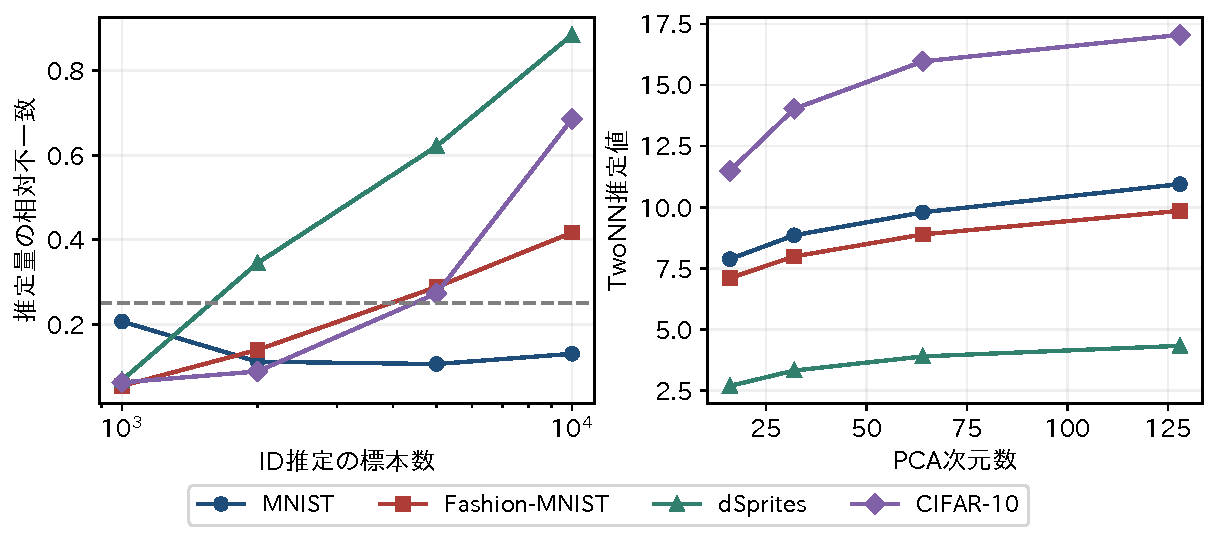
\includegraphics[width=\textwidth]{results/figures/NN53/id.pdf}
\caption{左：推定標本数を変えた生入力の$|d_{\rm TwoNN}-d_{\rm MLE}|/d_{\rm TwoNN}$。破線は0.25。右：PCA前処理後のTwoNN。PCA次元，標本数，表現は別の介入であり，AE結果は表\ref{tab:id}に示す。}
\label{fig:id}
\end{figure}

\subsection{正則化と品質条件への依存}\label{sec:beta}
手法$a$，データセット$d$について報告する変動幅を次式で定義する。
\begin{equation}
 S_{a,d}=\max_{\beta\in\mathcal B}\bar m_{a,d}(\beta)
         -\min_{\beta\in\mathcal B}\bar m_{a,d}(\beta),\qquad
 \bar m_{a,d}(\beta)=\frac15\sum_{s=1}^{5}m_{a,d,s}(\beta),
 \quad\mathcal B=\{0.25,0.5,1,2,4\}.
 \label{eq:span}
\end{equation}
これは返された未変換の次元数をシード間で平均した値の範囲であり，
シード内の変動幅を平均した値ではない。
FONDUE-VARの行では，未変換のゼロを含め，各設定で5個すべての出力が定義される。
検討した重み列に対する記述的な範囲であり，新たなパラメータ不要の頑健性指標ではない。

\begin{table}[H]
\caption{$\beta\in\{0.25,0.5,1,2,4\}$にわたる，返却次元数のシード平均の範囲。剪定変更実装は実装監査に限定する。固定32は設計上の定数であり，fallbackの変動幅はIDの頑健性ではない。dSpritesはベルヌーイ，他はガウス尤度。}\label{tab:span}
\small
\setlength{\tabcolsep}{3.5pt}
\begin{tabular*}{\textwidth}{@{\extracolsep{\fill}}lcccc@{}}
\toprule
手法 & MNIST & Fashion & dSprites & CIFAR-10 \\
\midrule
グリッド（MSE） & 14.8 & 20.8 & 40.0 & 91.2 \\
粗い探索 & 33.6 & 37.2 & 0.0 & 214.4 \\
固定32 & 0.0 & 0.0 & 0.0 & 0.0 \\
FONDUE & 3.8 & 0.8 & 0.8 & 8.8 \\
FONDUE-VAR（混合型保持） & 50.6 & 63.0 & 106.2 & 68.8 \\
昇順+$Q$ & 6.0 & 3.6 & 15.2 & 52.8 \\
FONDUE + Q & 3.6 & 1.6 & 28.0 & 44.8 \\
従来ID探索窓 & 6.0 & 37.2 & 0.0 & 214.4 \\
\bottomrule
\end{tabular*}
\end{table}

変動幅は手法とデータセットで異なり，大小関係は明確に逆転する。
例えば，昇順探索とFONDUE+$Q$の変動幅はMNISTで6.0と3.6，
dSpritesでは15.2と28.0である。
従来ID探索窓のCIFAR-10での214.4という変動幅はfallbackに由来する。
固定次元は設計上変動幅がゼロであり，
dSpritesのID fallbackも粗い探索が常に64を返すため変動幅がゼロになる。
どちらも選択の有用な頑健性を示さない。
尺度が異なるグリッド間で変動幅を平均せず，別条件へ移せる順位も主張しない。

ARDの呼出しでは選択段階の重みを変えておらず，
GECOでは$\beta$そのものではなくアンカー由来の制約を変えている。
両者は実装監査の対象であり，図\ref{fig:beta}の通常VAEの正則化比較には含めない。

\begin{figure}[!htbp]
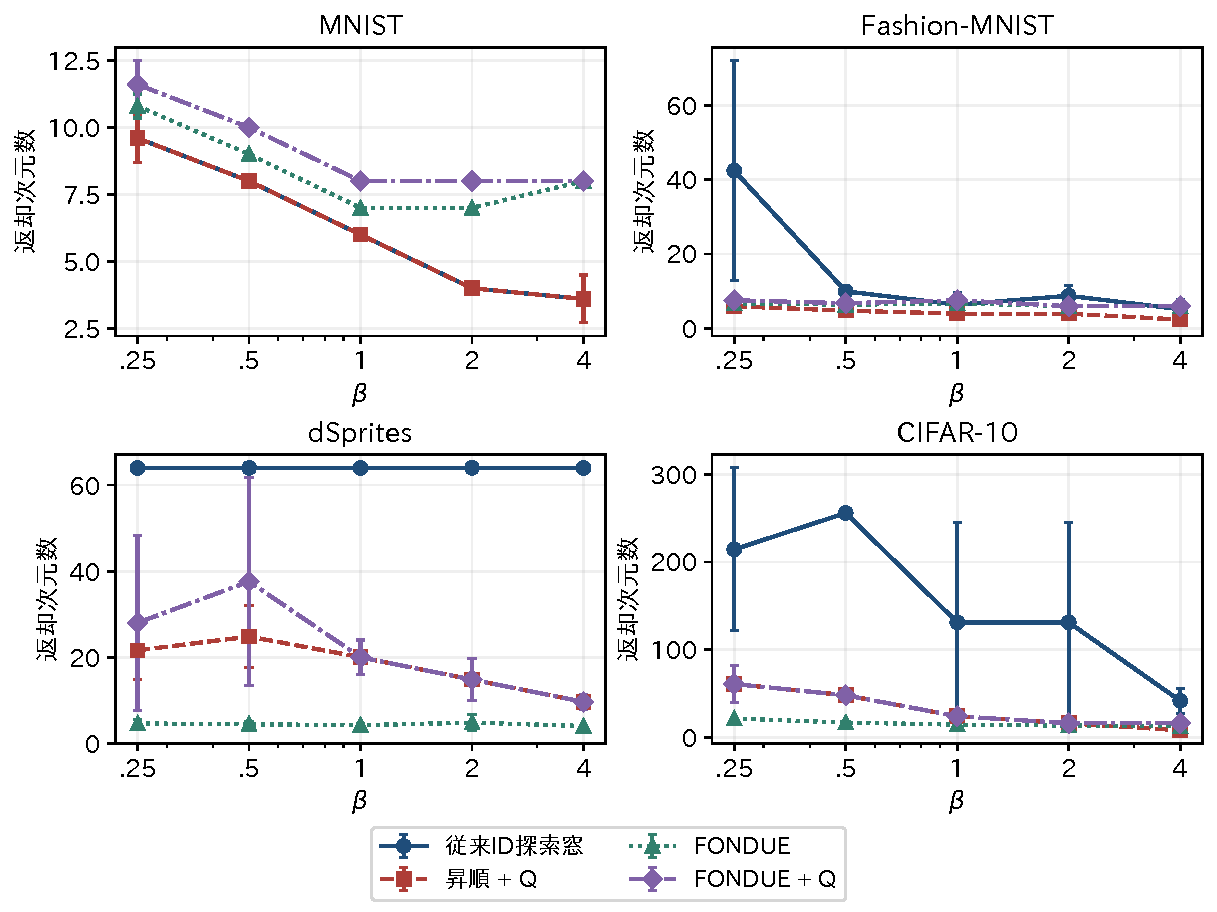
\includegraphics[width=\textwidth]{results/figures/NN53/beta.pdf}
\caption{5条件で返された未変換次元数。5候補シードの平均$\pm$SD。dSpritesはベルヌーイ，他はガウス尤度。これらの通常VAE選択器では学習時の$\beta$を変える。従来ID探索窓は，重み列全体でFashion-MNIST，dSprites，CIFAR-10にfallbackを用いる。}
\label{fig:beta}
\end{figure}

AU閾値への介入はcheckpointを固定して式\eqref{eq:au}を再計算する。
一方，品質許容幅への介入は，保存モデルのうちどれが目標を満たすかを変える。
いずれも学習時の$\beta$を変えることとは異なる。
これらの読み取り・品質解析は別に報告する（\ref{sec:au}節，付録\ref{app:sensitivity}）。
未検討のFONDUE停止閾値やARD累積関連度比率について，感度の主張は行わない。

\subsection{学習曲線，test評価，選択基準}
図\ref{fig:selectedcurves}は，主設定で昇順$Q$により選ばれた，
実際に早期停止した候補キャッシュの記録を用い，MNISTの6次元とCIFAR-10を含む。
各実行は記録されたepochまでを示し，proxyで選んだcheckpointに印を付ける。
これらのキャッシュには検証曲線だけがあり，epochごとの学習曲線はない。
欠けた学習測定値は補完しない。
別途行った新しいMNIST実行で，6次元の対応する学習・検証曲線を示す（付録\ref{app:newmodels}）。

\begin{figure}[!htbp]
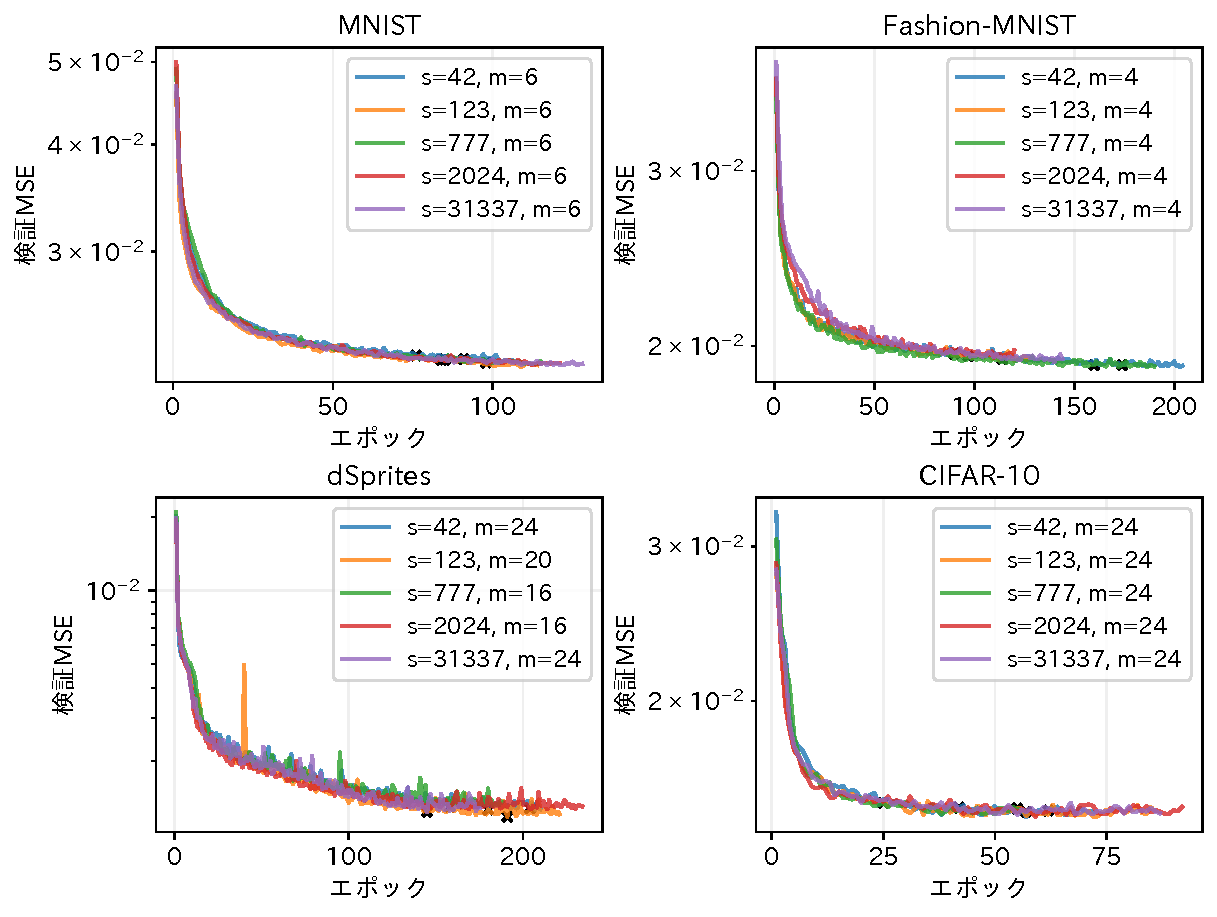
\includegraphics[width=\textwidth]{results/figures/NN53/selected_curves.pdf}
\caption{実際に選ばれた候補の検証MSE。$\beta=1$，5シード，dSpritesはベルヌーイ，他はガウス尤度。次元は昇順$Q$で選び，黒い十字はproxy選択epochを示す。曲線は記録上の停止時点で終わる。図\ref{fig:learning}の固定300 epochsの診断実行とは異なる。}
\label{fig:selectedcurves}
\end{figure}

保存された学習推移実験には，MNISTの12，32，64次元とdSpritesの6，16，32次元について，
各5シードの学習・検証曲線がある（図\ref{fig:learning}）。
学習MSEは，シード20260919で抽出した固定2000学習例の部分集合上で，決定論的モードにより評価する。
学習・検証の双方が改善するが，検証誤差の方が高い。
これら30実行のどれも，最終50 epochsの厳しいplateau判定を満たさない。
300 epochsの完了は収束の証明ではない。
この曲線は代表的な設定を対象とし，4データセットすべてを網羅しない。

\begin{figure}[!htbp]
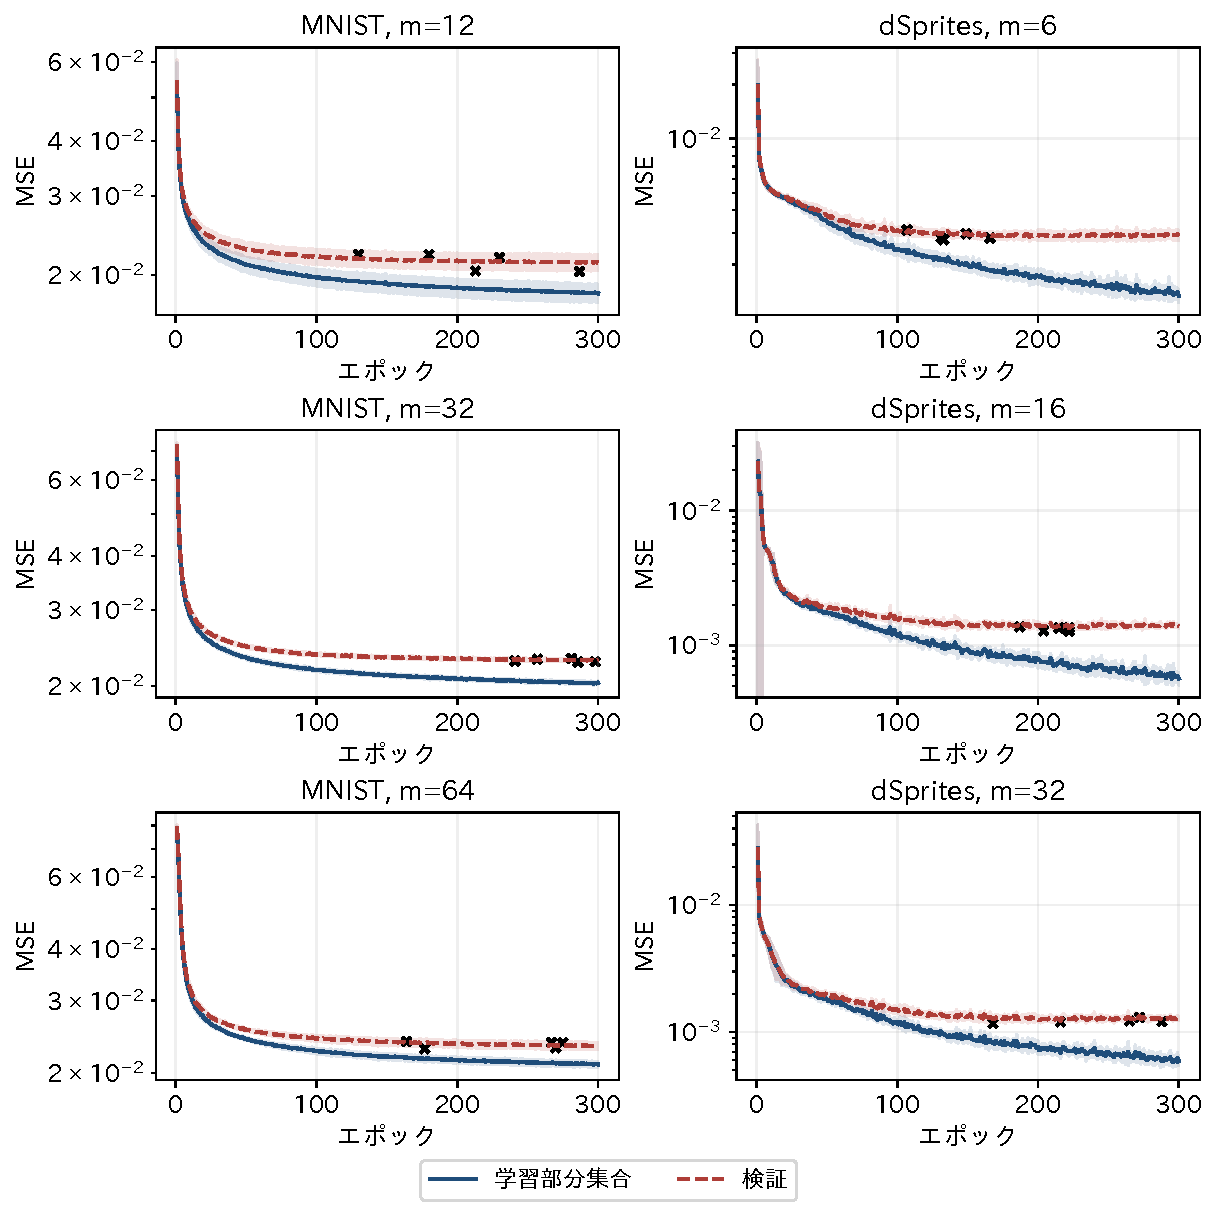
\includegraphics[width=\textwidth]{results/figures/NN53/learning.pdf}
\caption{学習・検証MSE。5シードの平均と$\pm$1 SD帯を示す。MNISTはガウス，dSpritesはベルヌーイ尤度，$\beta=1$。黒い十字は各実行の検証ELBO proxyで選んだcheckpoint。この診断実行には早期停止を用いない。}
\label{fig:learning}
\end{figure}

\clearpage
\begin{table}[H]
\caption{$\beta=1$，5シードでの選択基準比較。test MSEは$10^3$倍，プローブtest正解率は\%。プローブはクラスラベル（dSpritesでは形状）を使い，容量選択にも使うのはグリッド（プローブ）だけである。時間はアンカー補完を含む過去の記録であり，再評価の統一単価ではない。記録済みプローブ時間はその選択器に課す。他の表示プローブ正解率は補助評価であり，費用は加算していない。尤度は表\ref{tab:data}による。}\label{tab:selection}
\footnotesize
\setlength{\tabcolsep}{3.5pt}
\begin{tabular*}{\textwidth}{@{\extracolsep{\fill}}llcccc@{}}
\toprule
データセット & 基準 & $m$ & test MSE & 正解率 & 時間（秒） \\
\midrule
MNIST & グリッド（MSE） & $12.8 \pm 6.4$ & $20.50 \pm 0.26$ & $89.4 \pm 0.9$ & $628 \pm 35$ \\
MNIST & グリッド（ELBO proxy） & $10.0 \pm 2.0$ & $20.54 \pm 0.25$ & $89.3 \pm 0.7$ & $628 \pm 35$ \\
MNIST & グリッド（プローブ） & $51.2 \pm 13.4$ & $23.01 \pm 0.55$ & $92.7 \pm 0.5$ & $696 \pm 36$ \\
Fashion-MNIST & グリッド（MSE） & $22.8 \pm 15.6$ & $18.08 \pm 0.19$ & $75.5 \pm 2.6$ & $645 \pm 42$ \\
Fashion-MNIST & グリッド（ELBO proxy） & $15.6 \pm 8.0$ & $18.12 \pm 0.27$ & $74.4 \pm 2.6$ & $645 \pm 42$ \\
Fashion-MNIST & グリッド（プローブ） & $57.6 \pm 8.8$ & $18.99 \pm 0.46$ & $78.4 \pm 0.6$ & $750 \pm 40$ \\
dSprites & グリッド（MSE） & $57.6 \pm 14.3$ & $1.15 \pm 0.01$ & $47.7 \pm 2.3$ & $2565 \pm 82$ \\
dSprites & グリッド（ELBO proxy） & $57.6 \pm 14.3$ & $1.15 \pm 0.01$ & $47.7 \pm 2.3$ & $2565 \pm 82$ \\
dSprites & グリッド（プローブ） & $64.0 \pm 0.0$ & $1.16 \pm 0.03$ & $49.8 \pm 3.0$ & $2589 \pm 84$ \\
CIFAR-10 & グリッド（MSE） & $140.8 \pm 53.5$ & $14.07 \pm 0.04$ & $44.3 \pm 2.6$ & $428 \pm 16$ \\
CIFAR-10 & グリッド（ELBO proxy） & $192.0 \pm 45.3$ & $14.11 \pm 0.08$ & $46.1 \pm 1.1$ & $428 \pm 16$ \\
CIFAR-10 & グリッド（プローブ） & $256.0 \pm 0.0$ & $14.30 \pm 0.12$ & $47.3 \pm 1.0$ & $574 \pm 15$ \\
\bottomrule
\end{tabular*}
\end{table}

表\ref{tab:selection}に，以前は示していなかったMSE，ELBO proxy，線形プローブによるグリッド選択を示す。
目的が違えば，選択次元と再構成誤差も異なり得る。
プローブのtest正解率は補助的な教師ありの結果であり，教師なしの再構成品質を測るものではない。
この比較は同じ分割と保存候補を用い，ラベル付き検証データによる選択を明記している。

表\ref{tab:mcselection}の独立した新しいMNIST比較では，
\ref{sec:newvalidation}節の固定Monte Carlo手順により，実際の期待対数尤度を評価する。
保存済みMSEとKLから再構成した値ではない。
検証MSEは12次元，proxyは12次元，Monte Carlo ELBOも12次元を選ぶ。この実行での一致は，proxyがELBO推定量であることを意味しない。
全グリッドのスコア，MC誤差，選択epochを付録\ref{app:newmodels}に示す。
新しい学習シードが1つだけでは，いずれの基準についてもデータセット全体の優位性は確立できない。
\ref{sec:gpuvalidation}節で述べた評価コード上の理由から，
追加の4データセットの剪定記録は，このELBO容量選択比較を拡張するものではない。

\begin{table}[H]
\caption{新しいMNISTのシード42による容量選択。$\beta=1$，ガウス分散$1/2$。すべての基準が同じ12個のproxy選択checkpointから選ぶ。MSEは$10^3$倍，ELBOは例当たりの平均nats。$\pm$はMonte Carlo SE（$K=32$）であり，学習シード間SDではない。検証データによる選択を固定してからtestを評価する。}\label{tab:mcselection}
\small
\setlength{\tabcolsep}{3pt}
\begin{tabular*}{\textwidth}{@{\extracolsep{\fill}}lcccc@{}}
\toprule
基準 & 次元数 & 検証MSE & test MSE & MC ELBO $\pm$ MC SE \\
\midrule
MSE & 12 & 20.98 & 20.43 & $-478.067 \pm 0.012$ \\
ELBO proxy & 12 & 20.98 & 20.43 & $-478.067 \pm 0.012$ \\
MC ELBO & 12 & 20.98 & 20.43 & $-478.067 \pm 0.012$ \\
\bottomrule\end{tabular*}
\end{table}

\subsection{活性度の読み取り：推移，閾値，予測}\label{sec:au}
図\ref{fig:readouts}と表\ref{tab:readouts}は，同一checkpointで2種類の個数を比較する。
MNISTの64次元では，epoch 5の変数型による個数は$9.8\pm3.8$，AUは$49.4\pm8.1$であるが，
epoch 300ではいずれも$6.4\pm0.5$となる。
この例では，平均の一致とシード間の変動を区別できる。
表にはepoch 50から300までの同一実行内の変化も示す。
変化の大きさは条件に依存するため，最終値の一致から一般的な安定性の優位を推論しない。

\begin{table}[H]
\caption{変数型の個数$V$（活性型と混合型の和）とAU数$A$。5シード，$\beta=1$，MNISTはガウス，dSpritesはベルヌーイ尤度。平均$\pm$SDはシード間変動を表す。最終列は$V/A$についてepoch 50から300までの実行内絶対変化の平均であり，時間方向の分散ではない。}\label{tab:readouts}
\footnotesize
\setlength{\tabcolsep}{3.5pt}
\begin{tabular*}{\textwidth}{@{\extracolsep{\fill}}lcccccc@{}}
\toprule
データセット & $m$ & $V_5$ & $A_5$ & $V_{300}$ & $A_{300}$ & 変化 \\
\midrule
MNIST & 12 & $7.2 \pm 0.8$ & $8.0 \pm 1.6$ & $6.4 \pm 0.5$ & $6.4 \pm 0.5$ & 0.0/0.0 \\
MNIST & 32 & $8.2 \pm 1.5$ & $20.8 \pm 4.2$ & $6.0 \pm 0.0$ & $6.0 \pm 0.0$ & 0.0/0.0 \\
MNIST & 64 & $9.8 \pm 3.8$ & $49.4 \pm 8.1$ & $6.4 \pm 0.5$ & $6.4 \pm 0.5$ & 0.4/2.6 \\
dSprites & 6 & $6.0 \pm 0.0$ & $6.0 \pm 0.0$ & $6.0 \pm 0.0$ & $6.0 \pm 0.0$ & 0.0/0.0 \\
dSprites & 16 & $16.0 \pm 0.0$ & $16.0 \pm 0.0$ & $14.2 \pm 0.4$ & $13.4 \pm 0.5$ & 1.8/1.8 \\
dSprites & 32 & $32.0 \pm 0.0$ & $31.8 \pm 0.4$ & $14.2 \pm 1.1$ & $14.4 \pm 1.1$ & 12.4/4.2 \\
\bottomrule
\end{tabular*}
\end{table}

\begin{figure}[!htbp]
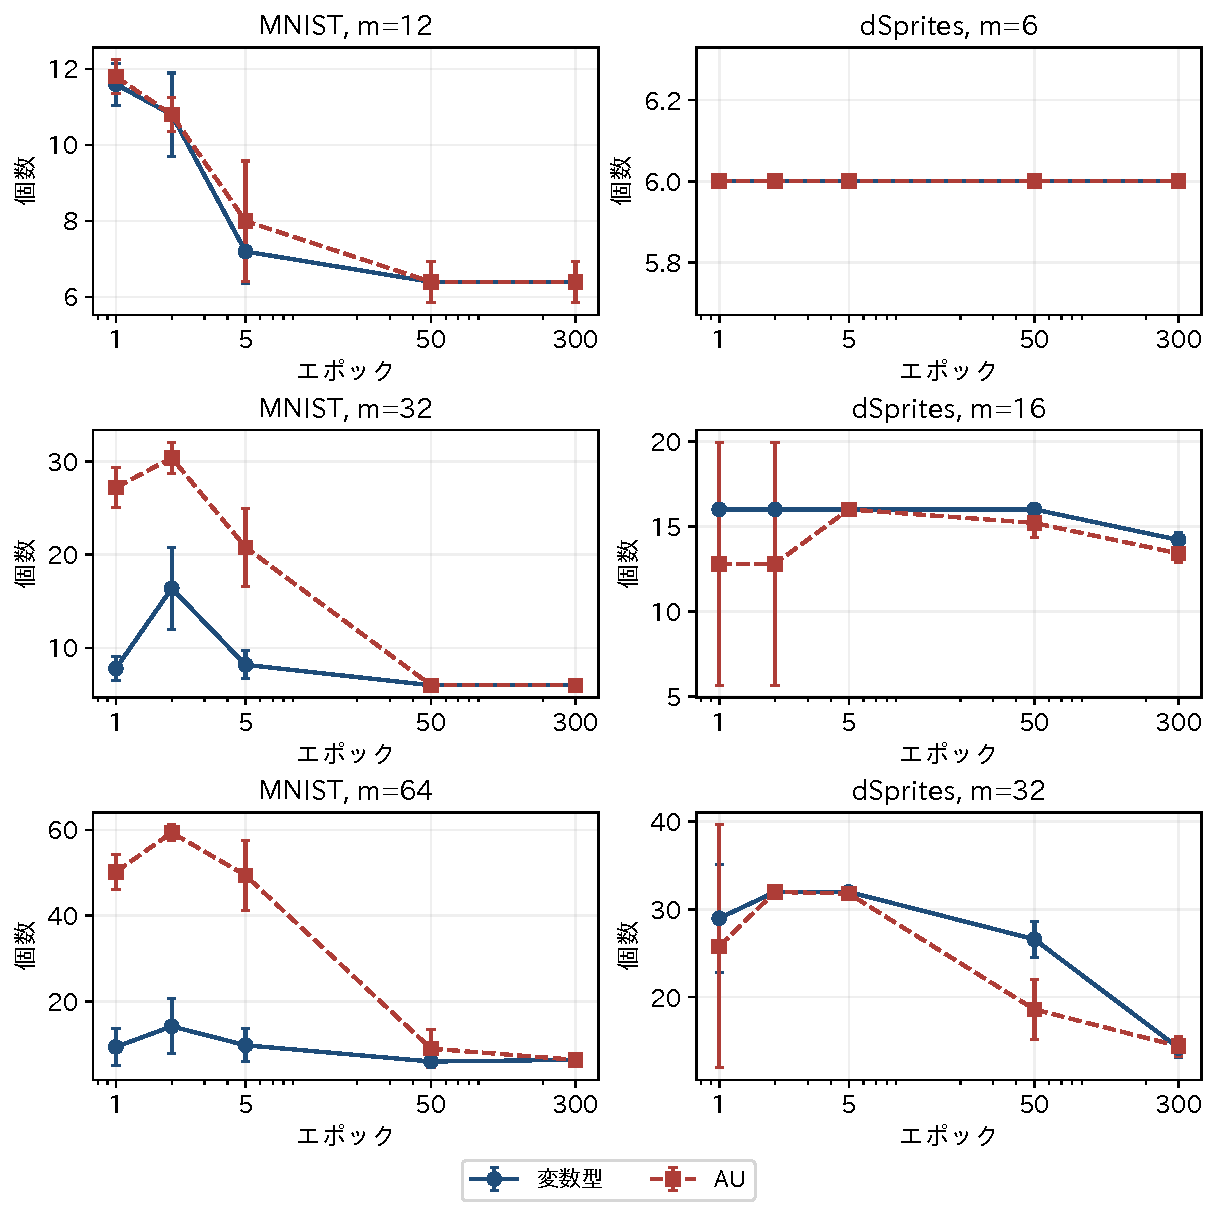
\includegraphics[width=\textwidth]{results/figures/NN53/readouts.pdf}
\caption{epoch 1，2，5，50，300の同一checkpointから得た変数型の個数（活性型と混合型の和）とAU。平均とシードSDを示し，線は観測されたcheckpoint間だけを結ぶ。$\beta=1$，MNISTはガウス，dSpritesはベルヌーイ尤度。全容量に等しい個数が一定でも，診断の安定性の証拠にはならない。}
\label{fig:readouts}
\end{figure}

図\ref{fig:delta}の閾値だけを変える比較では，$\beta=1$のcheckpointを固定する。
CIFAR-10では，$\delta=0.001$は検討したすべてのグリッド次元で全座標を数えるが，
$\delta=0.1$は大きな容量で数える座標がはるかに少ない。
したがって「未使用座標がない」という推論はこの閾値に依存する。
閾値の正規化は診断の定義を変えるものであり，次元推定を確立するものではない。

\begin{figure}[!htbp]
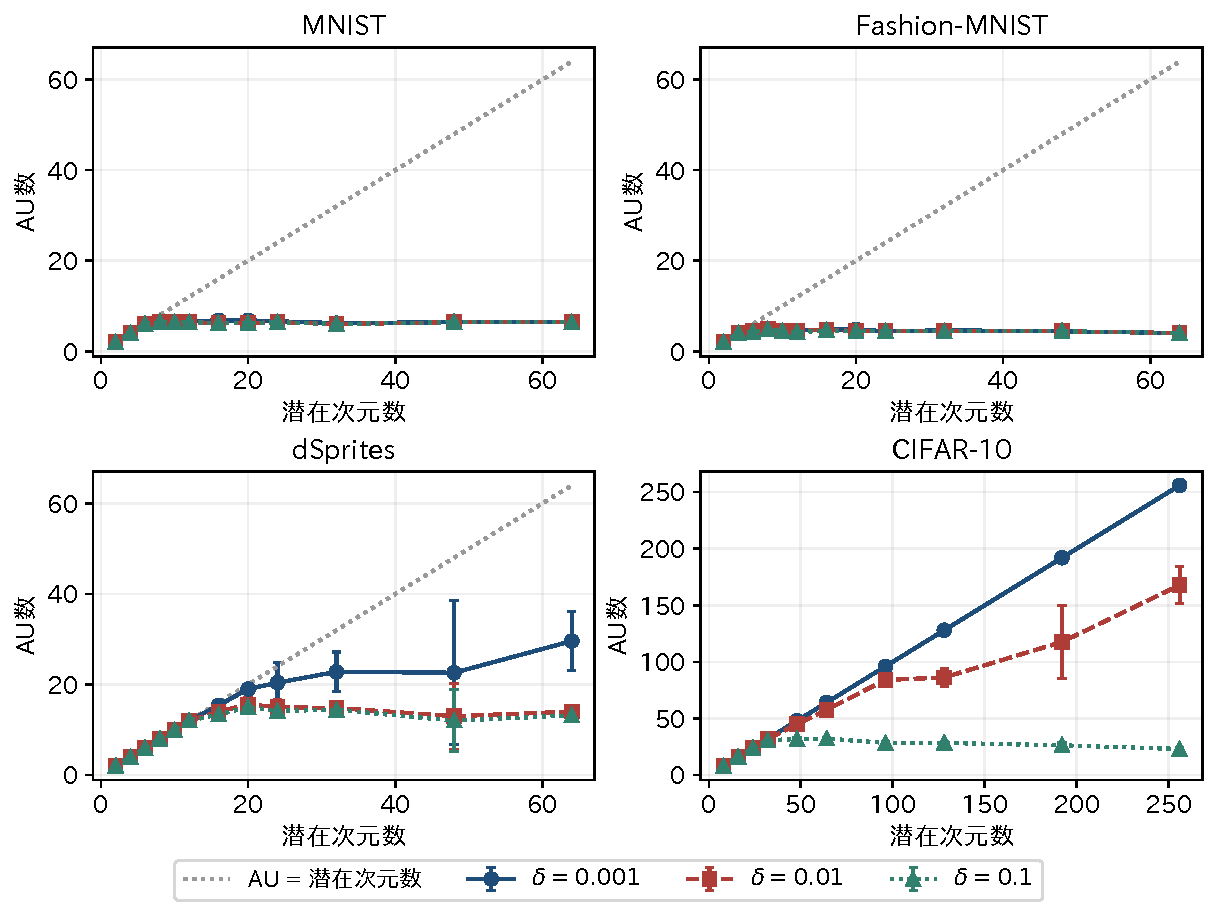
\includegraphics[width=\textwidth]{results/figures/NN53/delta.pdf}
\caption{同じ$\beta=1$候補に対する3閾値でのAU。平均$\pm$シードSD。dSpritesはベルヌーイ，他はガウス尤度。対角線は容量である。これは読み取り閾値への介入であり，図\ref{fig:beta}の学習・条件への介入とは異なる。}
\label{fig:delta}
\end{figure}

予測課題は，1つ小さいグリッド候補が，同じシードの品質目標を満たすかを判定することである。
各行は，最小グリッド次元以外の容量で検証データにより選ばれた1個のcheckpointである。
基準特徴量は，検証MSE，KL，ELBO proxy，次元数，次元数と入力IDの比，
直近20記録epochsの検証MSEの傾きである。
追加する3つのAU特徴量は，AU，AU/次元数，AU/入力IDとする。
標準化は開発用の行だけで適合する。
$L_2$ロジスティック予測器をMNISTの55行に適合し，
開発データを3シードと2シードに分けて$C=10$を選ぶ。
評価はdSpritesの55行，Fashion-MNISTの55行，CIFAR-10の45行で行い，各5シードを用いる。
設定されていたMNIST-CNNの予測条件は実行していない。

開発用分割ではシード42，123，777で内部適合を行い，2024，31337で$C$を選んだ後，5シードすべてで再適合する。
予測器の最大反復数は5000とする。
各評価データセット・シードのブロックは，そのシードの最小次元を除く全グリッド次元で採点する。
checkpointの各行を独立な観測として再標本化しない。

当初の内部仕様に基づく解析では，AUを追加した予測器と基準予測器のAUROC差は$+0.108$であり，
シード記録を用いた2000回のbootstrapの95\%区間は$[+0.059,+0.157]$と報告されていた。
後から追加した対照は，独立な3個の標準正規特徴量と1つの雑音実現（生成器シード7）を用い，
その改善量は別に$+0.098$，区間は$[-0.025,+0.227]$と報告された。
これらの区間の重なりは，両者の差の検定でも同等性の証明でもない。
これらの保存値は元の解析の記録として残すが，妥当性が確認された正の所見とは扱わない。
そのAUROC計算は，データセット間の分布変化により数値的に飽和し得る確率値を用いていた。

\begin{table}[H]
\caption{$\beta=1$の対応付きAU事後比較。飽和確率の同順位を避けるためロジスティック決定スコアを用いる。各値は，各シードの最小次元を除く全容量で評価したAUROCを5シードで平均したもの。無作為特徴量は生成器シード7の標準正規乱数3列。全手法が同じ行とラベルを用いる。}\label{tab:au}
\footnotesize
\setlength{\tabcolsep}{3.5pt}
\begin{tabular*}{\textwidth}{@{\extracolsep{\fill}}lccccc@{}}
\toprule
評価条件 & 行数 & 基準 & 基準+AU & 基準+無作為 & AU$-$無作為 \\
\midrule
dSprites & 55 & 0.950 & 0.858 & 0.898 & -0.041 \\
Fashion-MNIST & 55 & 0.980 & 1.000 & 0.880 & +0.120 \\
CIFAR-10 & 45 & 1.000 & 1.000 & 1.000 & +0.000 \\
\bottomrule
\end{tabular*}
\end{table}

基準AUROCは既に，dSpritesで0.950，Fashion-MNISTで0.980，CIFAR-10で1.000である。
特にCIFAR-10にはAUROCを上げる余地がない。
この結果は，特定の天井に近い予測課題での追加価値に関するものであり，AU一般の情報量を論じるものではない。

本改訂では$\beta=1$を明示的に固定し，対象行を宣言されたグリッドに限定して両予測器を再構成し，
ロジスティック回帰の決定スコアからAUROCを計算する。
元のキャッシュ読出し処理には$\beta$のフィルタもグリッドの制限もなく，
キャッシュ拡張後に再実行すると対象行も曖昧になる。
決定スコアは，sigmoid確率がちょうど1へ丸められると失われる順位を保持する。
飽和件数は付録\ref{app:sensitivity}に示す。
これは修正した事後解析であり，保存されていた確率の厳密な再現ではない。
AU追加から基準を引いた差は$-0.024$，区間は$[-0.102,+0.027]$となる。
AU予測器と無作為特徴量予測器も，同じデータセット・シードのブロックで比較する。
対応差の平均は$+0.026$であり，事後的な階層bootstrapの95\%区間は
$[-0.040,+0.133]$である（2000反復）。
各反復では，3評価データセットを再標本化し，選ばれたデータセット内で5シードブロックを再標本化する。
ブロック内の全容量と両予測器の対応は保持する。
モデルは固定するため，この区間は開発モデルの適合に関する不確実性を含まない。
評価データセットは3つしかなく，条件をまたぐ推論の精度は限られる。
補助解析では100個の雑音実現（シード0--99）で対照を平均し，
同じ再標本化で対応差$-0.007$，区間$[-0.064,+0.039]$を得た。
どちらの解析も，これらの評価条件でAU固有の利得を確立しない。
AUに情報がない，両予測器が同等である，あるいは有意差がないことが検出力不足を証明する，とは主張しない。

\subsection{実装監査と退化出力}
過去の損失尺度の修正を付録\ref{app:scaling}に記す。
現在の画像比較は，潜在次元について和を取る修正後の規約を用いる。

ARMに固有の追加実装検査は，平均を取る順序に関するものである。
提供された線形損失の検査では，各例の対立標本を使う推定量を解析勾配と比較する。
ゲート標本との相関を構成する前に損失を平均すると，必要な対応が失われる。
追加の学習コードは各例の損失を用いる。
この構成要素の修正は，すべての制約が満たされることを意味しない。
最終時点の件数を表\ref{tab:armnew}に示す。
これは，過去の損失尺度とARD関連度正規化の監査とは別の問題である。

FONDUE-VARの活性型のみを残す設定がゼロを返すことは，別の現象であり，3件目の和・平均の欠陥ではない。
MNISTの1 epoch設定では5試行すべてがゼロを返し，最終VAEは存在しない。
表\ref{tab:var}に両設定と品質・有効モデルの件数を示す。

\begin{table}[H]
\caption{$\beta=1$のFONDUE-VAR。混合型保持の両設定，有効モデル数，品質達成数，test MSE（$10^3$倍），記録学習時間。未変換のゼロ出力も次元集計に残すが，モデルが存在しない場合にMSEはない。5シード，尤度は表\ref{tab:data}による。}\label{tab:var}
\footnotesize
\setlength{\tabcolsep}{3.5pt}
\begin{tabular*}{\textwidth}{@{\extracolsep{\fill}}lcccccc@{}}
\toprule
データセット & 混合型保持 & 未変換$m$ & 有効 & $Q$ & test MSE & 時間（秒） \\
\midrule
MNIST & はい & $9.8 \pm 8.5$ & 5/5 & 5/5 & $22.53 \pm 0.89$ & $113 \pm 22$ \\
MNIST & いいえ & $0.0 \pm 0.0$ & 0/5 & 0/5 & --- & $63 \pm 10$ \\
Fashion-MNIST & はい & $14.4 \pm 3.8$ & 5/5 & 5/5 & $18.96 \pm 0.39$ & $91 \pm 11$ \\
Fashion-MNIST & いいえ & $2.0 \pm 0.0$ & 5/5 & 0/5 & $25.27 \pm 0.06$ & $120 \pm 18$ \\
dSprites & はい & $26.0 \pm 49.5$ & 4/5 & 1/5 & $9.53 \pm 9.62$ & $412 \pm 118$ \\
dSprites & いいえ & $1.2 \pm 1.6$ & 2/5 & 0/5 & $7.71 \pm 0.02$ & $278 \pm 49$ \\
CIFAR-10 & はい & $34.2 \pm 1.3$ & 5/5 & 5/5 & $14.40 \pm 0.15$ & $103 \pm 13$ \\
CIFAR-10 & いいえ & $3.2 \pm 0.8$ & 5/5 & 0/5 & $31.65 \pm 2.68$ & $96 \pm 13$ \\
\bottomrule
\end{tabular*}
\end{table}

\section{考察}\label{sec:discussion}
開始次元数を統制したアブレーションにより，ID-localの結果の解釈が変わる。
同じfallbackを持つID-gated midpointでも，最小次元との100/100の一致が再現される。
IDを採用した25条件では，ID開始点は答えを変えずにより多くの候補を要求する。
参照群を使わない中点方策の2件の誤りは，ID方策が昇順fallbackを使う条件で起こる。
したがって，この証拠からID由来の開始次元数の優位性は確立できない。
信頼性判定を備えた探索が有効かという仮説と，
幾何学情報が有用な開始次元数を与えるかという仮説は別である。

目標には最大次元のアンカーが含まれるため，
保存グリッド内で上方へ網羅的に探索すれば品質達成は保証される。
一方，最小性と費用は実質的な評価対象として残る。
全組合せ解析では10,000設定中155件で非最小の出力が得られ，
既定値での一致は局所探索の普遍的な保証ではない。
共有参照群，単一の分割，事後的な方策設計，4データセットという範囲が推論を制限する。
独立した参照群での追試は未実施である。
取得費用と再利用費用も，異なる利用状況に対応する。

正則化に伴う変動範囲とAU閾値への応答は，異なる介入を測定している。
次元の変動には，fallback，グリッド尺度，品質目標の変化を反映するものがある。
一定の出力は，設計上の固定値や変化させていない実装引数によって生じ得る。
対応付き予測比較では，天井に近い課題において，
対応する無作為特徴量対照に対するAU固有の優位性は確立されない。
したがって本研究でのAUの役割は，明示した閾値のもとで座標の利用状況を診断することに限定される。

native剪定の比較は，選択個数と，保持軸を用いるモデルの再構成を別々に評価する必要性を示す。
ローカルな標本中心のARD変種は，MNISTとFashion-MNISTではマスク後の平均MSEをほぼ維持する一方，
dSpritesでは大きく悪化し，復号器微調整による回復も部分的である。
全次元モデル自体がすでに$Q$に届かないため，dSpritesの4条件のいずれも，
目標品質を維持した圧縮の成功として示すことはできない。
マスクは元のネットワークにおける推論規則の検証であり，パラメータ数，メモリ，遅延の削減を測定したものではない。
固定微調整予算は追加学習を要し，それまで事前分布更新専用だったプールも用いる。
マスクなしで30 epochs微調整する対照は実施していないため，改善をマスクの影響の補償だけに帰属できない。

これらの結果は，各データセット3シードへnative品質の根拠を広げるが，ローカルな学習設定を維持している。
厳密ヤコビアンは有限刻み幅近似を除くもので，標本から求めた関連度スコアや学習表現の不確実性を除くものではない。
Gaussian KL近似はARD原著と共通である。
標本中心の分散更新は引き続き感度検証用の変種であり，原著のゼロ中心設定に必要な修正ではない。
この変種の結果をすべてのARD設定へ一般化したり，原著手法の厳密なbenchmarkとして扱ったりすることはできない。

追加された4データセットのELBOフィールドは，
主張する量に必要な期待尤度とnativeの事前分布に対するKLを計算していない。
妥当なMC ELBOによる容量選択の証拠は，
MNISTの1シードとproxyで選んだcheckpointに留まる。
同様に，新しい剪定曲線は欠けている過去の通常VAE学習曲線を回復しない。
原著アルゴリズム全体の再現，独立参照群による検証，
完全なend-to-end時間計測，情報漏洩のない合成データの分離評価は未完了である。
合成データ診断（付録\ref{app:synthetic}）は尺度と座標の効果を記述するもので，
位相が活性軸数を決めることを示さない。

\section{結論}\label{sec:conclusion}
明示的な品質・費用の定義の下で，内在次元誘導によるVAEボトルネック選択と活性ユニット診断を評価した。
信頼性判定，fallback，参照費用を固定すると，IDが採用されるのはMNISTの25条件だけである。
ID由来の開始点と判定付き中点は，平均8.84件と5.84件の要求で同じ次元数を選ぶ。
他の75条件は同じ昇順fallbackを用いる。
局所探索の最小性は，信頼性と係数の設定にも依存する。
追加剪定実験では，native品質，次元転用後の品質，学習制約を区別する。
ローカルな標本中心のARD変種では，選択軸によるマスク後も2データセットの再構成はほぼ変わらないが，
dSpritesのMSEは126.3\%増える。
復号器微調整による回復は部分的であり，dSpritesの4条件すべてが$Q$に届かない。
AUは，今回の天井に近い課題で追加の予測価値を確立しない。
本研究の貢献はID誘導と潜在診断の限定的な評価であり，一般的な効率上の優位性や剪定品質の保証を確立するものではない。

\paragraph{著者の貢献}
構想：C.O.，M.D.，K.J.；方法論：C.O.，K.J.；ソフトウェア：C.O.，M.D.；
検証：C.O.，M.D.，K.J.；形式的解析：C.O.，K.J.；調査：C.O.，M.D.，K.J.；
初稿執筆：C.O.，K.J.；原稿の検討・編集：C.O.，M.D.，K.J.；
監督・プロジェクト管理：K.J.
\paragraph{研究助成}
本研究は，JSPS科研費JP24K15115およびJP26K14984，
東京都市大学重点研究［知能技術最適化研究ユニット：ORBIT］，
東北大学電気通信研究所の共同研究プロジェクト，
ならびに電気通信普及財団（TAF）の研究助成を受けた。
\paragraph{倫理審査}該当なし。
\paragraph{インフォームド・コンセント}該当なし。
\paragraph{データの利用可能性}
画像データセットは引用した配布元から公開されている。
同梱の査読用補足資料\texttt{MAKE53\_reproducibility.zip}には，
設定，過去および追加の結果記録，解析・学習コード，分割添字，
図，独立したMNIST検証のcheckpoint，SHA-256 manifestを含む。
アーカイブを展開して\texttt{README.md}に従うこと。
付録\ref{app:inventory}に内容の対応を示す。
過去のMAKE49および追加MAKE52剪定実験のcheckpointは利用できない。
アーカイブは本改訂に添付するもので，公開データ寄託ではなくDOIもない。
\paragraph{謝辞}
従来の原稿作成では，実験コードの草案・整理と英文編集に生成AIの支援を用いた。
今回の記録監査，再集計，モデル検証結果の解析，図の作成，原稿改訂ではOpenAI Codexの支援を用いた。
科学的内容の責任は著者らにある。
\paragraph{利益相反}著者らは利益相反がないことを宣言する。

\clearpage
\appendix
\section{品質目標と結果の計上}\label{app:targets}
\begin{table}[H]
\caption{品質アンカーと目標。MSEの単位は$10^{-3}$，5シードの平均$\pm$SD。各判定は表示平均ではなく，そのシード固有の目標を用いる。相対許容幅は10\%で，絶対下限は有効にならない。dSpritesはベルヌーイ，他はガウス尤度。}\label{tab:anchors}
\small
\setlength{\tabcolsep}{3.5pt}
\begin{tabular*}{\textwidth}{@{\extracolsep{\fill}}lccc@{}}
\toprule
データセット & $\beta$ & アンカーMSE & 目標$T_{D,s}$ \\
\midrule
MNIST & 0.25 & $15.843 \pm 0.562$ & $17.428 \pm 0.618$ \\
MNIST & 0.5 & $19.202 \pm 0.497$ & $21.122 \pm 0.546$ \\
MNIST & 1 & $23.712 \pm 0.532$ & $26.084 \pm 0.585$ \\
MNIST & 2 & $30.061 \pm 0.560$ & $33.068 \pm 0.617$ \\
MNIST & 4 & $38.977 \pm 0.673$ & $42.875 \pm 0.740$ \\
Fashion-MNIST & 0.25 & $15.591 \pm 0.678$ & $17.150 \pm 0.746$ \\
Fashion-MNIST & 0.5 & $17.408 \pm 0.513$ & $19.148 \pm 0.564$ \\
Fashion-MNIST & 1 & $19.679 \pm 0.162$ & $21.647 \pm 0.179$ \\
Fashion-MNIST & 2 & $22.416 \pm 0.527$ & $24.658 \pm 0.580$ \\
Fashion-MNIST & 4 & $25.967 \pm 0.587$ & $28.564 \pm 0.645$ \\
dSprites & 0.25 & $1.015 \pm 0.032$ & $1.117 \pm 0.036$ \\
dSprites & 0.5 & $1.040 \pm 0.032$ & $1.144 \pm 0.035$ \\
dSprites & 1 & $1.170 \pm 0.024$ & $1.287 \pm 0.026$ \\
dSprites & 2 & $1.453 \pm 0.038$ & $1.598 \pm 0.041$ \\
dSprites & 4 & $2.144 \pm 0.064$ & $2.358 \pm 0.070$ \\
CIFAR-10 & 0.25 & $9.407 \pm 0.610$ & $10.348 \pm 0.671$ \\
CIFAR-10 & 0.5 & $11.151 \pm 0.200$ & $12.266 \pm 0.220$ \\
CIFAR-10 & 1 & $14.064 \pm 0.108$ & $15.470 \pm 0.119$ \\
CIFAR-10 & 2 & $17.806 \pm 0.262$ & $19.587 \pm 0.288$ \\
CIFAR-10 & 4 & $22.399 \pm 0.286$ & $24.638 \pm 0.314$ \\
\bottomrule
\end{tabular*}
\end{table}

\subsection{各状態の独立した集計}\label{app:outcomes}
以下の表は，元の複合状態と，各フラグおよび最終モデルの品質を分ける。
予算フラグはID fallbackと同時に立ち得る。
剪定用ラッパーは学習中に通常選択器の予算を強制していないため，
予算フラグがゼロであることは同じ予算管理の証拠ではない。
予算超過試行を含め，有効な返却モデルはすべて主設定の平均に含める。
退化出力は未変換個数と費用の要約に含めるが，MSEには含めない。
\begin{table}[H]
\caption{$\beta=1$の結果監査。すべて5試行中の件数。S：記録上の成功；I：ID信頼性不足；B：予算超過；D：退化；N：小容量の代替なし。FBはfallbackフラグ。予算，検証品質$Q$，最終VAEの小容量化は，それぞれ独立に再計算するかフラグから読み取る。}\label{tab:outcomes0}
\footnotesize
\setlength{\tabcolsep}{3.5pt}
\begin{tabular*}{\textwidth}{@{\extracolsep{\fill}}llccccc@{}}
\toprule
データセット & 手法 & 状態 & FB & 予算超過 & $Q$ & 小容量化 \\
\midrule
MNIST & グリッド（MSE） & S5 & 0 & 0 & 5 & 5 \\
MNIST & FONDUE & S5 & 0 & 0 & 5 & 5 \\
MNIST & FONDUE + Q & S5 & 0 & 0 & 5 & 5 \\
MNIST & GECO変更実装 & S5 & 0 & 0 & 5 & 5 \\
MNIST & ARD変更実装 & S5 & 0 & 0 & 5 & 5 \\
MNIST & 昇順+$Q$ & S5 & 0 & 0 & 5 & 5 \\
MNIST & 従来ID探索窓 & S5 & 0 & 0 & 5 & 5 \\
MNIST & FONDUE-VAR（混合型保持） & S5 & 0 & 0 & 5 & 5 \\
MNIST & FONDUE-VAR（活性型のみ） & D5 & 0 & 0 & 0 & 0 \\
Fashion-MNIST & グリッド（MSE） & S5 & 0 & 0 & 5 & 5 \\
Fashion-MNIST & FONDUE & S5 & 0 & 0 & 5 & 5 \\
Fashion-MNIST & FONDUE + Q & S5 & 0 & 0 & 5 & 5 \\
Fashion-MNIST & GECO変更実装 & S5 & 0 & 0 & 5 & 5 \\
Fashion-MNIST & ARD変更実装 & S5 & 0 & 0 & 4 & 5 \\
Fashion-MNIST & 昇順+$Q$ & S5 & 0 & 0 & 5 & 5 \\
Fashion-MNIST & 従来ID探索窓 & I5 & 5 & 0 & 5 & 5 \\
Fashion-MNIST & FONDUE-VAR（混合型保持） & S5 & 0 & 0 & 5 & 5 \\
Fashion-MNIST & FONDUE-VAR（活性型のみ） & S5 & 0 & 0 & 0 & 5 \\
\bottomrule
\end{tabular*}
\end{table}
\begin{table}[H]
\caption{$\beta=1$の結果監査。すべて5試行中の件数。S：記録上の成功；I：ID信頼性不足；B：予算超過；D：退化；N：小容量の代替なし。FBはfallbackフラグ。予算，検証品質$Q$，最終VAEの小容量化は，それぞれ独立に再計算するかフラグから読み取る。}\label{tab:outcomes1}
\footnotesize
\setlength{\tabcolsep}{3.5pt}
\begin{tabular*}{\textwidth}{@{\extracolsep{\fill}}llccccc@{}}
\toprule
データセット & 手法 & 状態 & FB & 予算超過 & $Q$ & 小容量化 \\
\midrule
dSprites & グリッド（MSE） & S5 & 0 & 0 & 5 & 1 \\
dSprites & FONDUE & S5 & 0 & 0 & 0 & 5 \\
dSprites & FONDUE + Q & B1, S4 & 0 & 1 & 5 & 5 \\
dSprites & GECO変更実装 & S5 & 0 & 0 & 5 & 0 \\
dSprites & ARD変更実装 & S5 & 0 & 0 & 0 & 5 \\
dSprites & 昇順+$Q$ & S5 & 0 & 0 & 5 & 5 \\
dSprites & 従来ID探索窓 & I5 & 5 & 0 & 5 & 0 \\
dSprites & FONDUE-VAR（混合型保持） & D1, S4 & 0 & 0 & 1 & 3 \\
dSprites & FONDUE-VAR（活性型のみ） & D3, S2 & 0 & 0 & 0 & 2 \\
CIFAR-10 & グリッド（MSE） & S5 & 0 & 0 & 5 & 5 \\
CIFAR-10 & FONDUE & S5 & 0 & 0 & 0 & 5 \\
CIFAR-10 & FONDUE + Q & S5 & 0 & 0 & 5 & 5 \\
CIFAR-10 & GECO変更実装 & S5 & 0 & 0 & 2 & 5 \\
CIFAR-10 & ARD変更実装 & S5 & 0 & 0 & 0 & 5 \\
CIFAR-10 & 昇順+$Q$ & S5 & 0 & 0 & 5 & 5 \\
CIFAR-10 & 従来ID探索窓 & I5 & 5 & 0 & 5 & 3 \\
CIFAR-10 & FONDUE-VAR（混合型保持） & S5 & 0 & 0 & 5 & 5 \\
CIFAR-10 & FONDUE-VAR（活性型のみ） & S5 & 0 & 0 & 0 & 5 \\
\bottomrule
\end{tabular*}
\end{table}

\section{探索感度と時間記録の来歴}\label{app:search}
これらの表は，アルゴリズム\ref{alg:replay}の事後的な方策を用いる。
元の実験を定義し直すものではない。
\begin{table}[H]
\caption{$\beta=1$，$R\le0.15$，$A\le0.25$でのID-local再評価の係数感度。5係数すべてを示し，棄却されたデータセットは同じ昇順fallbackを使う。5シード，尤度は表\ref{tab:data}による。}\label{tab:coefficient}
\small
\setlength{\tabcolsep}{3pt}
\begin{tabular*}{\textwidth}{@{\extracolsep{\fill}}lcccccc@{}}
\toprule
データセット & $c$ & 次元数 & $Q$ & 一致 & 要求数 & 初回費用（秒） \\
\midrule
MNIST & 1 & $6.0 \pm 0.0$ & 5/5 & 5/5 & 6.0 & 487 \\
MNIST & 1.5 & $6.0 \pm 0.0$ & 5/5 & 5/5 & 8.0 & 584 \\
MNIST & 2 & $6.0 \pm 0.0$ & 5/5 & 5/5 & 9.0 & 636 \\
MNIST & 3 & $6.0 \pm 0.0$ & 5/5 & 5/5 & 11.0 & 743 \\
MNIST & 4 & $6.0 \pm 0.0$ & 5/5 & 5/5 & 11.0 & 743 \\
Fashion-MNIST & 1 & $4.0 \pm 0.0$ & 5/5 & 5/5 & 3.0 & 416 \\
Fashion-MNIST & 1.5 & $4.0 \pm 0.0$ & 5/5 & 5/5 & 3.0 & 416 \\
Fashion-MNIST & 2 & $4.0 \pm 0.0$ & 5/5 & 5/5 & 3.0 & 416 \\
Fashion-MNIST & 3 & $4.0 \pm 0.0$ & 5/5 & 5/5 & 3.0 & 416 \\
Fashion-MNIST & 4 & $4.0 \pm 0.0$ & 5/5 & 5/5 & 3.0 & 416 \\
dSprites & 1 & $20.0 \pm 4.0$ & 5/5 & 5/5 & 9.0 & 2092 \\
dSprites & 1.5 & $20.0 \pm 4.0$ & 5/5 & 5/5 & 9.0 & 2092 \\
dSprites & 2 & $20.0 \pm 4.0$ & 5/5 & 5/5 & 9.0 & 2092 \\
dSprites & 3 & $20.0 \pm 4.0$ & 5/5 & 5/5 & 9.0 & 2092 \\
dSprites & 4 & $20.0 \pm 4.0$ & 5/5 & 5/5 & 9.0 & 2092 \\
CIFAR-10 & 1 & $24.0 \pm 0.0$ & 5/5 & 5/5 & 4.0 & 498 \\
CIFAR-10 & 1.5 & $24.0 \pm 0.0$ & 5/5 & 5/5 & 4.0 & 498 \\
CIFAR-10 & 2 & $24.0 \pm 0.0$ & 5/5 & 5/5 & 4.0 & 498 \\
CIFAR-10 & 3 & $24.0 \pm 0.0$ & 5/5 & 5/5 & 4.0 & 498 \\
CIFAR-10 & 4 & $24.0 \pm 0.0$ & 5/5 & 5/5 & 4.0 & 498 \\
\bottomrule\end{tabular*}
\end{table}
\begin{table}[H]
\caption{$\beta=1$，$c=2$での信頼性閾値感度。ID：IDを開始点とする局所探索；FB：昇順fallback。極端な許容値はストレス条件であり，推奨閾値ではない。各結果は5シードと同じ参照群を用いる。全組合せの解析は補足資料に含める。}\label{tab:reliability}
\small
\setlength{\tabcolsep}{3pt}
\begin{tabular*}{\textwidth}{@{\extracolsep{\fill}}llccccc@{}}
\toprule
$R_{\max}/A_{\max}$ & データセット & 利用 & 平均次元 & $Q$ & 一致 & 要求数 \\
\midrule
0.1/0.25 & MNIST & FB & 6.0 & 5/5 & 5/5 & 4.0 \\
0.1/0.25 & Fashion-MNIST & FB & 4.0 & 5/5 & 5/5 & 3.0 \\
0.1/0.25 & dSprites & FB & 20.0 & 5/5 & 5/5 & 9.0 \\
0.1/0.25 & CIFAR-10 & FB & 24.0 & 5/5 & 5/5 & 4.0 \\
0.15/0.25 & MNIST & ID & 6.0 & 5/5 & 5/5 & 9.0 \\
0.15/0.25 & Fashion-MNIST & FB & 4.0 & 5/5 & 5/5 & 3.0 \\
0.15/0.25 & dSprites & FB & 20.0 & 5/5 & 5/5 & 9.0 \\
0.15/0.25 & CIFAR-10 & FB & 24.0 & 5/5 & 5/5 & 4.0 \\
0.25/0.25 & MNIST & ID & 6.0 & 5/5 & 5/5 & 9.0 \\
0.25/0.25 & Fashion-MNIST & FB & 4.0 & 5/5 & 5/5 & 3.0 \\
0.25/0.25 & dSprites & FB & 20.0 & 5/5 & 5/5 & 9.0 \\
0.25/0.25 & CIFAR-10 & FB & 24.0 & 5/5 & 5/5 & 4.0 \\
0.15/0.4 & MNIST & ID & 6.0 & 5/5 & 5/5 & 9.0 \\
0.15/0.4 & Fashion-MNIST & ID & 4.0 & 5/5 & 5/5 & 10.0 \\
0.15/0.4 & dSprites & FB & 20.0 & 5/5 & 5/5 & 9.0 \\
0.15/0.4 & CIFAR-10 & FB & 24.0 & 5/5 & 5/5 & 4.0 \\
0.15/0.85 & MNIST & ID & 6.0 & 5/5 & 5/5 & 9.0 \\
0.15/0.85 & Fashion-MNIST & ID & 4.0 & 5/5 & 5/5 & 10.0 \\
0.15/0.85 & dSprites & FB & 20.0 & 5/5 & 5/5 & 9.0 \\
0.15/0.85 & CIFAR-10 & ID & 24.0 & 5/5 & 5/5 & 4.0 \\
0.5/2 & MNIST & ID & 6.0 & 5/5 & 5/5 & 9.0 \\
0.5/2 & Fashion-MNIST & ID & 4.0 & 5/5 & 5/5 & 10.0 \\
0.5/2 & dSprites & ID & 20.0 & 5/5 & 5/5 & 6.0 \\
0.5/2 & CIFAR-10 & ID & 24.0 & 5/5 & 5/5 & 4.0 \\
\bottomrule\end{tabular*}
\end{table}

\subsection{過去の時間計上と統一時間計上}\label{app:timing}
表\ref{tab:cost}には，元の記録で省かれたアンカーの補完を含め，MAKE50の過去の費用記録を残す。
これは新たな再評価の単価基準ではない。
例えばMNISTの平均アンカー単価は，一部の早期記録で69.3秒，後の統一スナップショットでは62.6秒であり，
6次元の最終モデルの単価はそれぞれ39.9秒と37.6秒である。
これらの一致項目では，論理条件は\texttt{e300|es1|b1}のままである。
集計指標と指定条件の一致から，2つの時間スナップショットが異なる理由は分からず，
モデルがビット単位で同一であることも証明できない。
異なるハードウェアや停止設定といった，裏付けのない原因は割り当てない。

補足の\path{results/make51/cost_lineage.csv}には，データセット・手法・重み・シードごとに，
アンカーと最終モデルの役割，完全なキー，元のtraceキー，ファイル・記録の出典，
元の所要時間，統一所要時間，可能な範囲での指標同一性の確認を示す。
保存されていないグリッド外候補は利用不可と記す。
過去のアンカー計上が存在しない場合は，時間ゼロとは区別する。
再評価が要求するのは保持されたグリッド候補だけであるため，
要求される各アンカーと最終モデルには，利用可能な単一の統一指標・単価記録を用いる。
\begin{table}[H]
\caption{$\beta=1$でのアンカー・最終モデルの時間監査。各項目は手法・役割・シードの記録であり，独立した学習実行ではない。同じ論理キーに異なる単価が付く場合がある。完全なキー，出典，両方の所要時間を\texttt{cost\_lineage.csv}に示す。保存された集計指標からcheckpointの同一性は確立できない。}\label{tab:timing_audit}
\small
\setlength{\tabcolsep}{3pt}
\begin{tabular*}{\textwidth}{@{\extracolsep{\fill}}lccc@{}}
\toprule
データセット & 照合項目数 & 時間の相違 & 最大差（秒） \\
\midrule
MNIST & 117 & 107 & 14.53 \\
Fashion-MNIST & 130 & 0 & 0.00 \\
dSprites & 119 & 109 & 0.42 \\
CIFAR-10 & 130 & 0 & 0.00 \\
\bottomrule\end{tabular*}
\end{table}
\begin{table}[H]
\caption{過去のMNIST学習時間の内訳。$\beta=1$，5シードの平均秒数。最終モデルは1回計上し，他候補列から除く。ID計算と学習後評価は別に計時されていない。FONDUEのepoch校正ではデータセット・$\beta$設定ごとに4.14秒を1回加えるが，以下には含めない。}\label{tab:cost}
\footnotesize
\setlength{\tabcolsep}{3.5pt}
\begin{tabular*}{\textwidth}{@{\extracolsep{\fill}}lrrrrr@{}}
\toprule
手法 & アンカー & ID参照AE & 他の学習 & 最終 & 合計 \\
\midrule
グリッド（MSE） & 69.3 & 0.0 & 502.0 & 56.2 & 627.5 \\
FONDUE & 62.6 & 0.0 & 1.4 & 39.9 & 103.9 \\
FONDUE + Q & 69.3 & 0.0 & 1.4 & 55.3 & 125.9 \\
GECO変更実装 & 62.6 & 0.0 & 175.4 & 39.6 & 277.6 \\
ARD変更実装 & 62.6 & 0.0 & 138.0 & 37.6 & 238.2 \\
昇順+$Q$ & 69.3 & 0.0 & 72.8 & 39.9 & 182.0 \\
従来ID探索窓 & 69.3 & 205.5 & 400.7 & 39.9 & 715.4 \\
\bottomrule
\end{tabular*}
\end{table}

\section{実施範囲と実装詳細}\label{app:coverage}
\begin{table}[H]
\caption{実行した範囲。画像手法の各行は，記載した条件ごとに5学習シードを持つ。追加診断ではそれぞれのシード単位を用いる。}
\label{tab:coverage}\small
\begin{tabularx}{\textwidth}{>{\raggedright\arraybackslash}p{0.34\textwidth}>{\raggedright\arraybackslash}p{0.19\textwidth}>{\raggedright\arraybackslash}X}\toprule
実験 & 対象データセット & 条件・件数 \\\midrule
過去の通常選択器・対照14手法 & 画像4種類すべて & $\beta$は5値；$14\times4\times5\times5=1400$手法記録 \\
過去のHC変更実装 & 4種類すべて & アンカー由来の制約5種類；100記録 \\
過去のARD変更実装 & 4種類すべて & 選択段階の重みは1に固定；5条件で反復，100記録 \\
ID参照群 & 4種類すべて & 各3次元数$\times$3シード，条件間で共有 \\
学習・検証・読み取り推移 & MNIST：12, 32, 64；dSprites：6, 16, 32 & $\beta=1$，各5シード；30実行 \\
AU予測 & 開発：MNIST；評価：dSprites，Fashion-MNIST，CIFAR-10 & $\beta=1$；開発55行，評価155行 \\
探索再評価と開始次元のアブレーション & 4種類すべて & 7方策，700行；係数・閾値の10,000設定 \\
独立したMC ELBO容量実験 & MNIST & 1シード，通常VAEの12次元設定 \\
追加ARM検証 & 4種類すべて & 3シード，12実行；$\beta=1$アンカー \\
追加の厳密ヤコビアンARD & 4種類すべて & 3シード，分散更新の2中心設定；24実行 \\
Native ARDのマスク・微調整 & 4種類すべて & 3シード；標本中心設定の対応のある拡張，12評価 \\
合成診断 & Swiss rollとトーラス & 6容量，3シード，2スケーリング設定；72実行 \\
\bottomrule\end{tabularx}
\end{table}

通常の14手法記録は，MSE・ELBO proxy・プローブによるグリッド選択，粗い探索，固定次元，FONDUE，
FONDUE-VARの2設定，AU記録あり・なしのID誘導，昇順+$Q$，
および粗い探索・FONDUE・FONDUE-VARに$Q$を追加したものからなる。
AUの記録を除いてもID選択の判断は変わらず，AUの処理時間は別に計測されていない。
紙面には主要な比較だけを載せる場合でも，機械可読の結果には14手法すべてを含める。

\begin{table}[H]
\caption{保存ローダーと固定シードから再構成した分割の識別子。ローダーの規約に従い，int64の学習・検証・test添字配列を連結したSHA-256の先頭16桁の16進文字を用いる。公式の学習・test集合は別々の添字空間を持つ。}\label{tab:splits}
\small
\setlength{\tabcolsep}{3.5pt}
\begin{tabular*}{\textwidth}{@{\extracolsep{\fill}}lc@{}}
\toprule
データセット & 再構成した分割識別子 \\
\midrule
MNIST & \texttt{cffaecf5bccbb333} \\
Fashion-MNIST & \texttt{cffaecf5bccbb333} \\
dSprites & \texttt{1ea516804f7f9ac7} \\
CIFAR-10 & \texttt{55e0bcf8f4474c19} \\
\bottomrule
\end{tabular*}
\end{table}
分割添字配列はローダー仕様から再構成したものであり，実行時に独立して保存された分割ファイルを復元したものではない。
MNISTとFashion-MNISTの識別子が一致するのは，公式データ集合のサイズと添字規則が同じためであり，画像自体は異なる。
圧縮した配列を\path{results/make51/reconstructed_split_indices.npz}として提供する。
TwoNNはユークリッド最近傍距離を用い，第1近傍距離がゼロの点と経験累積分布の終点を除き，
距離比の対数に対して生存関数の対数を原点通過で当てはめる。
照合用のMLEは，$k=10$の有効点における局所的な平均対数距離比の逆数を平均する。
独自実装では両推定値に1の下限を設ける。

\begin{table}[H]
\caption{FONDUEの短期学習epoch数と校正時間（データセット・条件ごとに1回，選択器時間とは別）。dSpritesは校正せず原著設定を使う。他データの安定欄は，連続した校正予測が一致したことを意味する。}\label{tab:epochs}
\small
\setlength{\tabcolsep}{3.5pt}
\begin{tabular*}{\textwidth}{@{\extracolsep{\fill}}lcccc@{}}
\toprule
データセット & $\beta$ & epoch数 & 校正（秒） & 安定 \\
\midrule
MNIST & 0.25 & 2 & 9.64 & はい \\
MNIST & 0.5 & 2 & 9.55 & はい \\
MNIST & 1 & 1 & 4.14 & はい \\
MNIST & 2 & 2 & 8.12 & はい \\
MNIST & 4 & 2 & 9.38 & はい \\
Fashion-MNIST & 0.25 & 1 & 4.16 & はい \\
Fashion-MNIST & 0.5 & 1 & 3.64 & はい \\
Fashion-MNIST & 1 & 2 & 9.07 & はい \\
Fashion-MNIST & 2 & 3 & 13.70 & はい \\
Fashion-MNIST & 4 & 1 & 3.80 & はい \\
dSprites & 0.25 & 1 & 0.00 & 対象外（原著設定） \\
dSprites & 0.5 & 1 & 0.00 & 対象外（原著設定） \\
dSprites & 1 & 1 & 0.00 & 対象外（原著設定） \\
dSprites & 2 & 1 & 0.00 & 対象外（原著設定） \\
dSprites & 4 & 1 & 0.00 & 対象外（原著設定） \\
CIFAR-10 & 0.25 & 3 & 30.34 & はい \\
CIFAR-10 & 0.5 & 2 & 15.56 & はい \\
CIFAR-10 & 1 & 2 & 22.72 & はい \\
CIFAR-10 & 2 & 3 & 29.69 & はい \\
CIFAR-10 & 4 & 4 & 42.98 & はい \\
\bottomrule
\end{tabular*}
\end{table}

\subsection{従来の固定探索窓手順}\label{app:legacy}
以前の手順は，IDから導いた上限次元以下の候補をすべて評価した。
評価済み集合に品質アンカーが含まれるため，予定されていた拡張分岐には入れなかった。
これを有効な拡張探索とは呼ばず，固定探索窓の監査として残す。
以前のV1/V2活性度検査は選択分岐ではなく，AU記録によって選択次元は変わらない。

\noindent\begin{minipage}{\linewidth}
\begin{Algorithm}[従来の固定探索窓ID手順（監査）]
\label{alg:legacy}\normalfont\small\leavevmode\par\noindent
\textbf{入力：}データ分割，$\mathcal M$，シード$s$，$\beta$，目標許容幅10\%，
下限係数0.001，入力TwoNN $d_0$，参照シード$\{42,123,777\}$，
閾値$(0.15,0.25)$，表\ref{tab:data}の予算。
\begin{enumerate}
\item 品質アンカーを取得し，式\eqref{eq:target}から$T_{D,s}$を固定する。
fallbackでは，これは粗い選択器の制約ではなく外部監査の段階であり，学習費用を計上する。
\item $k\in\{4,8,16\}$について$r_k=\operatorname{round}(kd_0)$とする
（最近整数，同距離なら偶数へ丸め，グリッドには合わせない）。
各次元と各参照シードで全結合AEを学習し，固定10,000学習例でTwoNNとMLEを計算する。
$R$，$A$，$\hat d$を計算する。
\item いずれかの検査が不合格ならID信頼性不足を記録し，粗い部分集合を評価する。
0始まりの添字は$\operatorname{round}(\operatorname{geomspace}(1,|\mathcal M|,4))-1$の重複を除いた値である。
検証MSEが最小の候補を返し，手順6へ進む。
\item それ以外は$m_0=\min\{m\in\mathcal M:m\ge2\hat d\}$とし，集合が空なら$m_a$とする。
評価済み集合をアンカーで初期化し，残りの$m\le m_0$を昇順に評価する。
完了した呼出しが予算を超えたら停止する。
\item 評価済み集合内で目標を満たす最小次元を返す。
それがアンカーなら小容量の代替なしと記録する。
アンカーは常に適格なので，コードが予定した「適格な評価済み候補が\emph{ない}場合」の拡張分岐には入らない。
\item 返却次元の通常VAEを取得または再利用する。
$m<1$ならモデルなしの退化出力を返す。モデルを返しても予算フラグは保持する。
AUは$m$を変えない診断として記録する。
\item 未変換・最終次元，モデル指標，ID診断，fallback・予算フラグ，
品質・圧縮指標，費用計上を返す。
\end{enumerate}
\end{Algorithm}
\end{minipage}

\subsection{過去の損失尺度の監査}\label{app:scaling}
独自実装で2件の尺度不整合が見つかった。
第1に，以前のVAE損失は潜在次元についてKLを平均する一方，再構成は入力次元について和を取っていた。
代数的には$\beta_{\rm effective}=\beta_{\rm nominal}/m$となる。
本論文の画像結果は，潜在次元について和を取るよう修正した規約から得たものである。
この代数的関係は，$\beta$の名前を変えるだけで最適化過程全体やAU数が再現されることを意味しない。
以前の「1.7ユニット以内」という主張は用いない。

第2に，途中段階のGECO変更実装は，画素平均の制約値を，尺度が整合しない他の項と組み合わせていた。
修正した実装は二乗誤差和を用い，画素平均の目標に入力次元数を掛ける。
目的関数，目標，乗数の尺度が整合していれば，和の規約も平均の規約も成立し得る。
このhard-concrete変更実装で観測した挙動を，原著のARM実装に帰属させない。

\subsection{過去の剪定・関連度変更実装}\label{app:adaptations}
GECO変更実装は，学習率$10^{-3}$のAdam，保存順の128例バッチ，300 epochs，
hard-concreteのパラメータ$\gamma=-0.1$，$\zeta=1.1$，温度$2/3$を用いる。
ゲートの初期対数オッズは2である。
制約は再構成二乗誤差和から$D_{\rm input}T_{D,s}$を引いた値で，
移動平均係数は0.99とする。
二乗softplusによる乗数を$[10^{-6},10^6]$に制限し，
移動平均の制約違反量に対して上昇更新する。
KLにはゲートマスクを適用し，
期待ゲート罰則は移動平均制約を満たす場合だけ有効にする。
最終読み取りでは0.5を超える決定論的ゲートを数える。
dSpritesでも学習制約は二乗誤差を用いるが，そこでの転用先通常VAEはベルヌーイ再構成を用いる。
したがって候補モデルの尤度規約から，剪定段階の目的関数が同じであるとは言えない。

\begin{table}[H]
\caption{主条件での未変換の保持個数と，次元転用先の通常VAEの次元数。制約はGECO学習の最終更新時の移動平均，$Q$は最終通常VAEの検証品質であり，異なるモデル・量を評価する。ARDにはGECO制約はない。}\label{tab:pruning}
\footnotesize
\setlength{\tabcolsep}{3.5pt}
\begin{tabular*}{\textwidth}{@{\extracolsep{\fill}}llcccc@{}}
\toprule
データセット & 変更実装 & 未変換個数 & 最終次元 & 制約 & $Q$ \\
\midrule
MNIST & GECO & $7.2 \pm 0.4$ & $6.4 \pm 0.9$ & 0/5 & 5/5 \\
MNIST & ARD & $6.0 \pm 0.0$ & $6.0 \pm 0.0$ & --- & 5/5 \\
Fashion-MNIST & GECO & $4.2 \pm 0.4$ & $4.0 \pm 0.0$ & 1/5 & 5/5 \\
Fashion-MNIST & ARD & $3.8 \pm 0.4$ & $3.6 \pm 0.9$ & --- & 4/5 \\
dSprites & GECO & $64.0 \pm 0.0$ & $64.0 \pm 0.0$ & 0/5 & 5/5 \\
dSprites & ARD & $9.2 \pm 1.5$ & $8.4 \pm 1.7$ & --- & 0/5 \\
CIFAR-10 & GECO & $20.0 \pm 1.0$ & $19.2 \pm 4.4$ & 5/5 & 2/5 \\
CIFAR-10 & ARD & $14.2 \pm 0.4$ & $16.0 \pm 0.0$ & --- & 0/5 \\
\bottomrule
\end{tabular*}
\end{table}

過去のGECO行の制約は，学習ミニバッチ上で事後分布から標本化した潜在変数と確率的hard-concreteゲートを用いる。
これは，例当たりの二乗誤差和から決定論的な検証アンカー目標と入力次元数の積を引いた値の指数移動平均である。
nativeモデルの検証再構成と推移は保存されていない。
したがって最終制約達成数がMNIST 0/5，Fashion-MNIST 1/5，dSprites 0/5，CIFAR-10 5/5であることだけでは，
バグを特定することも，実装の妥当性を確認することもできない。

新しいMNIST診断では，これら不足していた推移を保存する（図\ref{fig:hc}）。
評価には検証・testの全例を用い，事後平均または32回の事後標本化と，
決定論的な連続ゲート値または明示的な二値マスクを組み合わせる。
これらの評価量は，学習中の確率的ゲートによる再構成とは異なる。
最終的な学習移動平均制約は二乗誤差和の単位で+0.045，計数ゲートは7個，乗数は0.844である。転用先のグリッド次元は6である。最終時点の学習制約はなお違反している。したがってこの診断により，HC実装を妥当性確認済みの剪定基準と位置づけることはしない。
\begin{table}[H]
\caption{新しいMNISTのHC診断と次元転用，シード42。MSEは$10^3$倍し，同単位の目標は$25.223$。HC次元はゲート閾値を超える個数であるが，連続値での推論では非二値ゲート値も保持する。標本評価は潜在変数32標本と決定論的連続ゲートを用いる。通常VAEは最近傍のグリッド次元を使う。}\label{tab:native_hc}
\small
\setlength{\tabcolsep}{3pt}
\begin{tabular*}{\textwidth}{@{\extracolsep{\fill}}lrrrr@{}}
\toprule
出力・再構成 & 次元数 & 検証MSE & test MSE & $Q$ \\
\midrule
HC：連続/平均 & 7 & 22.424 & 21.950 & はい \\
HC：連続/標本 & 7 & 27.019 & 26.519 & いいえ \\
HC：二値/平均 & 7 & 22.424 & 21.950 & はい \\
次元転用後の通常VAE & 6 & 22.343 & 21.933 & はい \\
\bottomrule\end{tabular*}
\end{table}
\begin{figure}[!htbp]
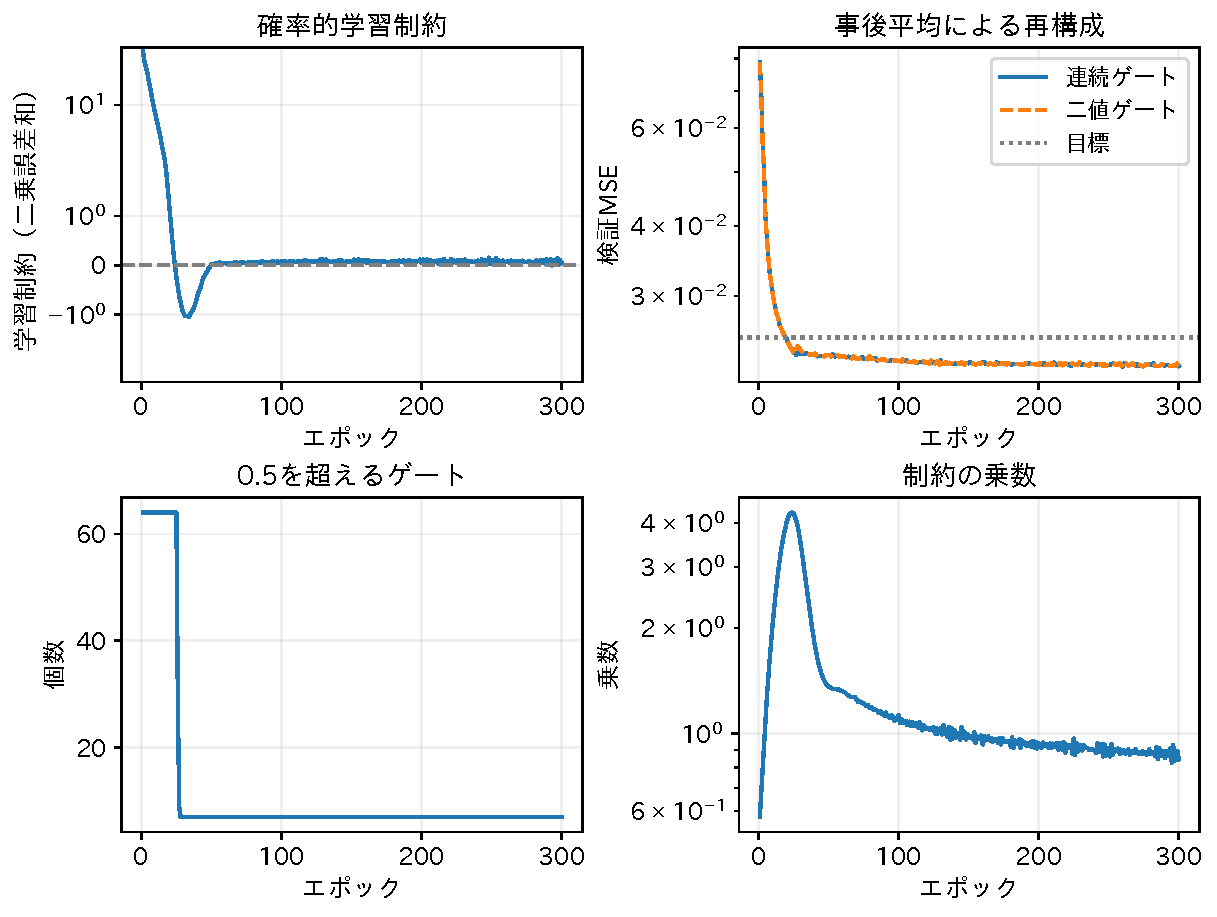
\includegraphics[width=\textwidth]{results/figures/NN53/native_hc.pdf}
\caption{新しいMNISTのhard-concrete実装診断。シード42，300 epochs。
学習制約は標本化した潜在変数とゲートを用い，検証は事後平均を用いる。
制約と再構成の推移に加え，ゲート数と乗数を示す。
独自HC実装の1実行であり，原著ARMの再現ではない。}
\label{fig:hc}
\end{figure}

ARD変更実装は，学習配列の先頭10\%（1800例）を事前分布の推定に確保し，残りで学習する。
10 epochsごとと学習終了後に$p_j=\operatorname{mean}(\mu_j^2+\sigma_j^2)$を更新し，
$[10^{-6},10^6]$に制限する。
これは固定部分集合で解析的な事後2次モーメントを使うものであり，
符号化データ集合を定期的に再標本化するものではない。
選択段階の学習は，再構成と重み1のガウスKLを用いる。
先頭512学習例について次式を計算する。
\begin{equation}
 w_j=\operatorname{mean}_{x,k}
 [g_k(\mu(x)+\sqrt{p_j}e_j)-g_k(\mu(x))]^2,
 \qquad q_j=w_jp_j,
 \label{eq:ardlocal}
\end{equation}
スコアを降順に並べ，合計の99\%に達する最小の個数を残す。
この有限差分は刻み幅の二乗で割っていない。
局所的には既に$p_j$の因子を含むため，さらに$p_j$を掛けると，
ヤコビアンの二乗と分散の積によるスコアとは異なる。
したがって保存個数は\emph{ARD変更実装}と呼び，文章の修正だけでこの相違は解消できない。
ガウス近似自体は原著からの逸脱ではない。
条件間で関連度配列と個数が同じであることを数値監査で確認した。
これは固定設定の反復であり，$\beta$の走査ではない。

保存された$q_j$と$p_j$があれば，checkpointなしでも有限刻み幅の余分な因子を除ける。
$h_j=\sqrt{p_j}$とすると，正しく正規化した有限刻み幅のスコアは次式となる。
\begin{equation}
 \widetilde q_j
 =p_j\,\operatorname{mean}_{x,k}
 \left[\frac{g_k(\mu+h_je_j)-g_k(\mu)}{h_j}\right]^2
 =\frac{q_j}{p_j}.
 \label{eq:ardcorrected}
\end{equation}
保存された$p_j$はすべて正である。
累積99\%の個数を再計算し，同じ最近傍グリッド規則で次元を転用する。
表\ref{tab:ard_normalized}では，CIFAR-10の未変換個数の平均は14.2から26.0へ変わり，
24次元へ写すと5試行すべてで$Q$を満たす。
これは保存数値の精度の範囲での，有限刻み幅の読み取りに対する代数的修正である。
刻み幅が大きい可能性と事前分布更新の変更は残るため，
厳密なヤコビアンや原著ARDのベンチマークではない。
\begin{table}[H]
\caption{主条件の保存スコアと事前分散から修正した，有限刻み幅の関連度読み取り。同じ保存摂動を刻み幅の二乗で正規化してから分散で重み付けし，新しいARD学習は行わない。検証するのは代数的な読み取り修正であり，厳密なヤコビアン関連度や原著学習手順ではない。test MSE（$10^3$倍）は次元転用先の通常VAEの値。}\label{tab:ard_normalized}
\small
\setlength{\tabcolsep}{3pt}
\begin{tabular*}{\textwidth}{@{\extracolsep{\fill}}lccccc@{}}
\toprule
データセット & 修正前個数 & 修正後個数 & 転用次元 & $Q$ & test MSE \\
\midrule
MNIST & $6.0 \pm 0.0$ & $6.2 \pm 0.4$ & $6.0 \pm 0.0$ & 5/5 & $22.05 \pm 0.17$ \\
Fashion-MNIST & $3.8 \pm 0.4$ & $4.0 \pm 0.0$ & $4.0 \pm 0.0$ & 5/5 & $19.06 \pm 0.25$ \\
dSprites & $9.2 \pm 1.5$ & $10.6 \pm 0.5$ & $10.0 \pm 0.0$ & 0/5 & $1.47 \pm 0.05$ \\
CIFAR-10 & $14.2 \pm 0.4$ & $26.0 \pm 0.0$ & $24.0 \pm 0.0$ & 5/5 & $15.36 \pm 0.13$ \\
\bottomrule\end{tabular*}
\end{table}

追加の厳密ヤコビアン実験は\ref{sec:newpruning}節で別に報告する。
これらは過去の記録を置き換えるものではない。

FONDUEの記述に基づく分類器は，公開リポジトリ
\url{https://github.com/bonheml/VAE_learning_dynamics}の
commit \texttt{f6d6e66b536bcbe635392d3438338949d4dc8730}と照合した。
独自実装は，1回の指数変換による事後分散の分類とTwoNNを用いる。
公開コードの実行経路や元の実験設定との同等性は主張しない。
過去の参照値として，原著は1 epochのdSprites選択を$12.2\pm0.4$と報告する\cite{bonheme2022fondue}が，
本研究の$\beta=1$では$4.2\pm0.4$である。
条件が揃っていないこの差は，実装誤りの証拠でも，元のベンチマークの再現でもない。
別の制御フロー検査では，保存されたID差系列に対し，原著アルゴリズムの上下限更新を再実行した。
FONDUEの全100経路と返却次元が疑似コードと一致し，通常終了した。
この検査は，それらの入力に対する探索更新ロジックを検証するものであり，
推定量の実装，学習フレームワークの同等性，公表ベンチマークを検証するものではない。
行ごとの結果を\path{results/make51/fondue_control_flow.json}に含める。

\subsection{閾値のみの解析と品質許容幅の解析}\label{app:sensitivity}
事後的予測解析はPython 3.11.11，NumPy 2.3.2，scikit-learn 1.7.1を用いる。
表\ref{tab:saturation}は，この再構成での確率飽和を示す。
元の予測器の完全な環境と行ごとの確率は保存されていないため，
集計値だけからその浮動小数点結果を厳密に確認できない。
今回の再構成の行ごとの決定スコアと確率は\path{results/make51/au_predictions.csv}に保存する。
\begin{table}[H]
\caption{今回の予測器再構成における確率の数値飽和。AUROC計算前にちょうど1へ丸められた予測の件数を示す。決定スコアではこれらの行の順位が保持される。}\label{tab:saturation}
\small
\setlength{\tabcolsep}{3.5pt}
\begin{tabular*}{\textwidth}{@{\extracolsep{\fill}}lccc@{}}
\toprule
評価条件 & 基準 & 基準+AU & 基準+無作為 \\
\midrule
dSprites & 55/55 & 44/55 & 49/55 \\
Fashion-MNIST & 0/55 & 0/55 & 0/55 \\
CIFAR-10 & 45/45 & 40/45 & 36/45 \\
\bottomrule
\end{tabular*}
\end{table}

本文のAU閾値図では，3つの$\delta$すべてに同じcheckpointを用いる。
重み列全体について，CIFAR-10のグリッド・シード候補のうち，AUが容量に等しい割合を以下に示す。
各$\beta$で10次元数と5シードを用いた件数であり，50個の独立したデータセットではない。
\begin{table}[H]
\caption{CIFAR-10（ガウス尤度）で，AUが容量に等しい候補の割合（\%）。分母は次元数・シードの50候補であり，各列では同じcheckpointから各閾値の個数を読み直す。}\label{tab:delta_rates}
\small
\setlength{\tabcolsep}{3.5pt}
\begin{tabular*}{\textwidth}{@{\extracolsep{\fill}}lccccc@{}}
\toprule
$\delta$ & $\beta=.25$ & $.5$ & $1$ & $2$ & $4$ \\
\midrule
0.001 & 100 & 100 & 100 & 98 & 60 \\
0.01 & 60 & 50 & 36 & 22 & 10 \\
0.1 & 48 & 38 & 32 & 20 & 10 \\
\bottomrule
\end{tabular*}
\end{table}

別の事後的な品質許容幅検査では，$\beta=1$の保存済み全グリッドを固定し，
再学習やアンカー変更をせず，各許容幅で目標を満たす最小次元を読み取る。
表\ref{tab:margin}はこの全グリッド基準を報告するもので，
制限された探索窓の選択器の経路や費用を報告するものではない。
FONDUEの閾値やARDの99\%基準に対する感度学習は実行していないため，
それら独自の読み取り閾値への応答は主張しない。
\begin{table}[H]
\caption{$\beta=1$で相対許容幅を変えた場合の，品質を満たす最小の保存次元数。5シードの平均$\pm$SD。検証分散の0.001倍という絶対下限は固定する。dSpritesはベルヌーイ，他はガウス尤度。}\label{tab:margin}
\footnotesize
\setlength{\tabcolsep}{3.5pt}
\begin{tabular*}{\textwidth}{@{\extracolsep{\fill}}lccccc@{}}
\toprule
データセット & 1\% & 5\% & 10\% & 25\% & 50\% \\
\midrule
MNIST & $6.0 \pm 0.0$ & $6.0 \pm 0.0$ & $6.0 \pm 0.0$ & $4.0 \pm 0.0$ & $4.0 \pm 0.0$ \\
Fashion-MNIST & $4.0 \pm 0.0$ & $4.0 \pm 0.0$ & $4.0 \pm 0.0$ & $4.0 \pm 0.0$ & $2.0 \pm 0.0$ \\
dSprites & $51.2 \pm 17.5$ & $36.0 \pm 16.5$ & $20.0 \pm 4.0$ & $12.0 \pm 0.0$ & $9.6 \pm 0.9$ \\
CIFAR-10 & $41.6 \pm 8.8$ & $32.0 \pm 0.0$ & $24.0 \pm 0.0$ & $16.0 \pm 0.0$ & $16.0 \pm 0.0$ \\
\bottomrule
\end{tabular*}
\end{table}

\section{合成データの尺度・除去診断}\label{app:synthetic}
Swiss rollの点は$(t\cos t,h,t\sin t)$で，
$t\sim U[1.5\pi,4.5\pi]$，$h\sim U[0,1]$とする。
トーラスの点は$((3+\cos\phi)\cos\theta,(3+\cos\phi)\sin\theta,\sin\phi)$で，
角度は独立に$[0,2\pi]$上の一様分布から得る。
各データは5000例，生成シード0とし，座標ごとに独立な標準偏差0.01のガウス雑音を加える。
先頭4500例を適合，残り500例を報告する診断に用いる。
保存実験では，各座標の標準化を分割前の全5000例に適合した。
これを前処理の情報漏洩として明示し，結果は記述的なものであり，情報漏洩のない独立test推定値とは扱わない。

全結合VAEは幅128，64と逆順の復号器，隠れ層のReLU，線形出力，
Adamの学習率$10^{-3}$，バッチ128，300 epochs，$\beta=1$，
シード42，123，777を用いる。
最後のcheckpointで，500診断例上の事後平均分散が0.01以下の座標をゼロにし，
同じ例上でMSEを再計算する。
表\ref{tab:synthetic}は標準化した実行を報告する。
この保存実験には別のtest集合はない。

\begin{table}[H]
\caption{合成データの尺度・除去診断。ガウス尤度，$\beta=1$，$\delta=0.01$，3学習シード。標準化は分割前に行ったため，記述的な検証結果であり，情報漏洩のない汎化推定ではない。変化は実行ごとのMSE相対変化の平均（\%）。}\label{tab:synthetic}
\footnotesize
\setlength{\tabcolsep}{3.5pt}
\begin{tabular*}{\textwidth}{@{\extracolsep{\fill}}lccccc@{}}
\toprule
データ & $m$ & AU & 除去前MSE & 除去後MSE & 変化 \\
\midrule
Swiss roll & 1 & $1.0 \pm 0.0$ & $0.3511 \pm 0.0267$ & $0.3511 \pm 0.0267$ & +0.000 \\
Swiss roll & 2 & $2.0 \pm 0.0$ & $0.1997 \pm 0.0177$ & $0.1997 \pm 0.0177$ & +0.000 \\
Swiss roll & 3 & $3.0 \pm 0.0$ & $0.1407 \pm 0.0018$ & $0.1407 \pm 0.0018$ & +0.000 \\
Swiss roll & 4 & $3.0 \pm 0.0$ & $0.1404 \pm 0.0136$ & $0.1406 \pm 0.0135$ & +0.147 \\
Swiss roll & 6 & $3.0 \pm 0.0$ & $0.1365 \pm 0.0023$ & $0.1368 \pm 0.0022$ & +0.183 \\
Swiss roll & 8 & $3.0 \pm 0.0$ & $0.1437 \pm 0.0089$ & $0.1440 \pm 0.0089$ & +0.165 \\
トーラス & 1 & $1.0 \pm 0.0$ & $0.3217 \pm 0.0163$ & $0.3217 \pm 0.0163$ & +0.000 \\
トーラス & 2 & $2.0 \pm 0.0$ & $0.1654 \pm 0.0242$ & $0.1654 \pm 0.0242$ & +0.000 \\
トーラス & 3 & $3.0 \pm 0.0$ & $0.1083 \pm 0.0036$ & $0.1083 \pm 0.0036$ & +0.000 \\
トーラス & 4 & $3.0 \pm 0.0$ & $0.1124 \pm 0.0050$ & $0.1124 \pm 0.0050$ & +0.063 \\
トーラス & 6 & $3.0 \pm 0.0$ & $0.1095 \pm 0.0035$ & $0.1096 \pm 0.0035$ & +0.107 \\
トーラス & 8 & $3.0 \pm 0.0$ & $0.1104 \pm 0.0069$ & $0.1105 \pm 0.0069$ & +0.156 \\
\bottomrule
\end{tabular*}
\end{table}

雑音のない両生成曲面の内在次元は2であり，ここでは3次元の外部座標で表現されている。
だからといって，Swiss rollのパッチの最小埋め込み次元が3になるわけではない。
この損失のもとで活性座標が3個観測されることは，位相の定理ではない。
以前の原稿は合成座標を標準化したと記載していたが，
実装監査ではその記述と実行された前処理の不一致が見つかった。
未標準化のSwiss rollでは高さ座標の分散が他の座標よりはるかに小さく，
二乗誤差上はその省略が安価になる。
この尺度の観測だけで，以前のAU結果すべての因果説明が完了するわけではない。

\section{新しいMNISTモデルの記録}\label{app:newmodels}
新実験は，候補となる12通りの次元数すべて，学習シード42，固定シードから再構成した元の分割を用いる。
モデル構造と目的関数は通常のMNIST手順に一致するが，CPU環境は過去のCUDA実行と異なる。
表\ref{tab:mcgrid}に，各proxy選択checkpointの検証基準をすべて示す。
MC SEは，事後標本化による評価雑音だけを表す。
容量選択を固定したファイルを，最終test評価に先立って保存する。
重み，epoch曲線，標本化ごとのELBO平均を査読用補足資料に含める。
この1シード検証から，学習シード間の信頼区間は推論しない。
\begin{table}[H]
\caption{新たに学習したMNISTの全グリッド。シード42，$\beta=1$，ガウス尤度。選択epochは決定論的proxyで選び，停止epochは実際の学習最終時点。proxyはガウス正規化定数と事後期待値を省くが，MC ELBOは両方を含む。MSEは$10^3$倍。}\label{tab:mcgrid}
\small
\setlength{\tabcolsep}{3pt}
\begin{tabular*}{\textwidth}{@{\extracolsep{\fill}}rrrrrc@{}}
\toprule
次元数 & 選択epoch & 停止epoch & 検証MSE & proxy & MC ELBO $\pm$ SE \\
\midrule
2 & 81 & 111 & 37.406 & $-34.647$ & $-484.386 \pm 0.009$ \\
4 & 85 & 115 & 27.840 & $-29.304$ & $-480.108 \pm 0.009$ \\
6 & 169 & 199 & 22.343 & $-26.696$ & $-478.174 \pm 0.010$ \\
8 & 73 & 103 & 22.417 & $-26.544$ & $-478.285 \pm 0.009$ \\
10 & 70 & 100 & 22.954 & $-26.663$ & $-478.627 \pm 0.009$ \\
12 & 196 & 226 & 20.983 & $-26.055$ & $-478.067 \pm 0.012$ \\
16 & 107 & 137 & 23.030 & $-26.774$ & $-478.592 \pm 0.009$ \\
20 & 144 & 174 & 21.327 & $-26.156$ & $-478.134 \pm 0.010$ \\
24 & 132 & 162 & 22.977 & $-26.956$ & $-478.664 \pm 0.008$ \\
32 & 136 & 166 & 23.402 & $-27.042$ & $-478.869 \pm 0.012$ \\
48 & 114 & 144 & 24.177 & $-27.411$ & $-479.310 \pm 0.013$ \\
64 & 217 & 247 & 22.930 & $-26.946$ & $-479.043 \pm 0.011$ \\
\bottomrule\end{tabular*}
\end{table}

\begin{figure}[!htbp]
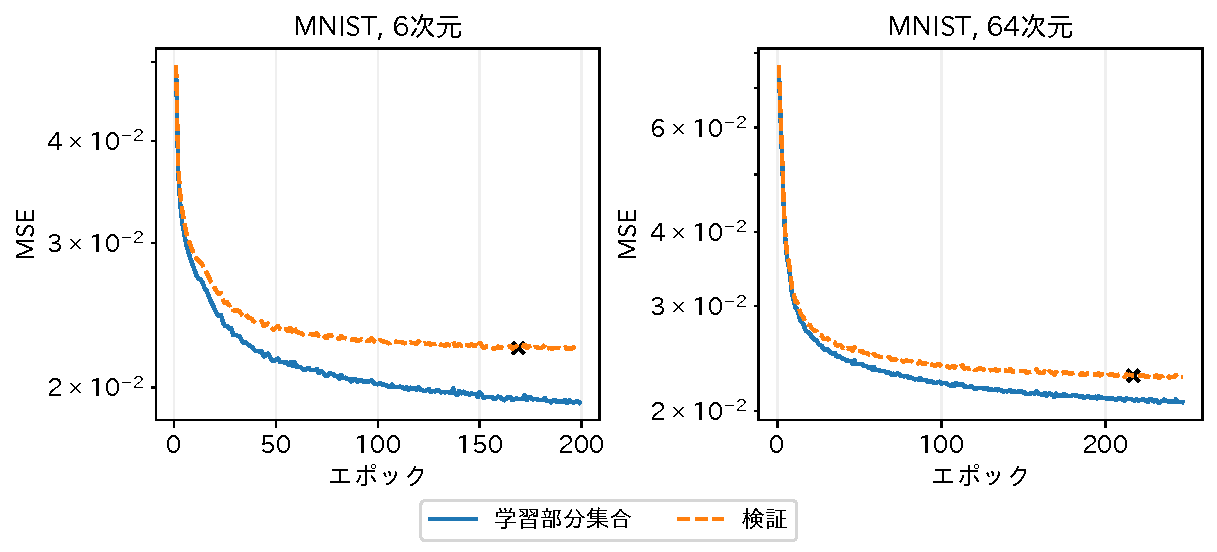
\includegraphics[width=\textwidth]{results/figures/NN53/new_mnist_curves.pdf}
\caption{新しいMNISTのシード42，6次元と64次元の学習・検証MSE。ガウス尤度，$\beta=1$。学習曲線は固定2000例の部分集合，検証は分離した全2000例を用いる。黒い十字はproxy選択epoch。新たに保存した実行であり，過去のCUDA checkpointの学習曲線を復元したものではない。}
\label{fig:newcurves}
\end{figure}

\section{追加GPU検証記録}\label{app:gpu}
表\ref{tab:newcounts}で過去と追加の読み取り値を比較する。
ARMのdSprites平均は54.0であり，過去のHC個数64とは異なる。
過去の未正規化CIFAR-10 ARD個数は14.2だったが，その正規化監査ですでに26.0へ修正されていた
（表\ref{tab:ard_normalized}）。
新しい厳密ヤコビアン個数は，この修正後の結果に近い。
学習と事前分布更新も変わっているため，14.2からの差全体をヤコビアン計算だけには帰属できない。
\begin{table}[H]
\caption{未変換の次元読み取り値。過去のHC・未正規化有限刻み幅ARD（5シード）と，新しいARM・厳密ヤコビアンARD（3シード）の比較。平均$\pm$標本SD。学習・読み取り設定が異なるため，すべての差を推定器だけに帰属できない。過去の有限刻み幅ARDの修正後結果は表\ref{tab:ard_normalized}に保持する。}\label{tab:newcounts}
\footnotesize
\setlength{\tabcolsep}{3pt}
\begin{tabular*}{\textwidth}{@{\extracolsep{\fill}}lccccc@{}}
\toprule
データセット & HC ($n=5$) & ARM ($n=3$) & 旧ARD（$n=5$） & 厳密・ゼロ & 厳密・標本 \\
\midrule
MNIST & $7.2 \pm 0.4$ & $7.7 \pm 0.6$ & $6.0 \pm 0.0$ & $6.0 \pm 0.0$ & $6.0 \pm 0.0$ \\
Fashion-MNIST & $4.2 \pm 0.4$ & $4.7 \pm 0.6$ & $3.8 \pm 0.4$ & $4.0 \pm 0.0$ & $4.0 \pm 0.0$ \\
dSprites & $64.0 \pm 0.0$ & $54.0 \pm 7.2$ & $9.2 \pm 1.5$ & $9.0 \pm 0.0$ & $9.7 \pm 0.6$ \\
CIFAR-10 & $20.0 \pm 1.0$ & $21.0 \pm 2.6$ & $14.2 \pm 0.4$ & $26.7 \pm 0.6$ & $26.3 \pm 0.6$ \\
\bottomrule\end{tabular*}
\end{table}

新しい記録は，ARMおよびARDの各分散更新設定について，各データセット3シードからなる。
表\ref{tab:armgates}のゲート区分と図\ref{fig:armconstraints}の個々の制約推移は，
閾値を超えた次元数だけでは剪定の成功を診断できない理由を示す。
特にdSpritesでは，明確な二値ゲート構成にも制約充足にも近づかない。
\begin{table}[H]
\caption{300 epochs後のARMゲート確率。中間は$0.1\le p\le0.9$，他の区分は厳密不等号を用いる。期待値は$\sum_j p_j$，個数は$p_j>0.5$で数える。dSpritesのゲートはどちらの極端な区分にも達しないため，閾値個数を安定した二値構造と解釈すべきではない。}\label{tab:armgates}
\small
\setlength{\tabcolsep}{3pt}
\begin{tabular*}{\textwidth}{@{\extracolsep{\fill}}lrrrrrr@{}}
\toprule
データセット & シード & $p<0.1$ & 中間 & $p>0.9$ & 期待値 & 個数 \\
\midrule
MNIST & 42 & 56 & 0 & 8 & 8.33 & 8 \\
MNIST & 123 & 56 & 1 & 7 & 8.11 & 8 \\
MNIST & 777 & 57 & 0 & 7 & 7.34 & 7 \\
Fashion-MNIST & 42 & 59 & 0 & 5 & 5.32 & 5 \\
Fashion-MNIST & 123 & 59 & 0 & 5 & 5.30 & 5 \\
Fashion-MNIST & 777 & 60 & 0 & 4 & 4.35 & 4 \\
dSprites & 42 & 0 & 64 & 0 & 32.08 & 52 \\
dSprites & 123 & 0 & 64 & 0 & 32.20 & 62 \\
dSprites & 777 & 0 & 64 & 0 & 32.05 & 48 \\
CIFAR-10 & 42 & 236 & 1 & 19 & 25.65 & 19 \\
CIFAR-10 & 123 & 230 & 3 & 23 & 30.27 & 24 \\
CIFAR-10 & 777 & 235 & 1 & 20 & 26.18 & 20 \\
\bottomrule\end{tabular*}
\end{table}

\begin{figure}[!htbp]
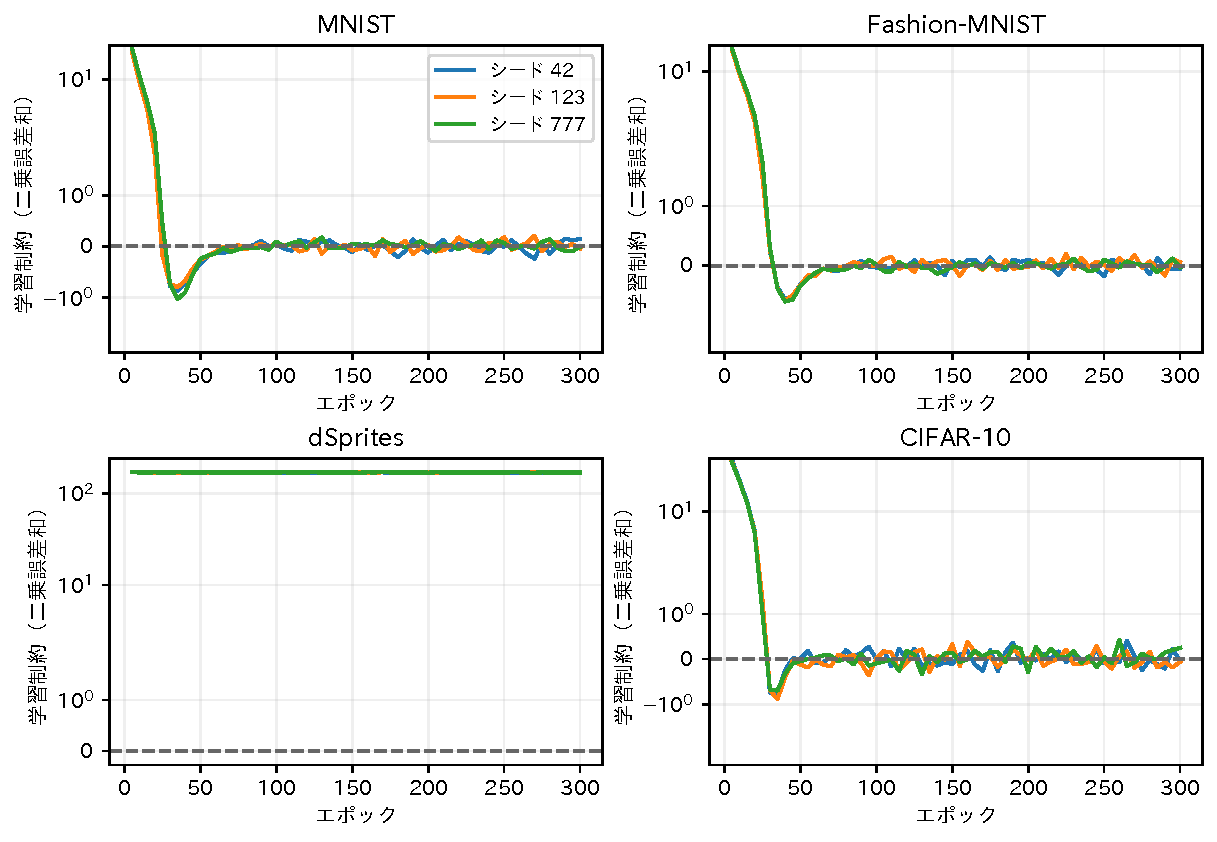
\includegraphics[width=\textwidth]{results/figures/NN53/arm_constraints.pdf}
\caption{新しいARM各シードの確率的学習制約の移動平均。5 epochsごとに記録した。ゼロが制約境界で，負値は制約充足を表す。大きな正の違反量と負値を表示するため，縦軸は対称対数尺度とする。これらの推移は，決定論的な検証目標の達成とは異なる。}
\label{fig:armconstraints}
\end{figure}

図\ref{fig:armcurves}および図\ref{fig:ardcurves}に，
全4データセットの評価モードでの再構成曲線を示す。
これらは提供された300 epochsの実行を記述するものであり，
曲線が視覚的に平坦でも最適性を保証しない。
ARDの図はゼロ中心の分散更新を用いる。
標本平均を中心とする変種を含む全24件のARD曲線記録は補足資料に収録する。

\begin{figure}[!htbp]
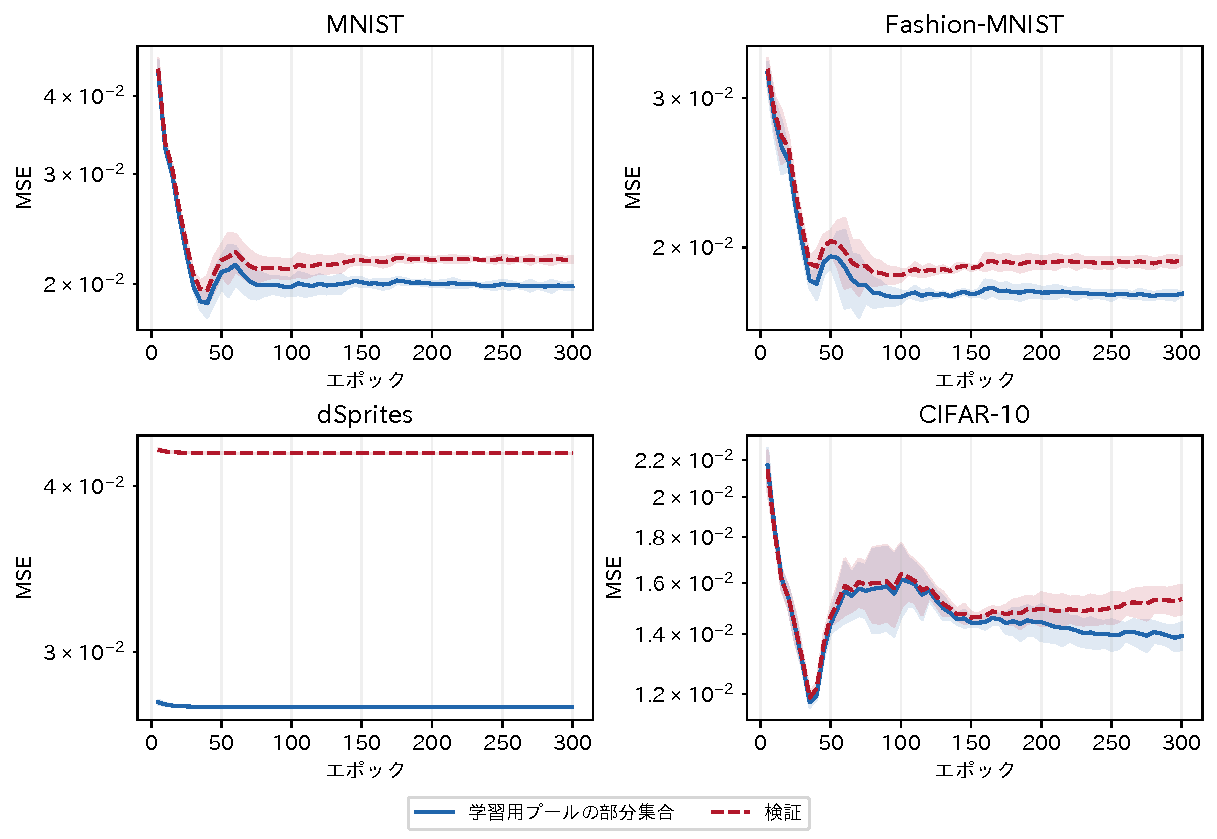
\includegraphics[width=\textwidth]{results/figures/NN53/arm_curves.pdf}
\caption{その時点の二値ゲートマスクを用いたnative ARMの事後平均MSE。学習2000例の部分集合と検証分割で5 epochsごとに評価した。線と陰影は3シードの平均と標本SD。縦軸は対数尺度で，表示のため陰影の下限を正値に制限する。欠けている過去の通常VAE学習記録を再構成した曲線ではない。}
\label{fig:armcurves}
\end{figure}

\begin{figure}[!htbp]
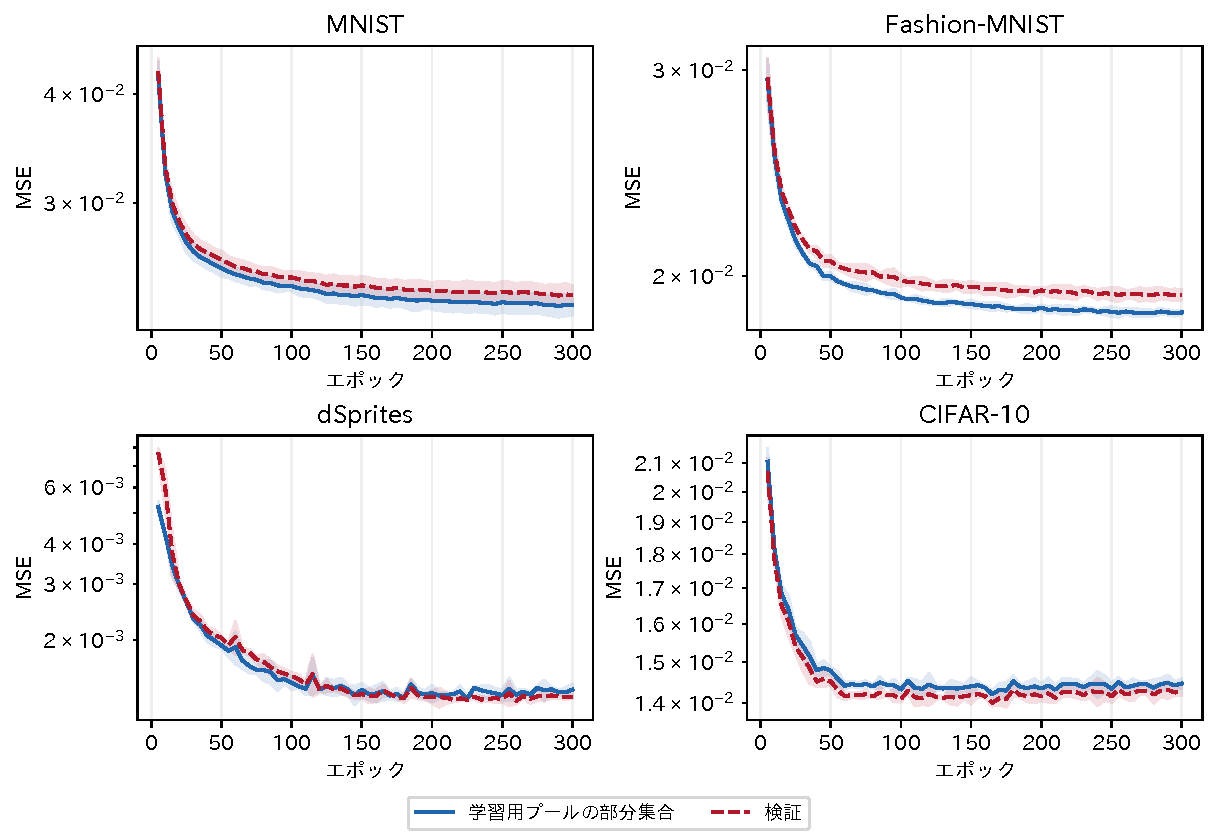
\includegraphics[width=\textwidth]{results/figures/NN53/ard_curves.pdf}
\caption{ゼロ中心の分散更新を用いた，全次元ARDの事後平均MSE。5 epochsごとに評価し，3シードの平均と標本SDを示す。縦軸は対数尺度。学習用プールの2000例の部分集合には，事前分布更新専用の1800例とパラメータ勾配学習に用いた200例が含まれるため，純粋な学習適合度の推定ではない。これらの評価ではnativeモデルを剪定していない。}
\label{fig:ardcurves}
\end{figure}

表\ref{tab:newtest}に，固定した最終nativeモデルと転用先の通常次元における，
分離したtest再構成を示す。
選択には制約または検証データに基づく関連度読み取りを用い，これらのtest指標は用いない。
ARDの全次元モデル列を，選択されたnative次元での品質と明確に区別する。
\begin{table}[H]
\caption{test MSE（$10^3$倍）。3シードの平均$\pm$標本SD。ARMのnative評価は二値ゲートマスクと事後平均を用いる。ARDのnative評価は未剪定の全次元モデルを用いる。転用先通常VAEは過去の候補キャッシュから再利用したもので，そのtest集計は新しい未変換個数の選択に用いていない。}\label{tab:newtest}
\small
\setlength{\tabcolsep}{3pt}
\begin{tabular*}{\textwidth}{@{\extracolsep{\fill}}llcc@{}}
\toprule
データセット & 実装 & native／全次元 & 転用 \\
\midrule
MNIST & ARM & $21.35 \pm 0.25$ & $21.22 \pm 0.79$ \\
MNIST & ARD・ゼロ & $22.97 \pm 0.53$ & $22.15 \pm 0.14$ \\
MNIST & ARD・標本 & $23.17 \pm 0.17$ & $22.15 \pm 0.14$ \\
Fashion-MNIST & ARM & $19.01 \pm 0.23$ & $18.94 \pm 0.23$ \\
Fashion-MNIST & ARD・ゼロ & $18.97 \pm 0.17$ & $18.94 \pm 0.23$ \\
Fashion-MNIST & ARD・標本 & $19.17 \pm 0.15$ & $18.94 \pm 0.23$ \\
dSprites & ARM & $42.10 \pm 0.00$ & $1.17 \pm 0.04$ \\
dSprites & ARD・ゼロ & $1.32 \pm 0.01$ & $1.86 \pm 0.09$ \\
dSprites & ARD・標本 & $1.32 \pm 0.06$ & $1.61 \pm 0.30$ \\
CIFAR-10 & ARM & $15.60 \pm 0.59$ & $16.74 \pm 1.21$ \\
CIFAR-10 & ARD・ゼロ & $14.55 \pm 0.13$ & $15.42 \pm 0.13$ \\
CIFAR-10 & ARD・標本 & $14.64 \pm 0.24$ & $15.42 \pm 0.13$ \\
\bottomrule\end{tabular*}
\end{table}

表\ref{tab:newcost}は，記録された所要時間の構成要素を示す。
出所記録にはNVIDIA GPUとソフトウェア環境が記載されている。
学習区間には定期評価を含む。
ARDの初回・最終の事前分布更新と最終native評価は，
表示した学習・ヤコビアン時間の区間には含まれない。
ヤコビアン時間は検証100例と当該ネットワーク構造に対するものである。
参照群，アンカー，転用，評価の費用に欠落があるため，
これらを選択器の全費用と解釈したり，過去のCPUによるID時間と合算したりすることはできない。
\begin{table}[H]
\caption{新しいGPU剪定実験の記録時間内訳。単位は秒，3シードの平均$\pm$標本SD。学習ループには定期的な学習・検証評価を含む。ARMの事後評価は最終native評価を含むが，ARDではその時間を個別に記録していない（未記録）。アンカー，転用候補，その他の欠落費用は含まない。これらは完全なend-to-end選択器費用ではない。}\label{tab:newcost}
\small
\setlength{\tabcolsep}{3pt}
\begin{tabular*}{\textwidth}{@{\extracolsep{\fill}}llccc@{}}
\toprule
データセット & 実装 & 学習ループ & ヤコビアン & 事後評価 \\
\midrule
MNIST & ARM & $197.8 \pm 2.2$ & --- & $0.043 \pm 0.000$ \\
MNIST & ARD・ゼロ & $87.3 \pm 0.3$ & $0.011 \pm 0.000$ & 未記録 \\
MNIST & ARD・標本 & $87.1 \pm 0.7$ & $0.012 \pm 0.002$ & 未記録 \\
Fashion-MNIST & ARM & $197.8 \pm 1.5$ & --- & $0.043 \pm 0.000$ \\
Fashion-MNIST & ARD・ゼロ & $88.2 \pm 0.5$ & $0.011 \pm 0.000$ & 未記録 \\
Fashion-MNIST & ARD・標本 & $88.0 \pm 0.3$ & $0.012 \pm 0.002$ & 未記録 \\
dSprites & ARM & $664.8 \pm 0.3$ & --- & $1.264 \pm 0.001$ \\
dSprites & ARD・ゼロ & $299.2 \pm 0.0$ & $10.830 \pm 0.169$ & 未記録 \\
dSprites & ARD・標本 & $299.2 \pm 0.2$ & $11.047 \pm 0.712$ & 未記録 \\
CIFAR-10 & ARM & $328.4 \pm 0.3$ & --- & $0.570 \pm 0.001$ \\
CIFAR-10 & ARD・ゼロ & $146.2 \pm 0.1$ & $6.968 \pm 0.452$ & 未記録 \\
CIFAR-10 & ARD・標本 & $146.1 \pm 0.1$ & $7.505 \pm 0.171$ & 未記録 \\
\bottomrule\end{tabular*}
\end{table}

\subsection{Nativeマスクと復号器微調整}
表\ref{tab:ardprunedseeds}と表\ref{tab:ardprunedtest}に，
native剪定の4条件についてシード別の検証記録と保持されたtest集合の集計を示す。
選択個数は先行する標本中心の実行と一致する。
未剪定の検証・test MSEも一致するため，繰り返された基準値は追加の独立した根拠ではない。
dSpritesのtest平均は検証と同じ傾向を示し，
マスク前0.00132，マスク後0.00294，復号器微調整後0.00178となる。
\begin{table}[H]
\caption{シードごとのnative剪定の検証MSE（$10^3$倍）。個数は関連度で選択した軸数，グリッドは転用先通常VAEの次元数。全次元，マスク，微調整は事後平均を用いる。標本マスクは微調整前の32事後標本による平均MSEであり，ELBOでも標本アンカー目標による比較でもない。マスクそのものとモデルcheckpointは保存されていない。}\label{tab:ardprunedseeds}
\footnotesize
\setlength{\tabcolsep}{3pt}
\begin{tabular*}{\textwidth}{@{\extracolsep{\fill}}lrrrrrrr@{}}
\toprule
データセット & シード & 個数 & グリッド & 全次元 & マスク & 微調整 & 標本マスク \\
\midrule
MNIST & 42 & 6 & 6 & $23.762$ & $23.772$ & $23.445$ & $27.040$ \\
MNIST & 123 & 6 & 6 & $23.669$ & $23.681$ & $23.454$ & $27.050$ \\
MNIST & 777 & 6 & 6 & $23.410$ & $23.420$ & $23.175$ & $26.896$ \\
Fashion-MNIST & 42 & 4 & 4 & $19.336$ & $19.340$ & $19.158$ & $21.573$ \\
Fashion-MNIST & 123 & 4 & 4 & $19.452$ & $19.456$ & $19.248$ & $21.732$ \\
Fashion-MNIST & 777 & 4 & 4 & $19.496$ & $19.496$ & $19.176$ & $21.563$ \\
dSprites & 42 & 10 & 10 & $1.393$ & $3.317$ & $1.893$ & $3.611$ \\
dSprites & 123 & 10 & 10 & $1.278$ & $2.783$ & $1.727$ & $3.084$ \\
dSprites & 777 & 9 & 8 & $1.327$ & $2.945$ & $1.859$ & $3.223$ \\
CIFAR-10 & 42 & 26 & 24 & $14.668$ & $15.109$ & $14.817$ & $17.584$ \\
CIFAR-10 & 123 & 26 & 24 & $14.192$ & $14.728$ & $14.671$ & $17.253$ \\
CIFAR-10 & 777 & 27 & 24 & $14.353$ & $14.835$ & $14.692$ & $17.392$ \\
\bottomrule\end{tabular*}
\end{table}

\begin{table}[H]
\caption{Native剪定のtest MSE（$10^3$倍）。3シードの平均$\pm$標本SD。全列で事後平均による再構成を用いる。条件は表\ref{tab:ardpruned}と同じであり，test指標は軸や固定微調整予算の選択に用いない。}\label{tab:ardprunedtest}
\small
\setlength{\tabcolsep}{3pt}
\begin{tabular*}{\textwidth}{@{\extracolsep{\fill}}lcccc@{}}
\toprule
データセット & 全次元 & マスク & 微調整 & Transfer \\
\midrule
MNIST & $23.17 \pm 0.17$ & $23.18 \pm 0.17$ & $22.90 \pm 0.14$ & $22.15 \pm 0.14$ \\
Fashion-MNIST & $19.17 \pm 0.15$ & $19.17 \pm 0.15$ & $18.93 \pm 0.08$ & $18.94 \pm 0.23$ \\
dSprites & $1.32 \pm 0.06$ & $2.94 \pm 0.25$ & $1.78 \pm 0.07$ & $1.61 \pm 0.30$ \\
CIFAR-10 & $14.64 \pm 0.24$ & $15.14 \pm 0.19$ & $14.97 \pm 0.08$ & $15.42 \pm 0.13$ \\
\bottomrule\end{tabular*}
\end{table}

表\ref{tab:ardprunedcost}は，記録された2種類の時間区間を示す。
先行する曲線取得実験とは異なり，初期学習の時間区間は定期評価を含まず，最後の事前分布更新を含む。
最初の事前分布更新，ヤコビアン評価，マスク生成，最終モデル評価は，記録された時間区間の外である。
したがって，学習時間と微調整時間を足しても，剪定のend-to-end費用にはならない。
提供されたスクリプトは300 epochsの学習と30 epochsの微調整プロトコルを定義するが，
JSONにはepochカウンタや推移がない。
これらの設定はスクリプトと内部仕様から記述したもので，保存された学習履歴から独立に復元したものではない。
\begin{table}[H]
\caption{Native剪定実行の部分的な時間計測。単位は秒，3シードの平均$\pm$標本SD。学習時間は最後の事前分布更新を含むが，最初の更新を含まない。微調整時間は復号器の30 epochsのループのみを計測する。ヤコビアン・マスクの生成，最終評価，アンカーおよび転用先の学習は含まず，この実行では個別に計測していない。}\label{tab:ardprunedcost}
\small
\setlength{\tabcolsep}{3pt}
\begin{tabular*}{\textwidth}{@{\extracolsep{\fill}}lcc@{}}
\toprule
データセット & 学習区間 & 復号器微調整 \\
\midrule
MNIST & $86.5 \pm 0.7$ & $5.9 \pm 0.1$ \\
Fashion-MNIST & $86.5 \pm 0.4$ & $5.9 \pm 0.0$ \\
dSprites & $289.0 \pm 0.3$ & $20.7 \pm 0.0$ \\
CIFAR-10 & $142.3 \pm 0.1$ & $10.8 \pm 0.0$ \\
\bottomrule\end{tabular*}
\end{table}

記録された\texttt{elbo}と\texttt{val\_elbo}欄は，来歴のため未変更のrawファイルに保持するが，
新しいマスク記録も含め，native ELBOの測定値として用いない（\ref{sec:gpuvalidation}節）。
マスク後のnative MSEは今回記録されたが，checkpointと選択軸の識別子は保存されていない。
したがって，集計だけからマスク，推論出力，修正されたnative尤度を独立に再評価することはできない。
解析的なARM勾配検査は成分を検証するもので，これらのモデル単位の記録を代替しない。

\section{再現性のためのファイル一覧と残る記録}\label{app:inventory}
再集計の入口は\path{src/make51/rebuild_review.py}である。
保存済みJSONと設定ファイルを読み，過去の記録から数値表，6図，対応のある予測解析を出力する。
新しい探索解析は\path{src/make51/replay_search.py}，
限定的なモデル検証は\path{src/make51/validate_models.py}である。
その出力は\path{src/make51/summarize_validation.py}で集計する。
追加実行の再集計は\path{src/make52/summarize_revision.py}，
native剪定の再集計は\path{src/make53/summarize_native_pruning.py}，
原稿の組立ては\path{src/make53/build_manuscript.py}である。
生成された主TeXは表の内容を埋め込み，図PDFを参照する。
英語版はプロジェクト直下で\texttt{pdflatex}を参照が確定するまで繰り返してコンパイルする。
同梱の\texttt{MAKE53\_reproducibility.zip}は，この一覧だけでなくファイル自体を提供する。
READMEは軽量な再集計と任意の再学習を区別し，依存環境の版と利用できない過去の成果物を示す。
\texttt{MANIFEST.sha256}が収録内容を識別する。
アーカイブは固定されたソースのsnapshotを含み，非公開リポジトリへのアクセスなしで利用できる。

\begin{table}[H]
\caption{本改訂のソースと出力の対応。ディレクトリはプロジェクト直下からの相対表記。補足資料のREADMEに個別ファイル名と再集計コマンドを示す。}
\label{tab:inventory}\footnotesize
\begin{tabularx}{\textwidth}{lX}\toprule
証拠 & ファイル・ディレクトリ \\\midrule
設定 & \path{config/} \\
過去の手法・推移・診断記録 & \path{results/make49/} \\
候補指標と潜在分散 & \path{results/make49/stage4_cache/} \\
探索・AU・過去の監査の集計 & \path{results/make51/} \\
別途のMNISTモデル・MC ELBO記録 & \path{results/make51/model_validation/} \\
判定付き開始点・ARM・ARD・nativeマスクのraw記録 & \path{results/make52/} \\
Nativeマスク集計・ソースハッシュ & \path{results/make53/} \\
過去と追加の学習コード & \path{src/make49/}; \path{src/make52/} \\
過去と追加の再集計 & \path{src/make51/}; \path{src/make53/} \\
英語原稿テンプレート & \path{src/make53/} \\
日本語訳と検証 & \path{src/nn53/}; \path{results/nn53/} \\
英語図 & \path{results/figures/MAKE51/}; \path{results/figures/MAKE52/} \\
日本語図 & \path{results/figures/NN53/} \\
\bottomrule\end{tabularx}
\end{table}

手法単位の行の識別子は，データセット，手法，候補シード，$\beta$または条件である。
候補キーには次元数，指定epoch数，停止設定も含まれる。
主たる手法記録の各設定・データセット・手法・条件の組合せに5シードがあることを，再集計中に確認する。
ARDの反復によって，異なる選択重み条件が5個生じるわけではない。
初期のグリッド外キャッシュ項目はすべて残っているわけではないが，
最終指標と学習traceは手法記録に残る。
元のtest予測，過去の完全なモデルcheckpoint，独立したID・評価時間は，欠けたファイルから復元しない。

内部の変更記録には，9月12日の初期仕様，崩壊診断後のdSpritesのベルヌーイ尤度への変更，
実現不能な検証10,000例の抽出から学習データの利用へのID推定標本の変更，
早期停止なしの推移実行，9月13日の参照次元・実行費用計上・退化出力の明確化が記録されている。
主要な予測解析の後には無作為特徴量対照を追加した。
本改訂のアンカー費用補完，対応付きAU推論，品質許容幅の読み直し，明示的実装監査は事後的である。
いずれも公開の事前登録済み検定とは言い換えない。
9月19日の局所方策，閾値の全組合せ，正規化したARD読み取り，新たな1シード検証は，先の結果の後に仕様を定めた。
補足資料には，それぞれの仕様と出力場所を保持する。

追加の開始次元数・剪定記録は，別途の事後解析である。
再集計では，統合ファイルとデータセット別ファイルの一致，3シードの網羅性，
300 epochsの曲線終点，未変換個数の読み取り，アンカー目標，転用先キャッシュ指標を検査する。
これは提供記録の整合性を検証するもので，利用できないcheckpointの再実行一致を検証するものではない。
新しいnativeマスク監査ではさらに，12件すべてをデータセット別ファイル，
先行する標本中心の全次元モデルのMSE・個数，転用候補キャッシュと照合し，
$Q$と対応のある集計を再計算する。
未保存のマスクやcheckpointテンソルは復元できない。

\paragraph{日本語版の生成}
日本語本文の組立ては\path{src/nn53/build_japanese.py}，
図の表示文字の日本語化は\path{src/nn53/render_figures.py}による。
日本語TeXのコンパイルには，プロジェクト直下で
\texttt{lualatex main\_paper\_NN53.tex}を参照が確定するまで繰り返す。
日本語図は\path{results/figures/NN53/}に保存する。


\begin{thebibliography}{999}

\bibitem{kingma2014vae}
Kingma, D.P.; Welling, M.
Auto-encoding variational Bayes.
In \textit{Proceedings of the 2nd International Conference on Learning
Representations (ICLR)}, Banff, AB, Canada, 14--16 April 2014.
arXiv:1312.6114. \url{https://doi.org/10.48550/arXiv.1312.6114}.

\bibitem{facco2017twonn}
Facco, E.; d'Errico, M.; Rodriguez, A.; Laio, A.
Estimating the intrinsic dimension of datasets by a minimal neighborhood
information.
\textit{Sci.\ Rep.} \textbf{2017}, \textit{7}, 12140.
\url{https://doi.org/10.1038/s41598-017-11873-y}.

\bibitem{levina2005mle}
Levina, E.; Bickel, P.J.
Maximum likelihood estimation of intrinsic dimension.
In \textit{Advances in Neural Information Processing Systems},
\textbf{2004}, \textit{17}.
\url{https://proceedings.neurips.cc/paper/2004/hash/74934548253bcab8490ebd74afed7031-Abstract.html}.

\bibitem{bonheme2022fondue}
Bonheme, L.; Grzes, M.
FONDUE: An algorithm to find the optimal dimensionality of the latent
representations of variational autoencoders.
arXiv \textbf{2022}, arXiv:2209.12806.
\url{https://doi.org/10.48550/arXiv.2209.12806}.

\bibitem{burda2016iwae}
Burda, Y.; Grosse, R.; Salakhutdinov, R.
Importance weighted autoencoders.
In \textit{Proceedings of the 4th International Conference on Learning
Representations (ICLR)}, San Juan, Puerto Rico, 2--4 May 2016.
arXiv:1509.00519. \url{https://doi.org/10.48550/arXiv.1509.00519}.

\bibitem{bonheme2023active}
Bonheme, L.; Grzes, M.
Be more active! Understanding the differences between mean and sampled
representations of variational autoencoders.
\textit{J. Mach. Learn. Res.} \textbf{2023}, \textit{24}(324), 1--30.
\url{https://jmlr.org/papers/v24/21-1145.html}.

\bibitem{deboom2020geco}
De Boom, C.; Wauthier, S.; Verbelen, T.; Dhoedt, B.
Dynamic narrowing of VAE bottlenecks using GECO and $L_0$ regularization.
arXiv \textbf{2020}, arXiv:2003.10901.
\url{https://doi.org/10.48550/arXiv.2003.10901}.

\bibitem{saha2025ardvae}
Saha, S.; Joshi, S.; Whitaker, R.
ARD-VAE: A statistical formulation to find the relevant latent dimensions
of variational autoencoders.
arXiv \textbf{2025}, arXiv:2501.10901.
\url{https://doi.org/10.48550/arXiv.2501.10901}.

\bibitem{tippingbishop1999ppca}
Tipping, M.E.; Bishop, C.M.
Probabilistic principal component analysis.
\textit{J.\ R.\ Stat.\ Soc.\ Ser.\ B} \textbf{1999}, \textit{61}, 611--622.
\url{https://doi.org/10.1111/1467-9868.00196}.

\bibitem{tenenbaum2000isomap}
Tenenbaum, J.B.; de Silva, V.; Langford, J.C.
A global geometric framework for nonlinear dimensionality reduction.
\textit{Science} \textbf{2000}, \textit{290}, 2319--2323.
\url{https://doi.org/10.1126/science.290.5500.2319}.

\bibitem{roweis2000lle}
Roweis, S.T.; Saul, L.K.
Nonlinear dimensionality reduction by locally linear embedding.
\textit{Science} \textbf{2000}, \textit{290}, 2323--2326.
\url{https://doi.org/10.1126/science.290.5500.2323}.

\bibitem{ceruti2014danco}
Ceruti, C.; Bassis, S.; Rozza, A.; Lombardi, G.; Casiraghi, E.;
Campadelli, P.
DANCo: An intrinsic dimensionality estimator exploiting angle and norm
concentration.
\textit{Pattern Recognit.} \textbf{2014}, \textit{47}, 2569--2581.
\url{https://doi.org/10.1016/j.patcog.2014.02.013}.

\bibitem{johnsson2015ess}
Johnsson, K.; Soneson, C.; Fontes, M.
Low bias local intrinsic dimension estimation from expected simplex
skewness.
\textit{IEEE Trans.\ Pattern Anal.\ Mach.\ Intell.} \textbf{2015},
\textit{37}, 196--202. \url{https://doi.org/10.1109/TPAMI.2014.2343220}.

\bibitem{costa2004geodesic}
Costa, J.A.; Hero, A.O.
Geodesic entropic graphs for dimension and entropy estimation in manifold
learning.
\textit{IEEE Trans.\ Signal Process.} \textbf{2004}, \textit{52},
2210--2221. \url{https://doi.org/10.1109/TSP.2004.831130}.

\bibitem{camastra2016intrinsic}
Camastra, F.; Staiano, A.
Intrinsic dimension estimation: Advances and open problems.
\textit{Inf.\ Sci.} \textbf{2016}, \textit{328}, 26--41.
\url{https://doi.org/10.1016/j.ins.2015.08.029}.

\bibitem{allegra2020data}
Allegra, M.; Facco, E.; Denti, F.; Laio, A.; Mira, A.
Data segmentation based on the local intrinsic dimension.
\textit{Sci.\ Rep.} \textbf{2020}, \textit{10}, 16449.
\url{https://doi.org/10.1038/s41598-020-72222-0}.

\bibitem{galka2022isolation}
Ga{\l}ka, {\L}.; Karczmarek, P.; Tokovarov, M.
Isolation Forest Based on Minimal Spanning Tree.
\textit{IEEE Access} \textbf{2022}, \textit{10}, 74175--74186.
\url{https://doi.org/10.1109/ACCESS.2022.3190505}.

\bibitem{ansuini2019intrinsic}
Ansuini, A.; Laio, A.; Macke, J.H.; Zoccolan, D.
Intrinsic dimension of data representations in deep neural networks.
In \textit{NeurIPS 2019}, Vol.~32, 2019. \url{https://proceedings.neurips.cc/paper_files/paper/2019/file/cfcce0621b49c983991ead4c3d4d3b6b-Paper.pdf}.

\bibitem{pope2021intrinsic}
Pope, P.; Zhu, C.; Abdelkader, A.; Goldblum, M.; Goldstein, T.
The intrinsic dimension of images and its impact on learning.
In \textit{ICLR 2021}, 2021. arXiv:2104.08894. \url{https://doi.org/10.48550/arXiv.2104.08894}.

\bibitem{rezende2018geco}
Rezende, D.J.; Viola, F.
Taming VAEs.
arXiv \textbf{2018}, arXiv:1810.00597.
\url{https://doi.org/10.48550/arXiv.1810.00597}.

\bibitem{louizos2018l0}
Louizos, C.; Welling, M.; Kingma, D.P.
Learning sparse neural networks through $L_0$ regularization.
In \textit{Proceedings of the 6th International Conference on Learning
Representations (ICLR)}, Vancouver, BC, Canada, 30 April--3 May 2018.
arXiv:1712.01312. \url{https://doi.org/10.48550/arXiv.1712.01312}.

\bibitem{obata2025manifold}
Obata, C.; Jin'no, K.
Analysis of the relationship between manifold structure and latent space
capacity of input data using VAE.
In \textit{Proceedings of the 2025 International Symposium on Nonlinear
Theory and Its Applications (NOLTA2025)}, Okinawa, Japan, 27--31 October
2025; pp. 32--35.
Publication record: \url{https://www.comm.tcu.ac.jp/nel/list_j_2025.html}
(accessed on 18 September 2026).

\bibitem{whitney1944}
Whitney, H.
The self-intersections of a smooth $n$-manifold in $2n$-space.
\textit{Ann. Math.} \textbf{1944}, \textit{45}, 220--246.
\url{https://doi.org/10.2307/1969265}.

\bibitem{lucas2019elbo}
Lucas, J.; Tucker, G.; Grosse, R.B.; Norouzi, M.
Don't blame the ELBO! A linear VAE perspective on posterior collapse.
In \textit{NeurIPS 2019}, Vol.~32, 2019. \url{https://proceedings.neurips.cc/paper/2019/file/7e3315fe390974fcf25e44a9445bd821-Paper.pdf}.

\bibitem{rolinek2019pca}
Rolinek, M.; Zietlow, D.; Martius, G.
Variational autoencoders pursue PCA directions (by accident).
In \textit{Proceedings of the IEEE/CVF Conference on Computer Vision and
Pattern Recognition (CVPR)}, Long Beach, CA, USA, 15--20 June 2019;
pp.\ 12406--12415. \url{https://doi.org/10.1109/CVPR.2019.01269}.

\bibitem{lecun1998}
LeCun, Y.; Bottou, L.; Bengio, Y.; Haffner, P.
Gradient-based learning applied to document recognition.
\textit{Proc.\ IEEE} \textbf{1998}, \textit{86}, 2278--2324.
\url{https://doi.org/10.1109/5.726791}.

\bibitem{xiao2017fashion}
Xiao, H.; Rasul, K.; Vollgraf, R.
Fashion-{MNIST}: A Novel Image Dataset for Benchmarking Machine Learning
Algorithms.
\textit{arXiv} \textbf{2017}, 1708.07747. \url{https://doi.org/10.48550/arXiv.1708.07747}.

\bibitem{krizhevsky2009learning}
Krizhevsky, A.
Learning multiple layers of features from tiny images.
\textit{Technical Report}; University of Toronto: Toronto, ON, Canada,
2009.

\bibitem{matthey2017dsprites}
Matthey, L.; Higgins, I.; Hassabis, D.; Lerchner, A.
dSprites: Disentanglement testing sprites dataset. 2017.
Available online: \url{https://github.com/google-deepmind/dsprites-dataset}
(accessed on 12 September 2026).

\bibitem{fu2019cyclical}
Fu, H.; Li, C.; Liu, X.; Gao, J.; Celikyilmaz, A.; Carin, L.
Cyclical annealing schedule: A simple approach to mitigating KL vanishing.
In \textit{Proceedings of NAACL-HLT 2019}, Minneapolis, MN, USA, 2019;
pp.~240--250. \url{https://doi.org/10.18653/v1/N19-1021}.

\end{thebibliography}
\end{document}
